\documentclass[conference]{IEEEtran}

\usepackage{cite}
\usepackage{amsmath,amssymb,amsfonts}
\usepackage{algorithmic}
\usepackage{graphicx}
\usepackage{textcomp}
\usepackage{xcolor}
\usepackage{gensymb}
\usepackage{tikz}
\usepackage{float}
\usepackage{hyperref}
\usepackage{enumerate}
\usepackage{subcaption}
\def\BibTeX{{\rm B\kern-.05em{\sc i\kern-.025em b}\kern-.08em
    T\kern-.1667em\lower.7ex\hbox{E}\kern-.125emX}}
\begin{document}

\title{4-Bit CLA Adder \\ VLSI Course Project}

\author{\IEEEauthorblockN{1\textsuperscript{st} Vignesh Vembar}
\IEEEauthorblockA{\textit{ECE, IIIT Hyderabad} \\
\textit{2023102019}\\
vigneshvembar.m@students.iiit.ac.in}
}

\maketitle

\begin{abstract}
This document is a report on the Design and Simulation of a 4-bit Carry Look Ahead Adder.
\end{abstract}


\section{Introduction}
The Carry Look Ahead Adder is a digital circuit that is used to add two 4 bit binary numbers. It is faster than the Ripple Carry Adder as it generates the carry signals for all the bits at the same time. We will also be passing the inputs and outputs through D Flip Flops to make the circuit synchronous.

\section{Proposed Design}

\subsection{CLA Adder} 
\cite{b1} From the given inputs signals, we first generate Propagate and Generate signals. These are defined as follows \footnote{An optimization here could be to use the + operator to calculate Propagate instead of $\oplus$. Unfortunately, I did not have this insight until too late in the project.}:

\begin{align}
    P_i &= A_i \oplus B_i \\
    G_i &= A_i \cdot B_i
\end{align}

Then, the carry signals can be generated as follows:

\begin{align}
    C_{i+1} &= G_i + P_i \cdot C_i
\end{align}

In reality, we use multi-input gates to calculate these carries instead of recursively. This is done using the following equations:

\begin{align}
    C_1 &= G_0 + P_0 \cdot C_0 \\
    C_2 &= G_1 + G_0 \cdot P_1 + C_0 \cdot P_0 \cdot P_1 \\
    C_3 &= G_2 + G_1 \cdot P_2 + G_0 \cdot P_1 \cdot P_2 + C_0 \cdot P_0 \cdot P_1 \cdot P_2 \\
    C_4 &= G_3 + G_2 \cdot P_3 + G_1 \cdot P_2 \cdot P_3 \notag \\
        &\quad + G_0 \cdot P_1 \cdot P_2 \cdot P_3 + C_0 \cdot P_0 \cdot P_1 \cdot P_2 \cdot P_3
\end{align}

\begin{figure}[H]
    \centering
    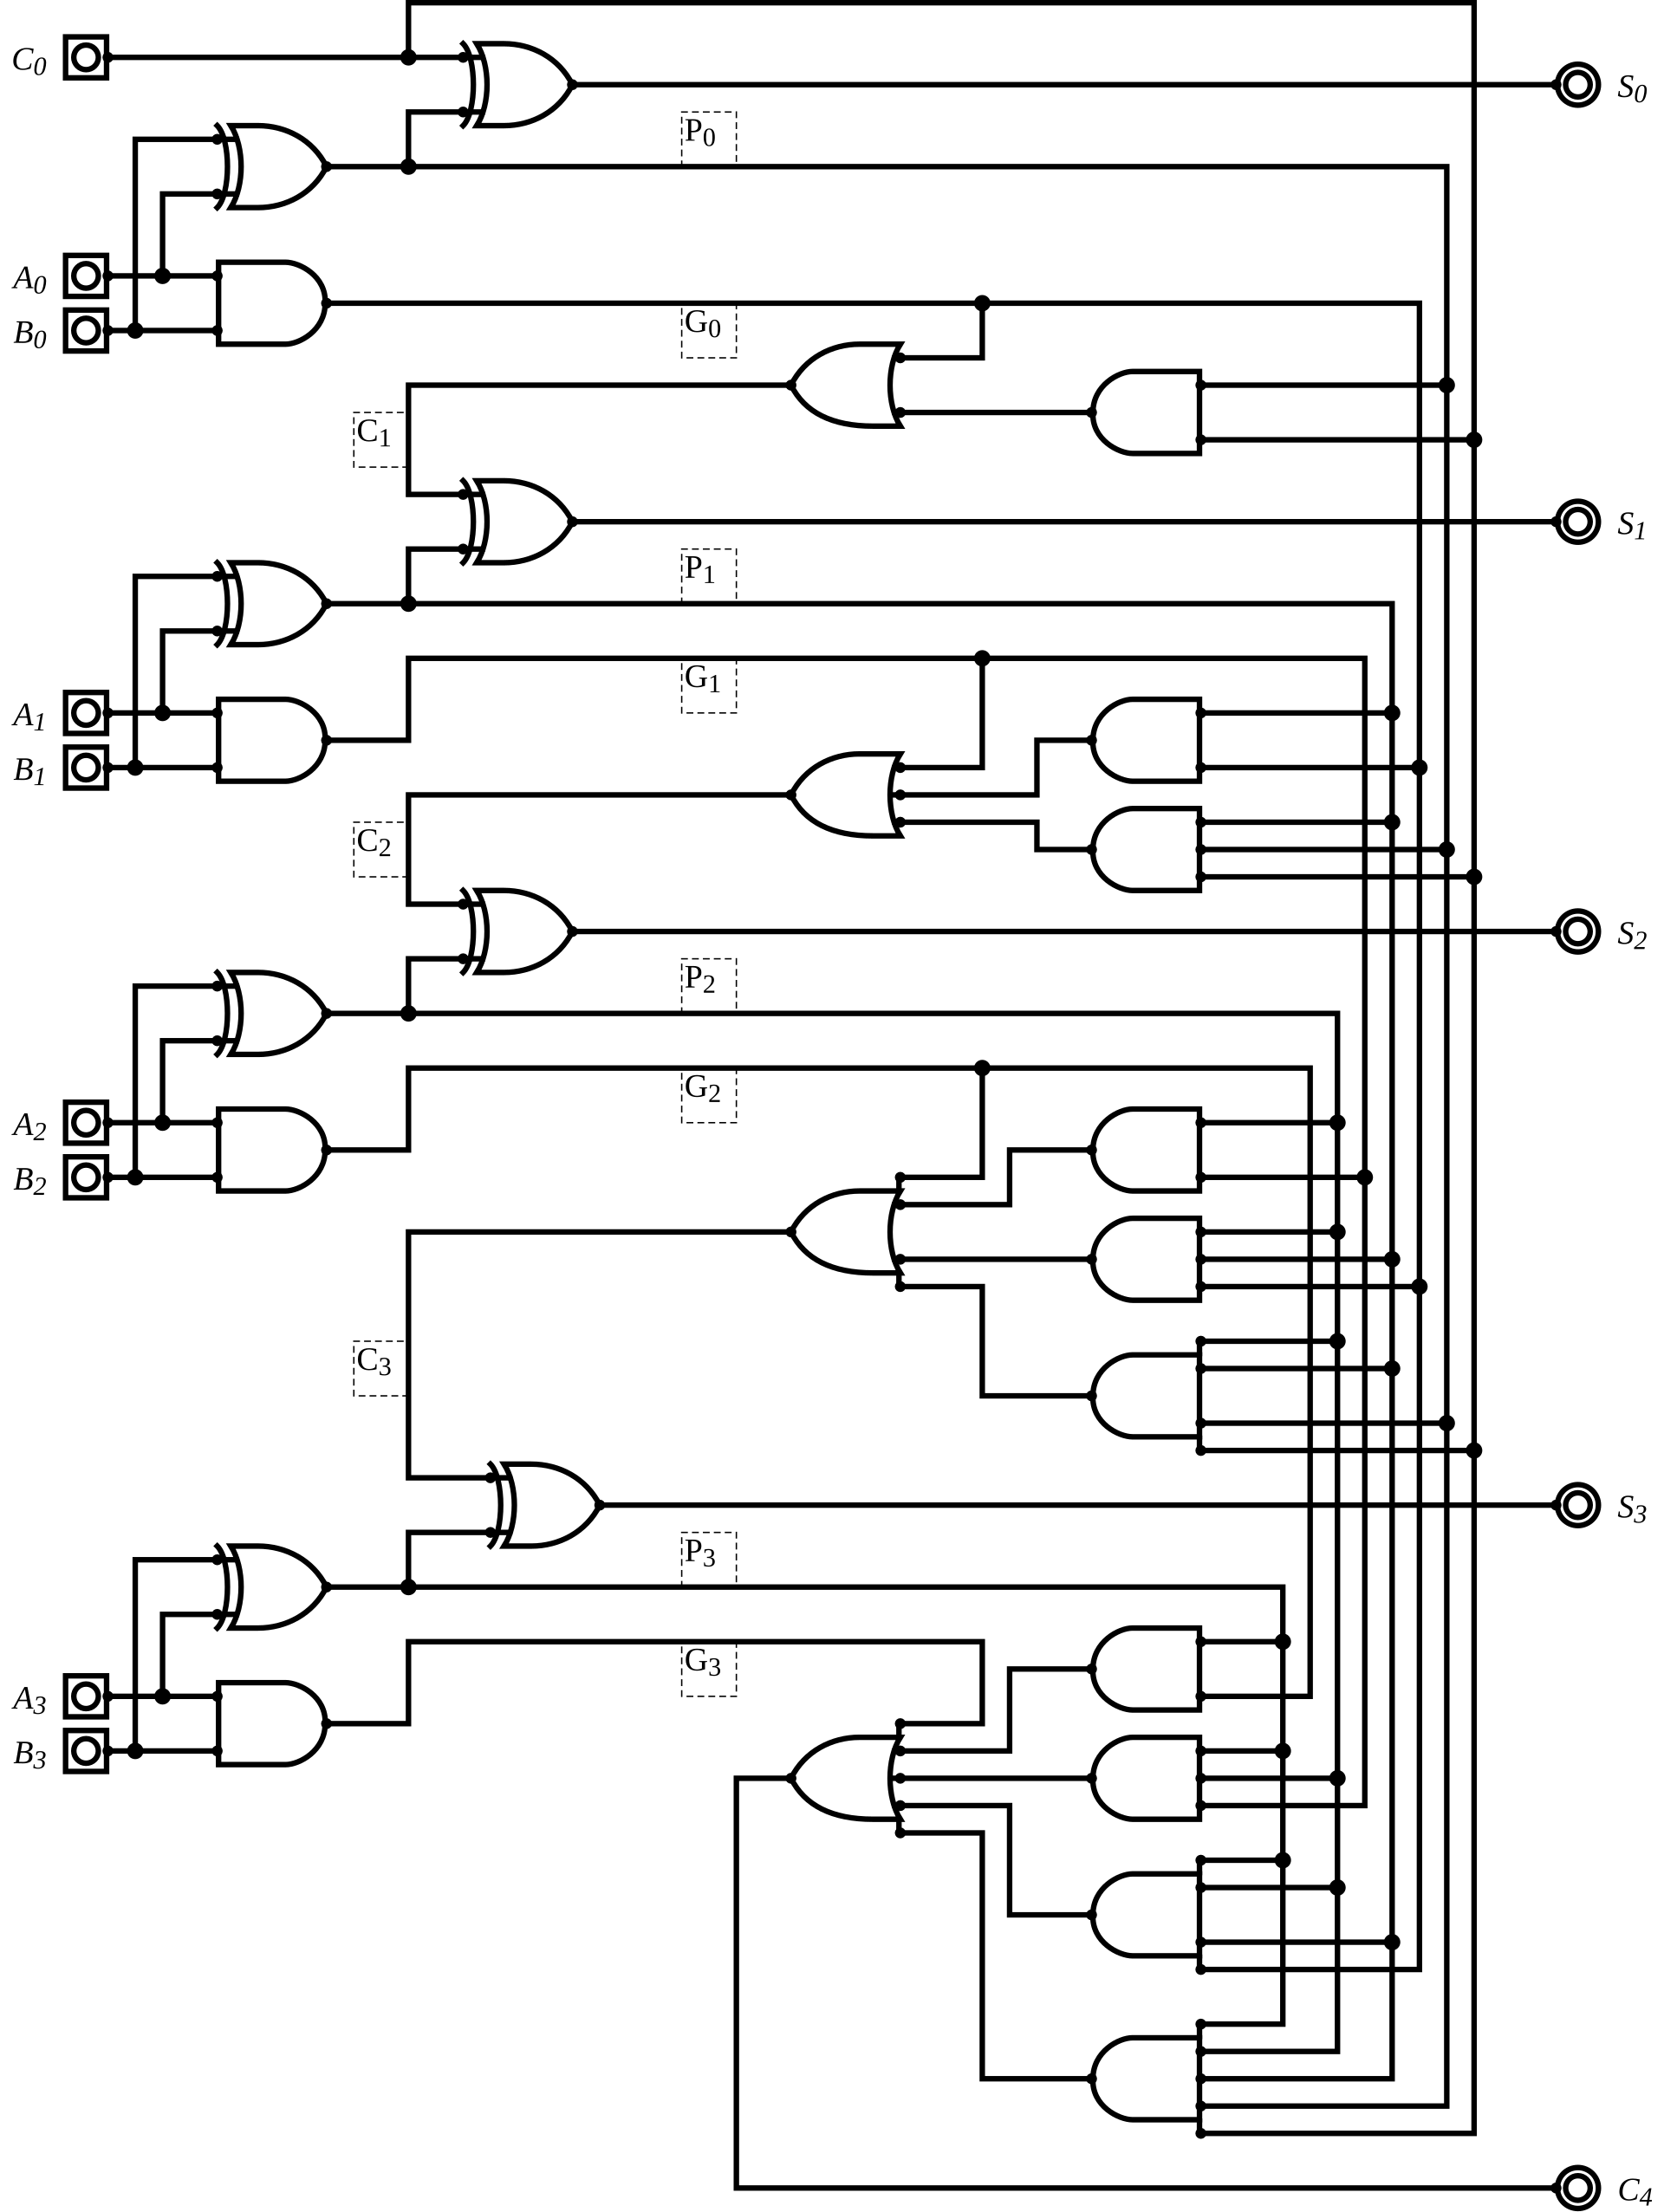
\includegraphics[width=0.4\textwidth]{images/cla_adder_circuit_diagram.png}
    \caption{Circuit Diagram for CLA Adder}
    \label{fig:cla}
\end{figure}


\subsection{D Flip Flop}

\subsubsection{CMOS Implementation}

The obvious and basic choice would be to use CMOS gates to implement the D Flip Flop. This uses two D Latches in a Master-Slave configuration.

\begin{figure}[H]
    \centering
    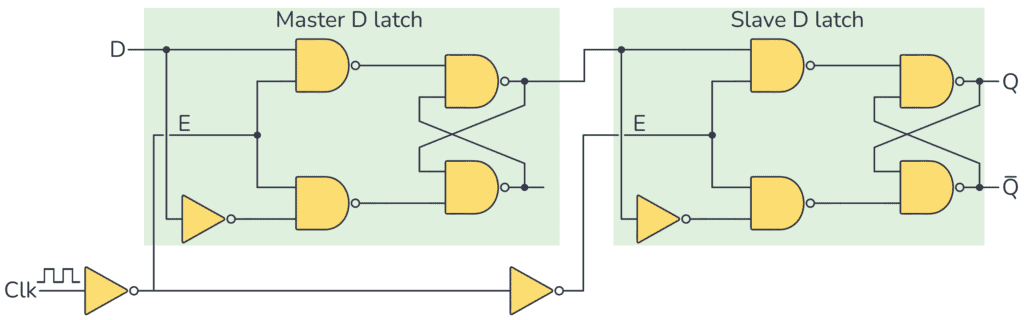
\includegraphics[width=0.4\textwidth]{images/d_ff_cmos_circuit_diagram.png}
    \caption{Circuit Diagram for CMOS D Flip Flop}
\end{figure}

The issues with this circuit are:
\begin{enumerate}
    \item The circuit is slow as it has a large propagation delay.
    \item The circuit has large area, as we will see later in the layout.
\end{enumerate}

\subsubsection{Optimized Implementation}

This circuit works by storing the value of D after the first inverter when the clock signal is low. In the rising edge of the clock, D does not pass through the first MOSFET, and the stored value is passed to the output Q.

\begin{figure}[H]
    \centering
    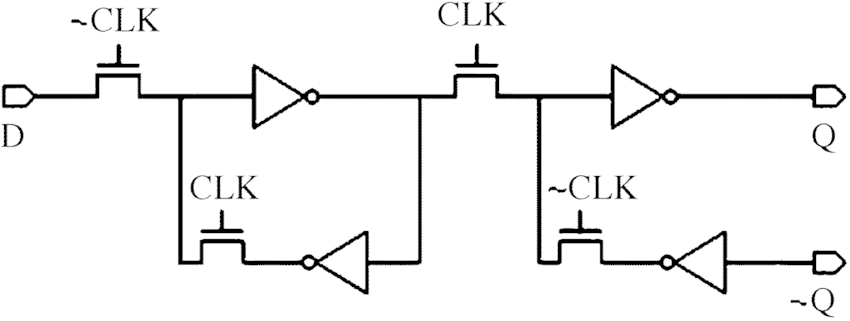
\includegraphics[width=0.4\textwidth]{images/d_ff_circuit_diagram.png}
    \caption{Circuit Diagram for Optimized D Flip Flop}
\end{figure}



\section{Verilog Simulation}

First, we test the digital logic using Verilog simulations. We use GTKWave to plot our results from the testbench. Later, we put this onto an FPGA board to test the circuit in real life.

\begin{figure}[hb]
    \centering
    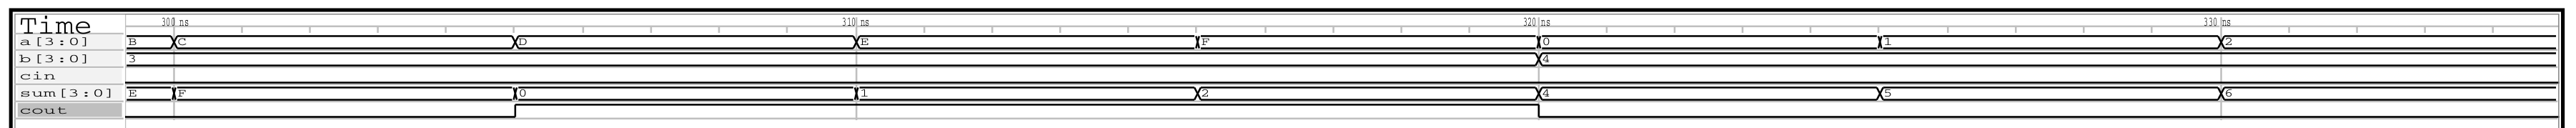
\includegraphics[width=0.48\textwidth]{images/verilog_cla.png}
    \caption{GTKWave Plot of CLA Adder Verilog Simulation}
\end{figure}

\begin{figure}[hb]
    \centering
    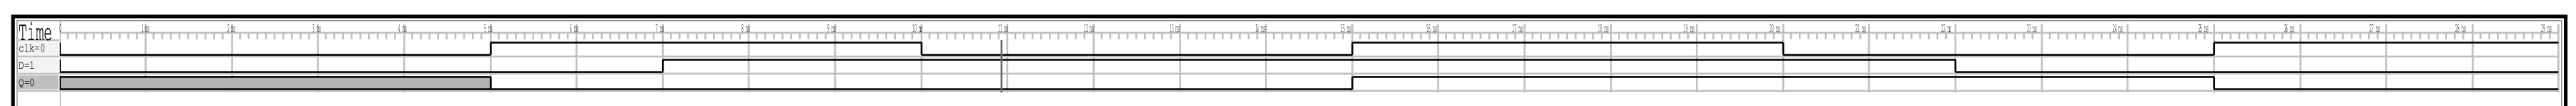
\includegraphics[width=0.48\textwidth]{images/verilog_d_ff.png}
    \caption{GTKWave Plot of  D Flip Flop Verilog Simulation}
\end{figure}

\begin{figure}[hb]
    \centering
    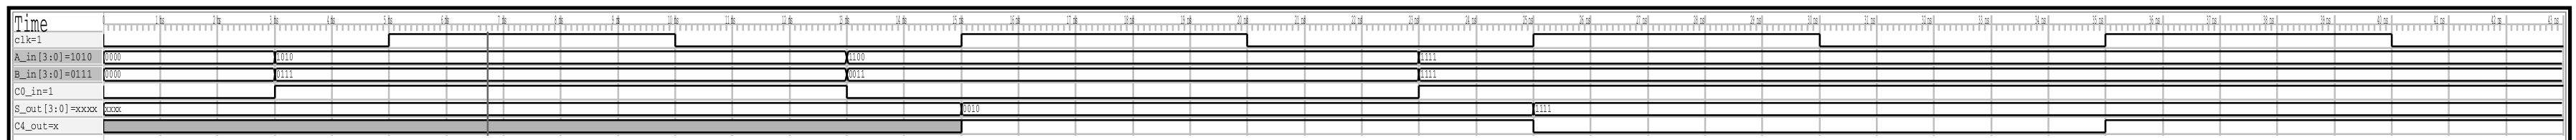
\includegraphics[width=0.48\textwidth]{images/verilog_full.png}
    \caption{GTKWave Plot of Full Circuit Verilog Simulation}
\end{figure}

\section{NGSPICE Simulation}

For all my designs, I've chosen to use a CMOS inverter of $W_p/W_n = 2.5$ as basis. The technology files (180nm) used are included in the repo. \cite{b2}

\subsection{Inverter}

This is the standard CMOS inverter with $W_p/W_n = 2.5$.

\begin{figure}[H]
    \centering
    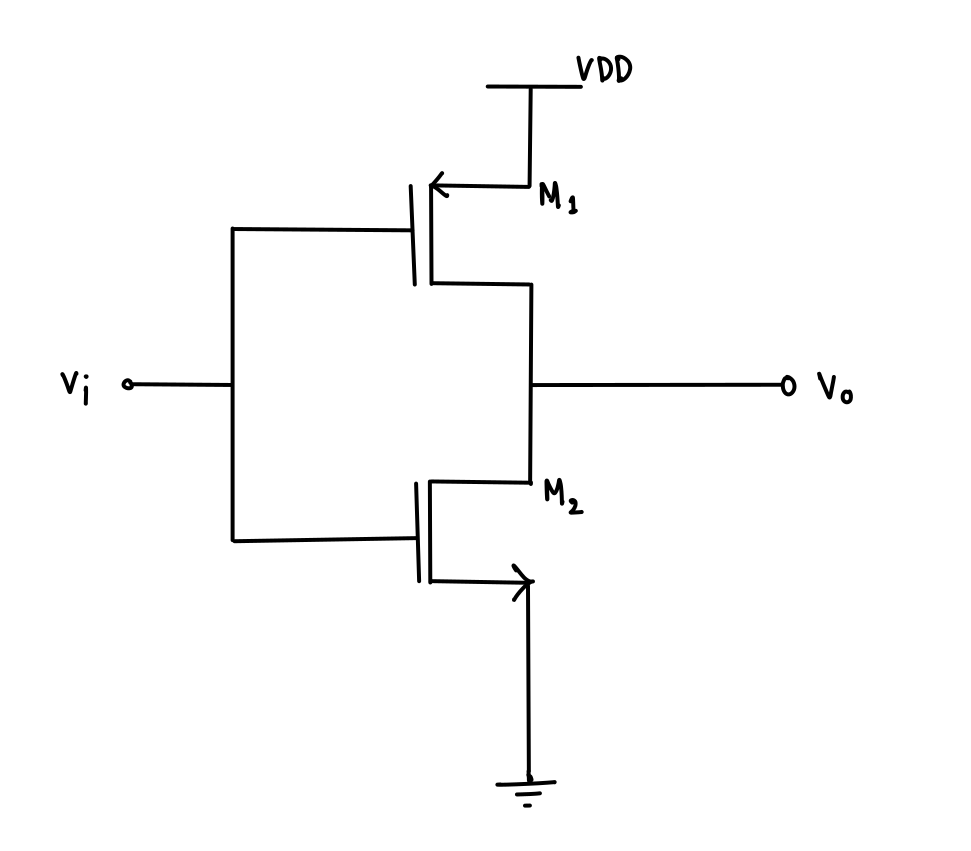
\includegraphics[width=0.48\textwidth]{images/inv_cmos_circuit_diagram.png}
    \caption{Circuit Diagram of Inverter}
\end{figure}

\begin{figure}[H]
    \centering
    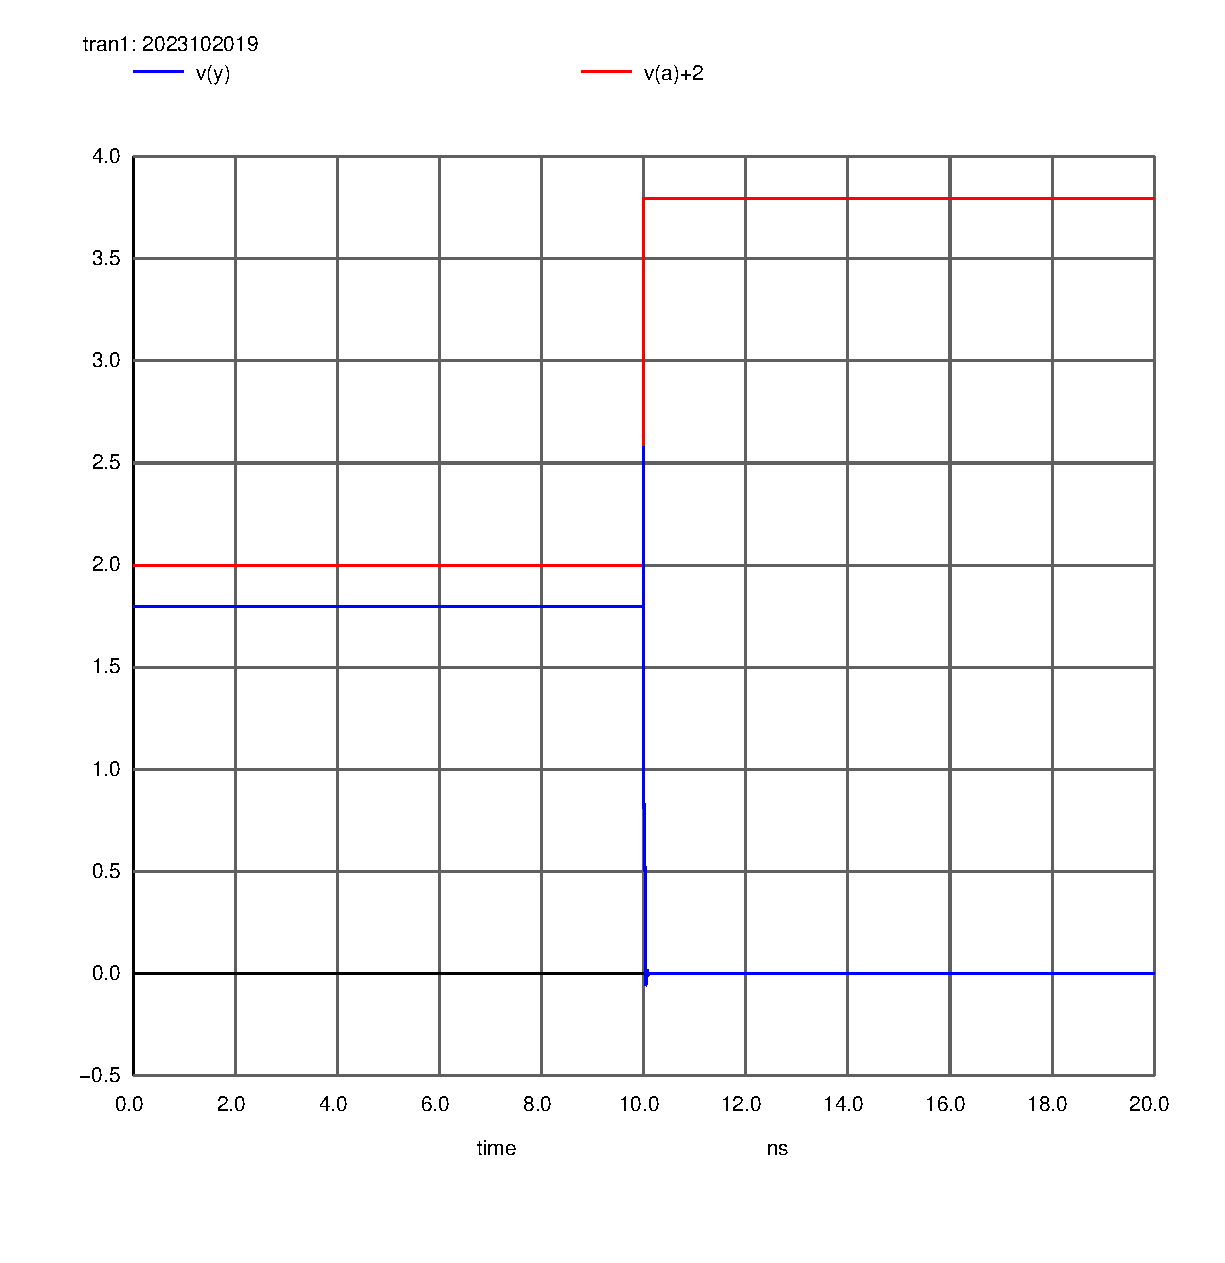
\includegraphics[width=0.48\textwidth]{images/inv_cmos_tran.eps}
    \caption{NGSPICE Plot of Inverter}
\end{figure}

\subsection{NAND Gate}

To size the CMOS NAND gate, we need to equalize the resistance through the Pull-Up network and Pull-Down Network. \\
For an $n$ input NAND gate, where $W_{inv}$ is the size of the NMOS in the inverter:

\begin{align}
    \frac{n}{W_n} &= \frac{1}{W_{inv}} \\
    W_n &= n \cdot W_{inv}
\end{align}

$W_p$ stays the same.

\begin{figure}[H]
    \centering
    \begin{tabular}{cc}
        \begin{subfigure}{0.44\linewidth}
            \centering
            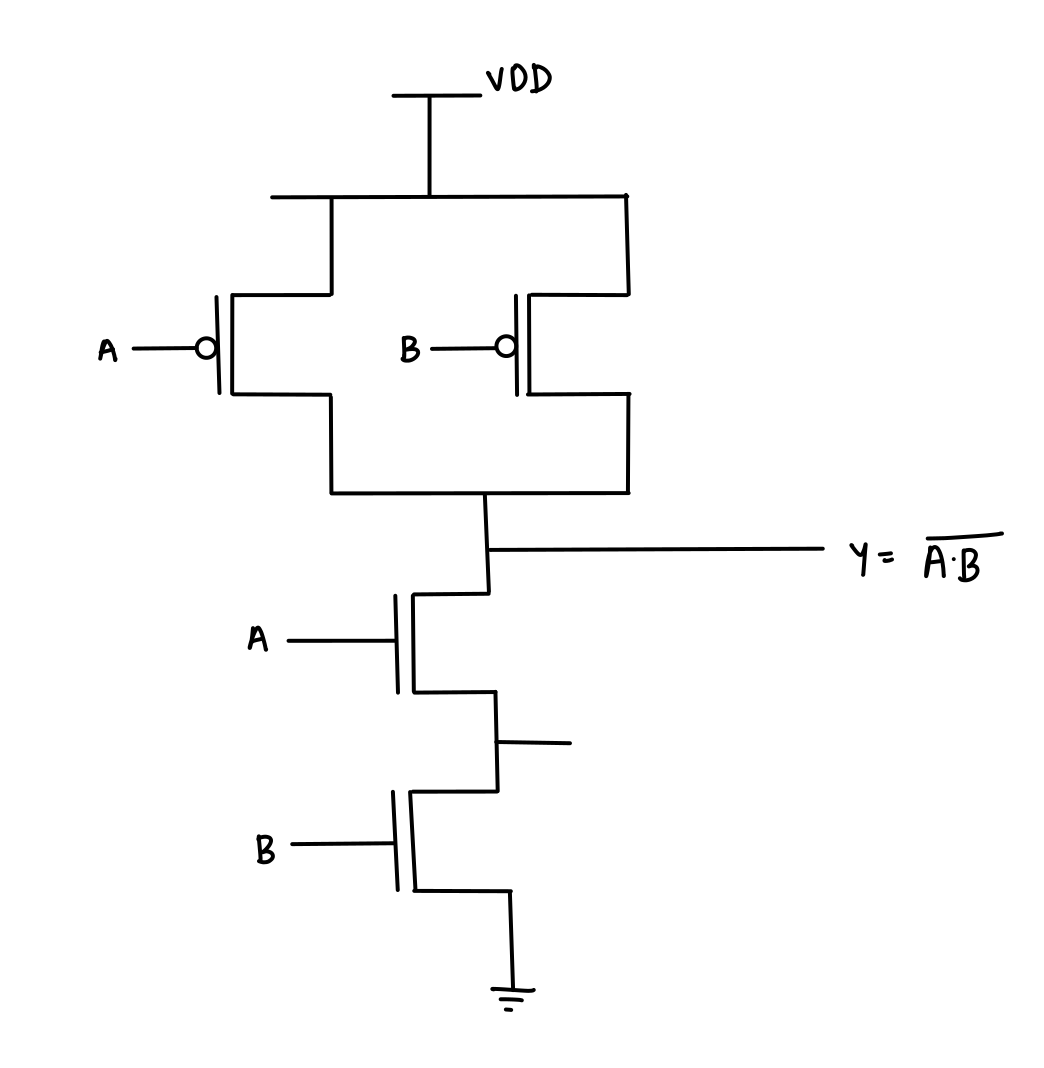
\includegraphics[width=\textwidth]{images/nand_cmos_circuit_diagram.png}
            \caption{2 Input NAND}
        \end{subfigure} &
        \begin{subfigure}{0.44\linewidth}
            \centering
            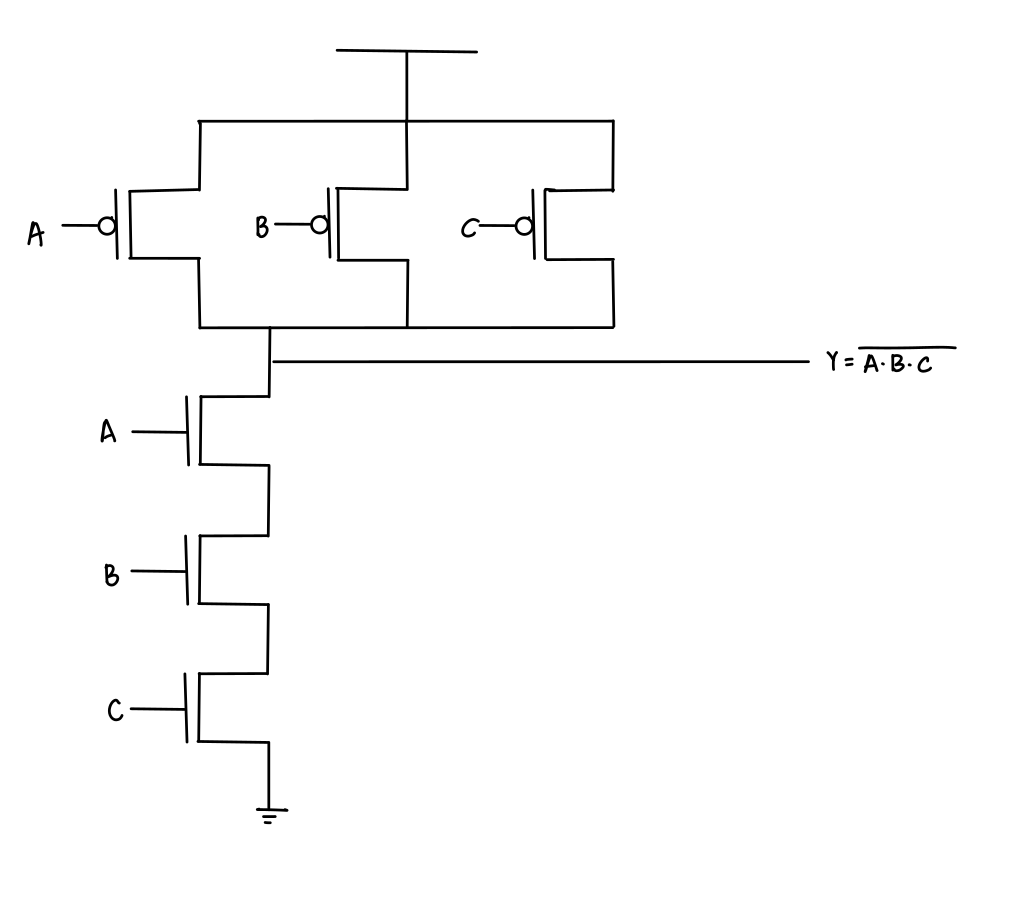
\includegraphics[width=\textwidth]{images/nand_3_cmos_circuit_diagram.png}
            \caption{3 Input NAND}
        \end{subfigure} \\
        \begin{subfigure}{0.44\linewidth}
            \centering
            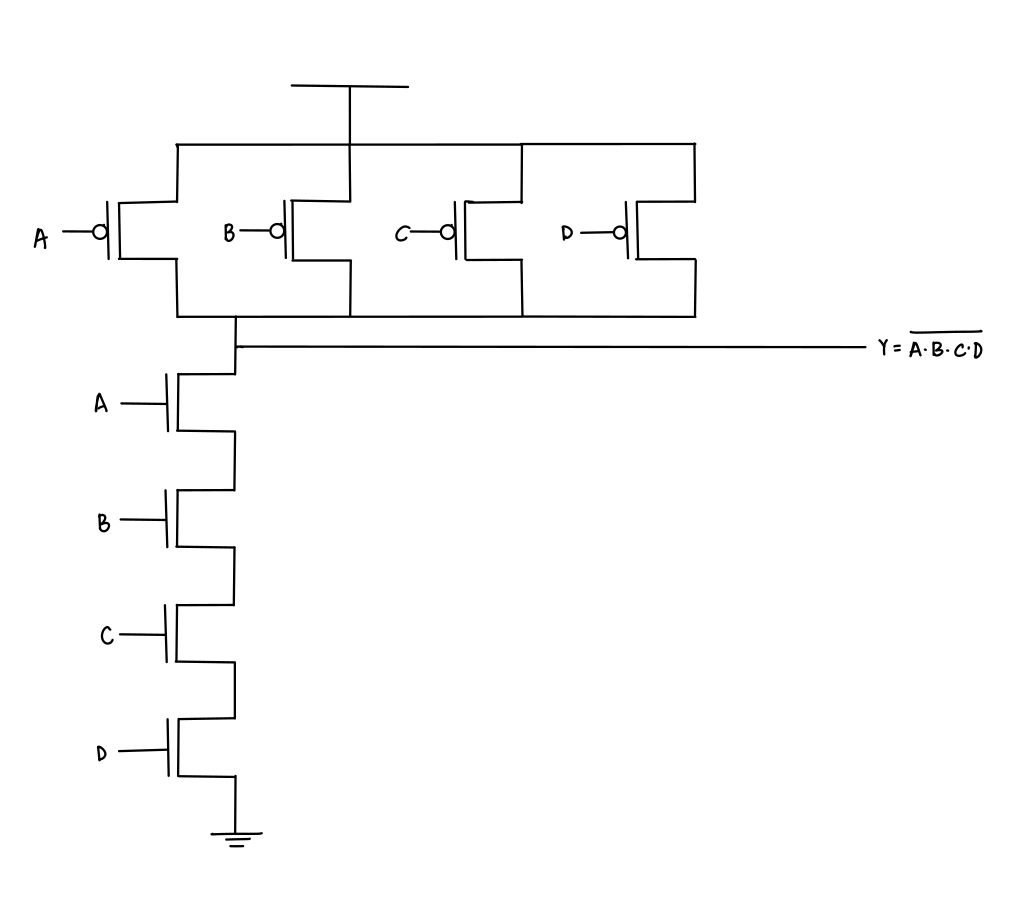
\includegraphics[width=\textwidth]{images/nand_4_cmos_circuit_diagram.png}
            \caption{4 Input NAND}
        \end{subfigure} &
        \begin{subfigure}{0.44\linewidth}
            \centering
            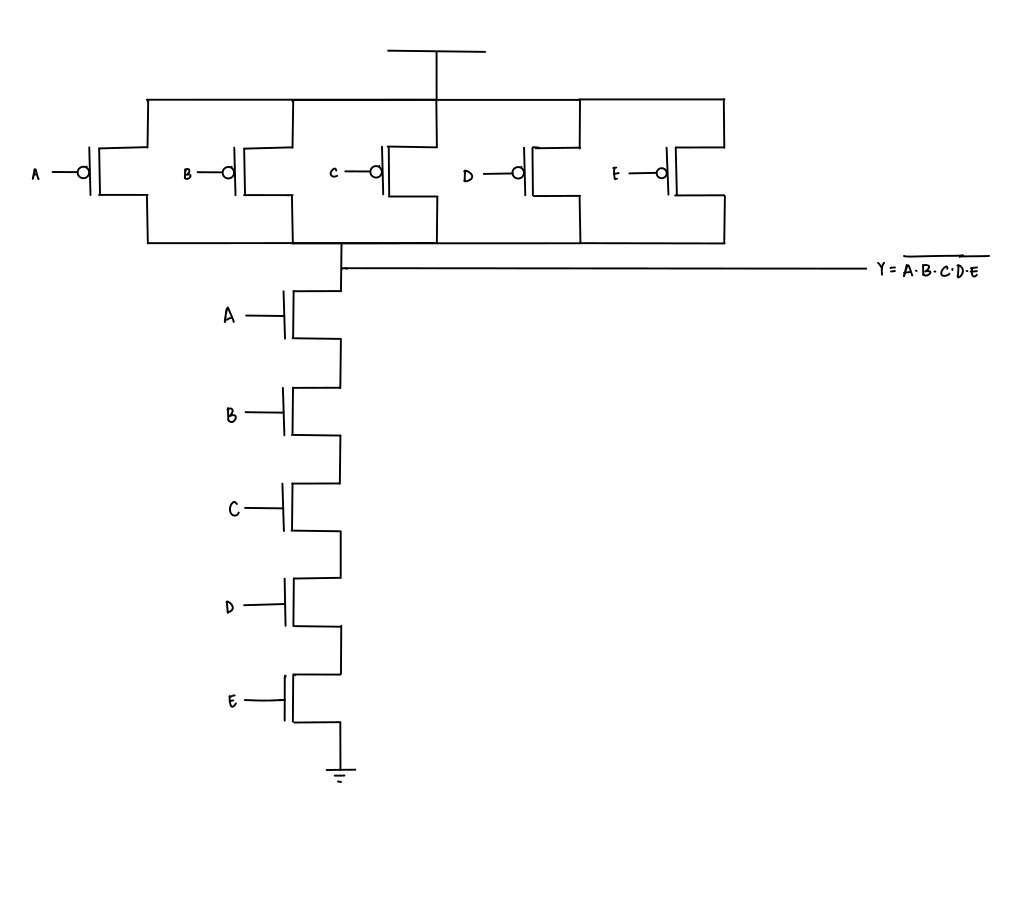
\includegraphics[width=\textwidth]{images/nand_5_cmos_circuit_diagram.png}
            \caption{5 Input NAND}
        \end{subfigure}
    \end{tabular}
    \caption{Circuit Diagram of NAND Gates}
\end{figure}

\begin{figure}[H]
    \centering
    \begin{tabular}{cc}
        \begin{subfigure}{0.44\linewidth}
            \centering
            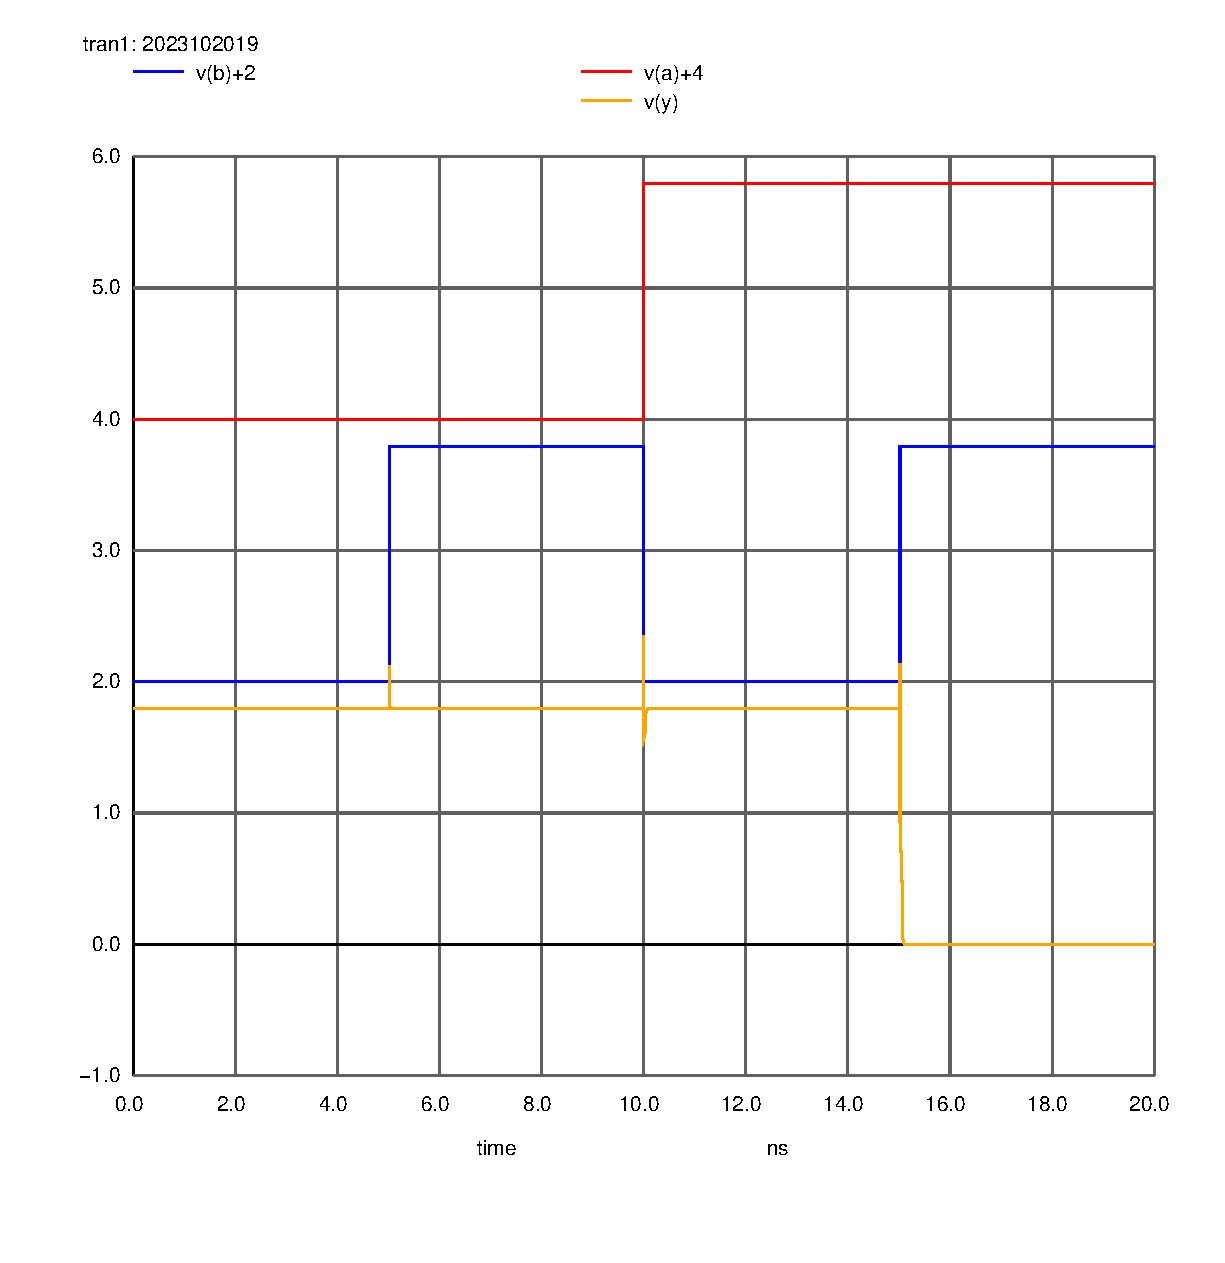
\includegraphics[width=\textwidth]{images/nand_cmos_tran.eps}
            \caption{2 Input NAND}
        \end{subfigure} &
        \begin{subfigure}{0.44\linewidth}
            \centering
            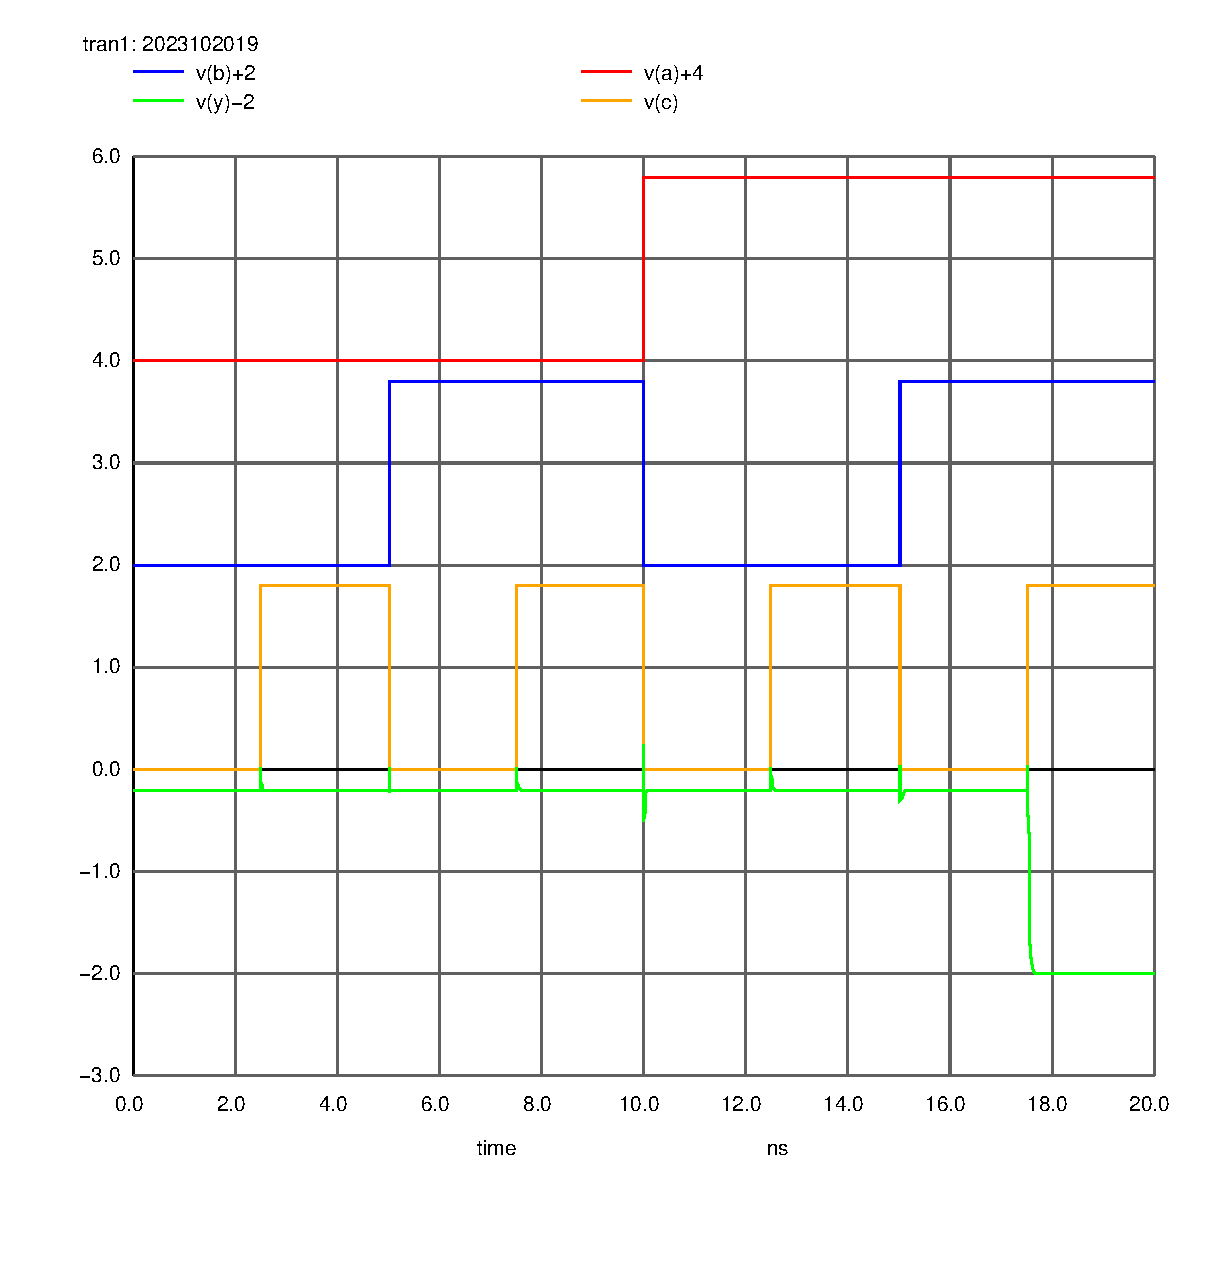
\includegraphics[width=\textwidth]{images/nand_3_cmos_tran.eps}
            \caption{3 Input NAND}
        \end{subfigure} \\
        \begin{subfigure}{0.44\linewidth}
            \centering
            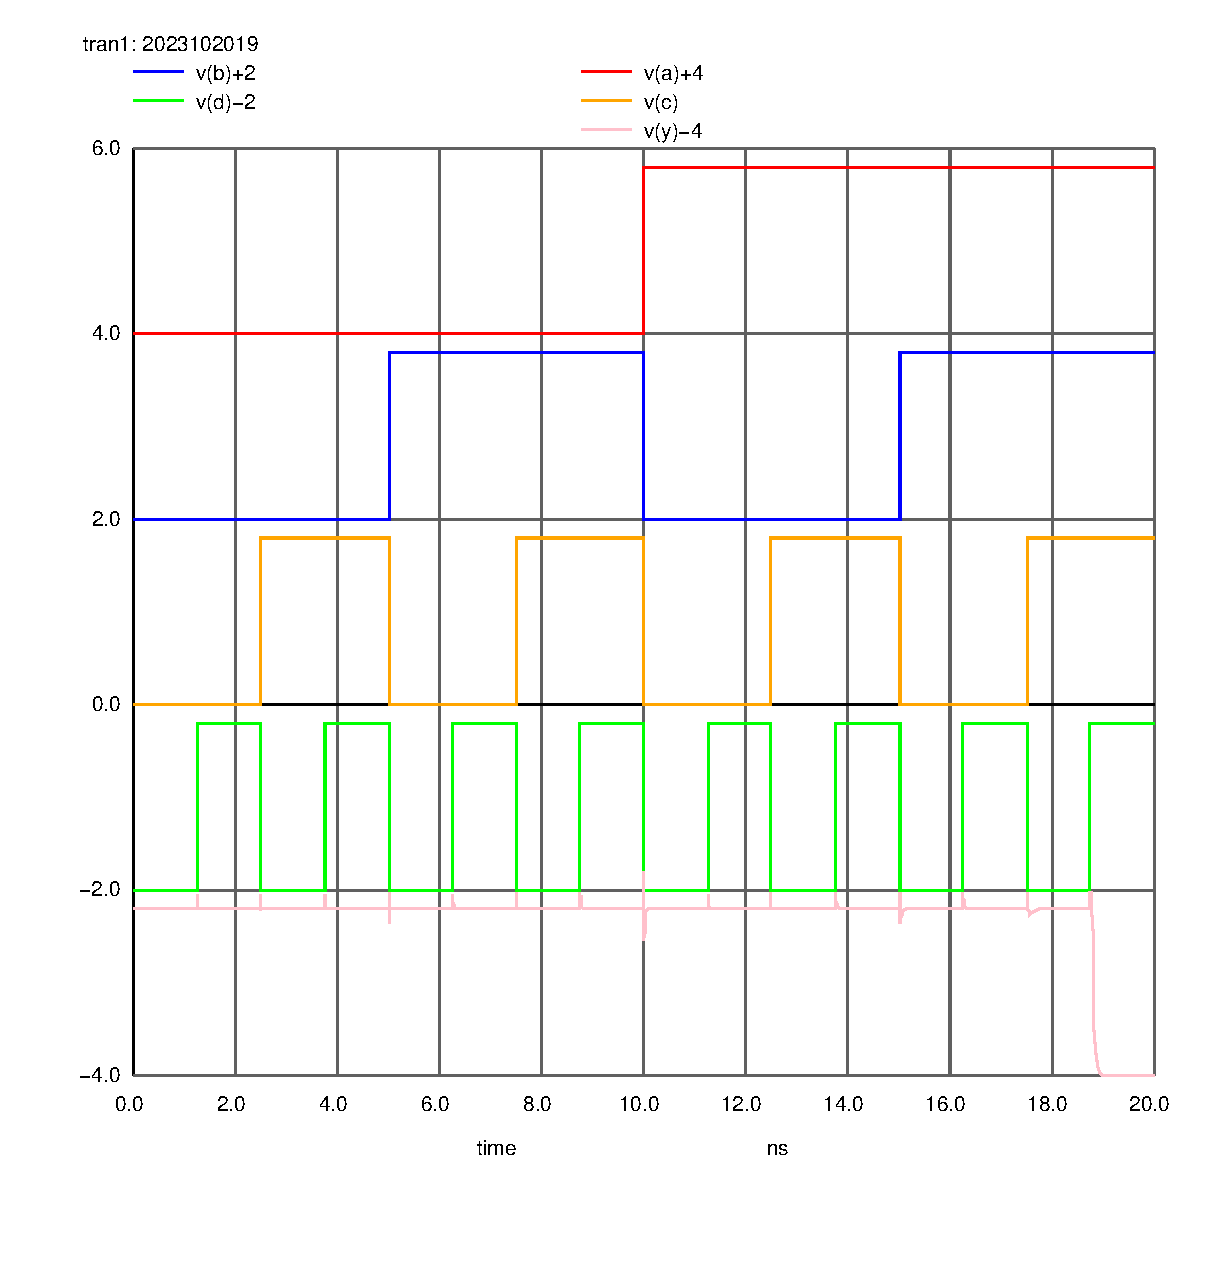
\includegraphics[width=\textwidth]{images/nand_4_cmos_tran.eps}
            \caption{4 Input NAND}
        \end{subfigure} &
        \begin{subfigure}{0.44\linewidth}
            \centering
            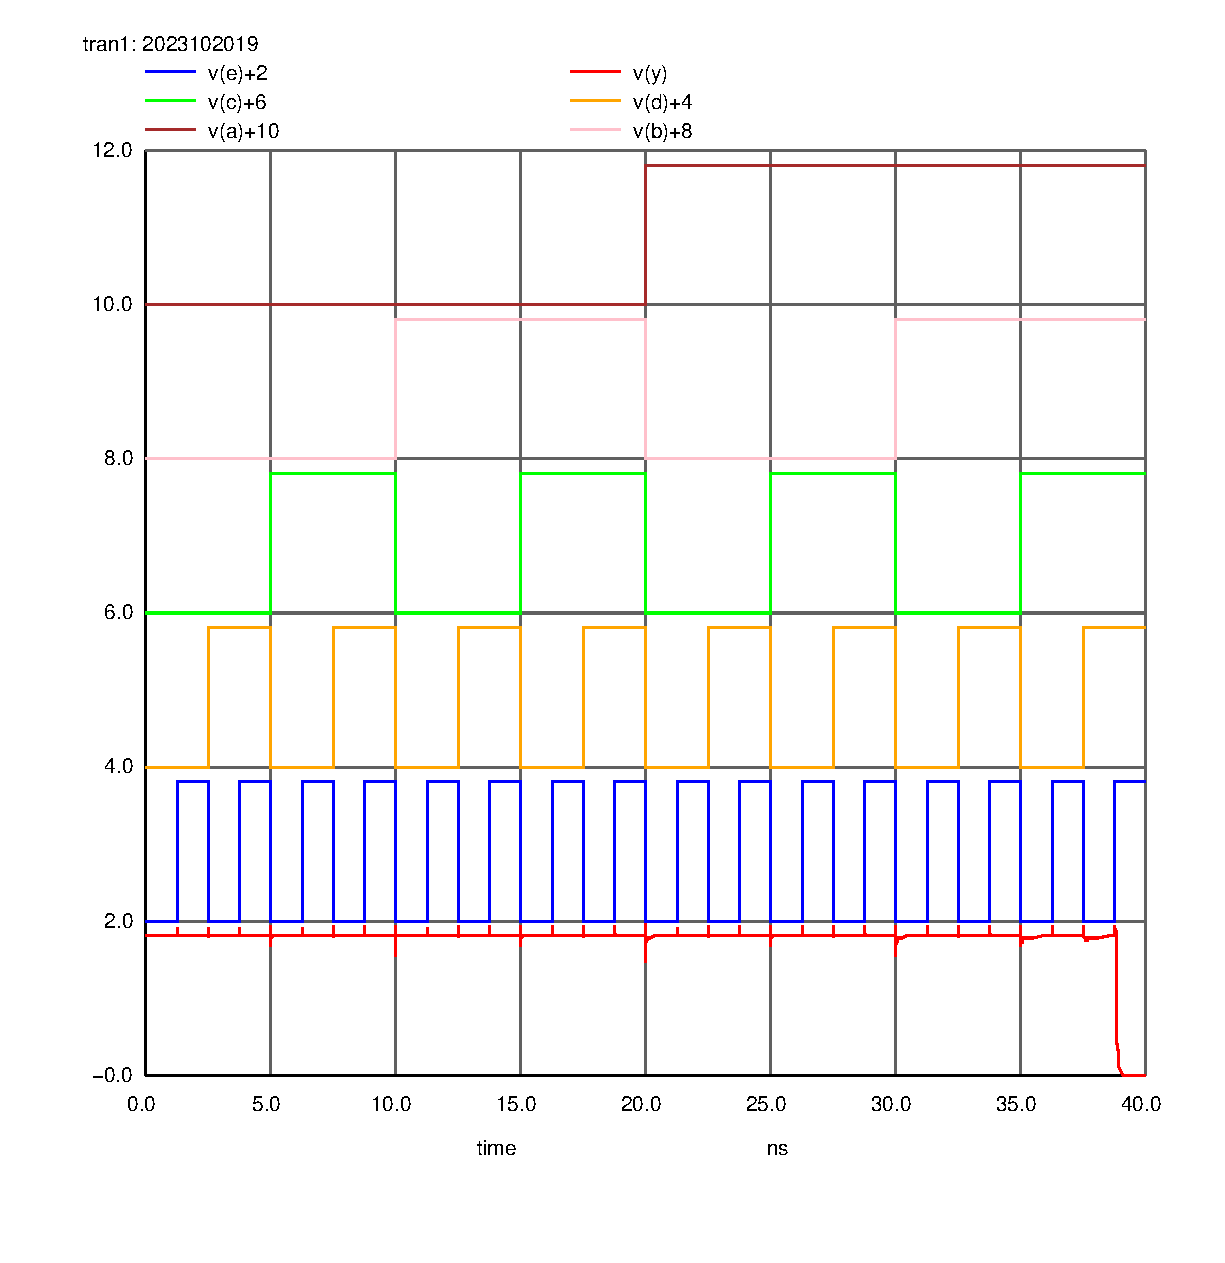
\includegraphics[width=\textwidth]{images/nand_5_cmos_tran.eps}
            \caption{5 Input NAND}
        \end{subfigure}
    \end{tabular}
    \caption{NGSPICE Plot of NAND Gates}
\end{figure}

\subsection{NOR Gate}

Similarly, for the CMOS NOR gate, we need to equalize the resistance through the Pull-Up network and Pull-Down Network. \\
For an $n$ input NOR gate, where $W_{inv}$ is the size of the NMOS in the inverter:

\begin{align}
    \frac{n}{W_p} &= \frac{1}{2.5 \cdot W_{inv}} \\
    W_p &= 2.5  n \cdot W_{inv}
\end{align}

$W_p$ stays the same.

\begin{figure}[H]
    \centering
    \begin{tabular}{cc}
        \begin{subfigure}{0.44\linewidth}
            \centering
            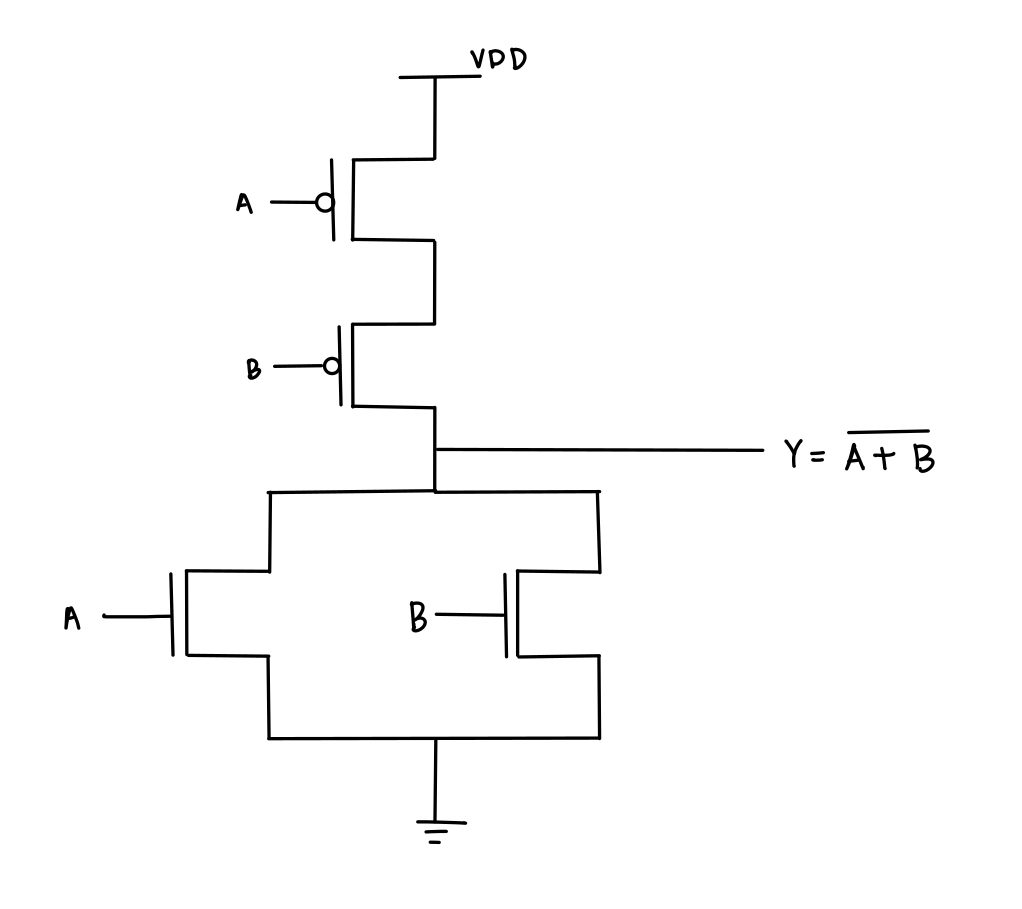
\includegraphics[width=\textwidth]{images/nor_cmos_circuit_diagram.png}
            \caption{2 Input NOR}
        \end{subfigure} &
        \begin{subfigure}{0.44\linewidth}
            \centering
            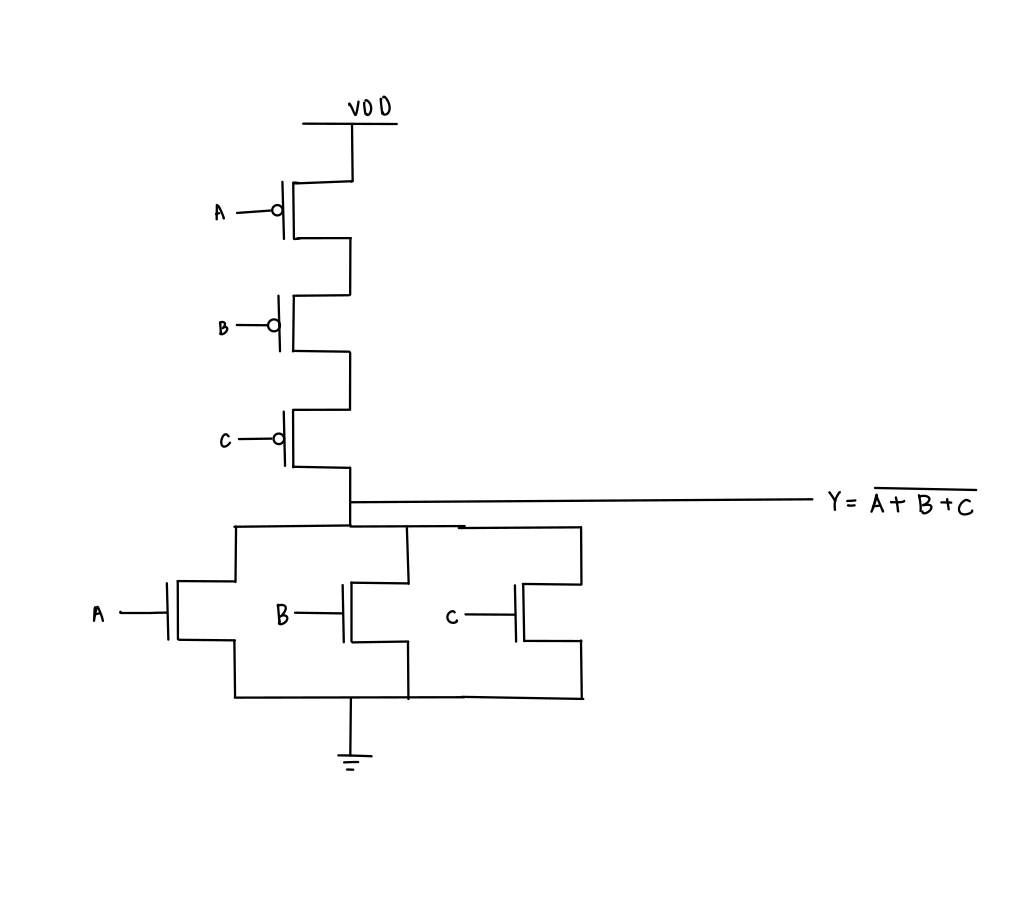
\includegraphics[width=\textwidth]{images/nor_3_cmos_circuit_diagram.png}
            \caption{3 Input NOR}
        \end{subfigure} \\
        \begin{subfigure}{0.44\linewidth}
            \centering
            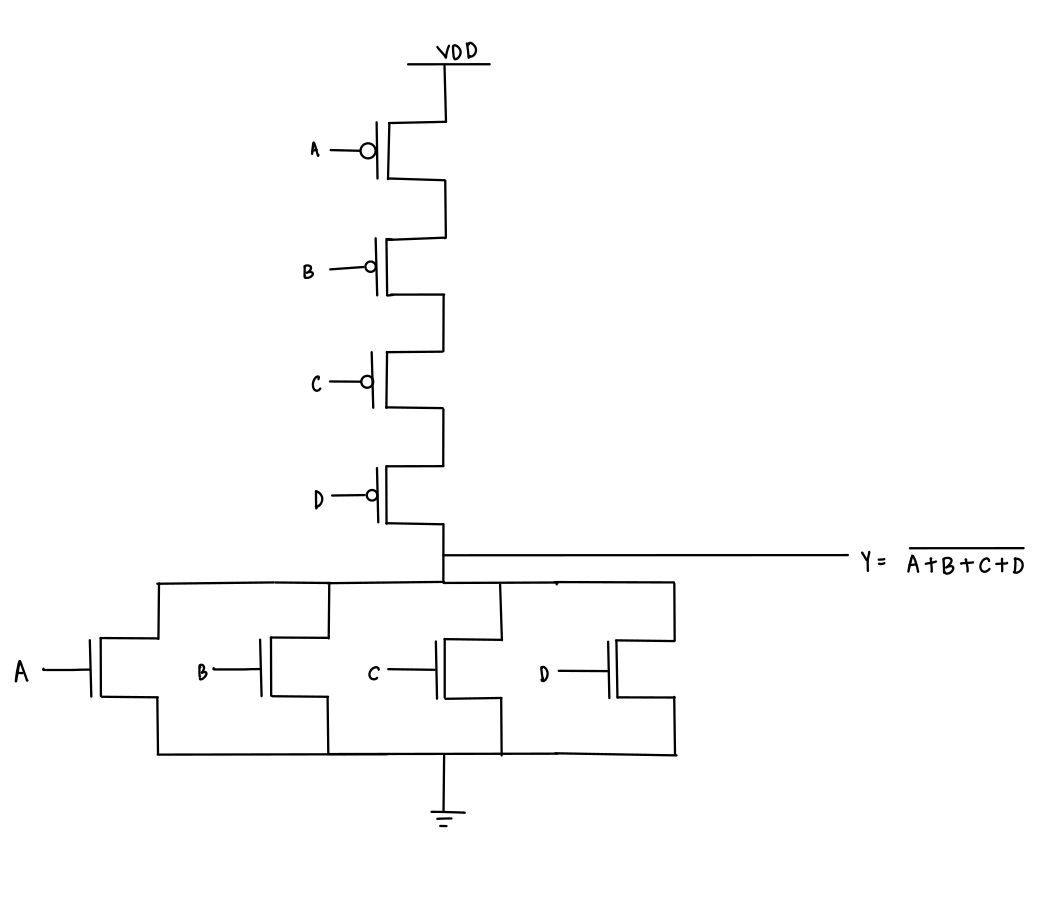
\includegraphics[width=\textwidth]{images/nor_4_cmos_circuit_diagram.png}
            \caption{4 Input NOR}
        \end{subfigure} &
        \begin{subfigure}{0.44\linewidth}
            \centering
            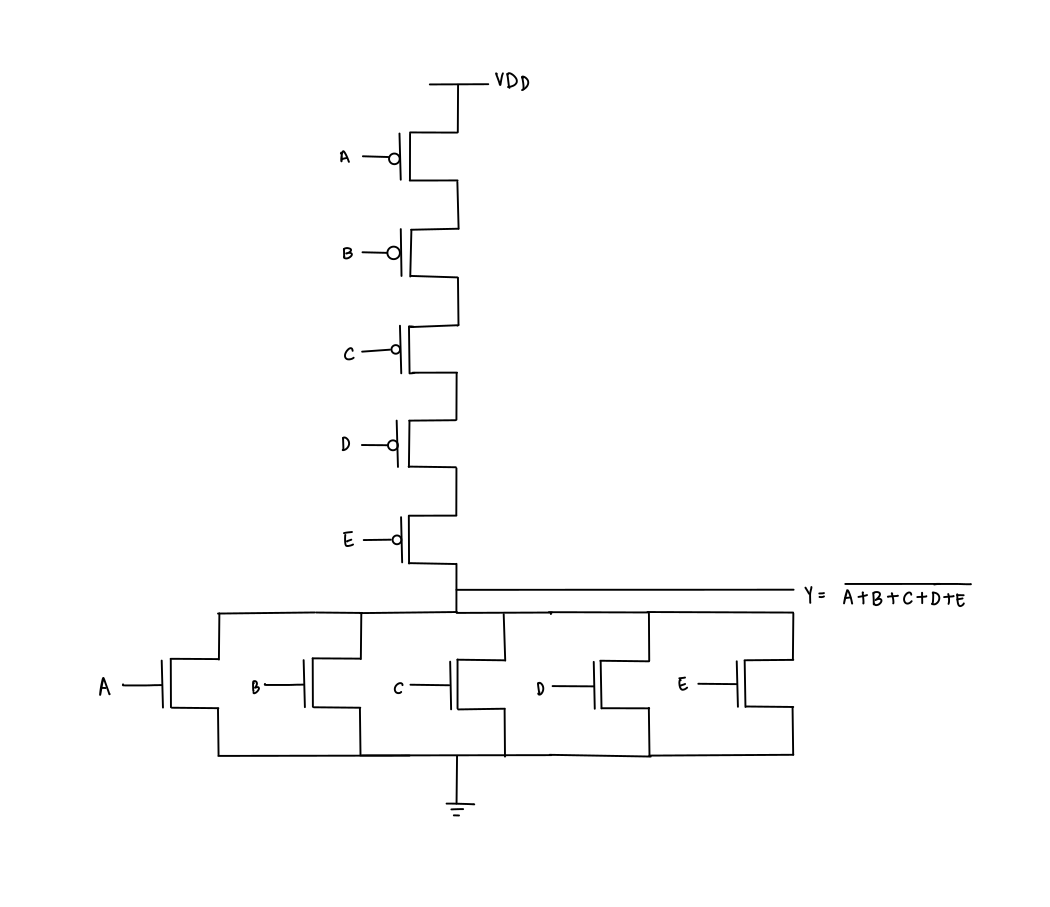
\includegraphics[width=\textwidth]{images/nor_5_cmos_circuit_diagram.png}
            \caption{5 Input NOR}
        \end{subfigure}
    \end{tabular}
    \caption{Circuit Diagram of NOR Gates}
\end{figure}

\begin{figure}[H]
    \centering
    \begin{tabular}{cc}
        \begin{subfigure}{0.44\linewidth}
            \centering
            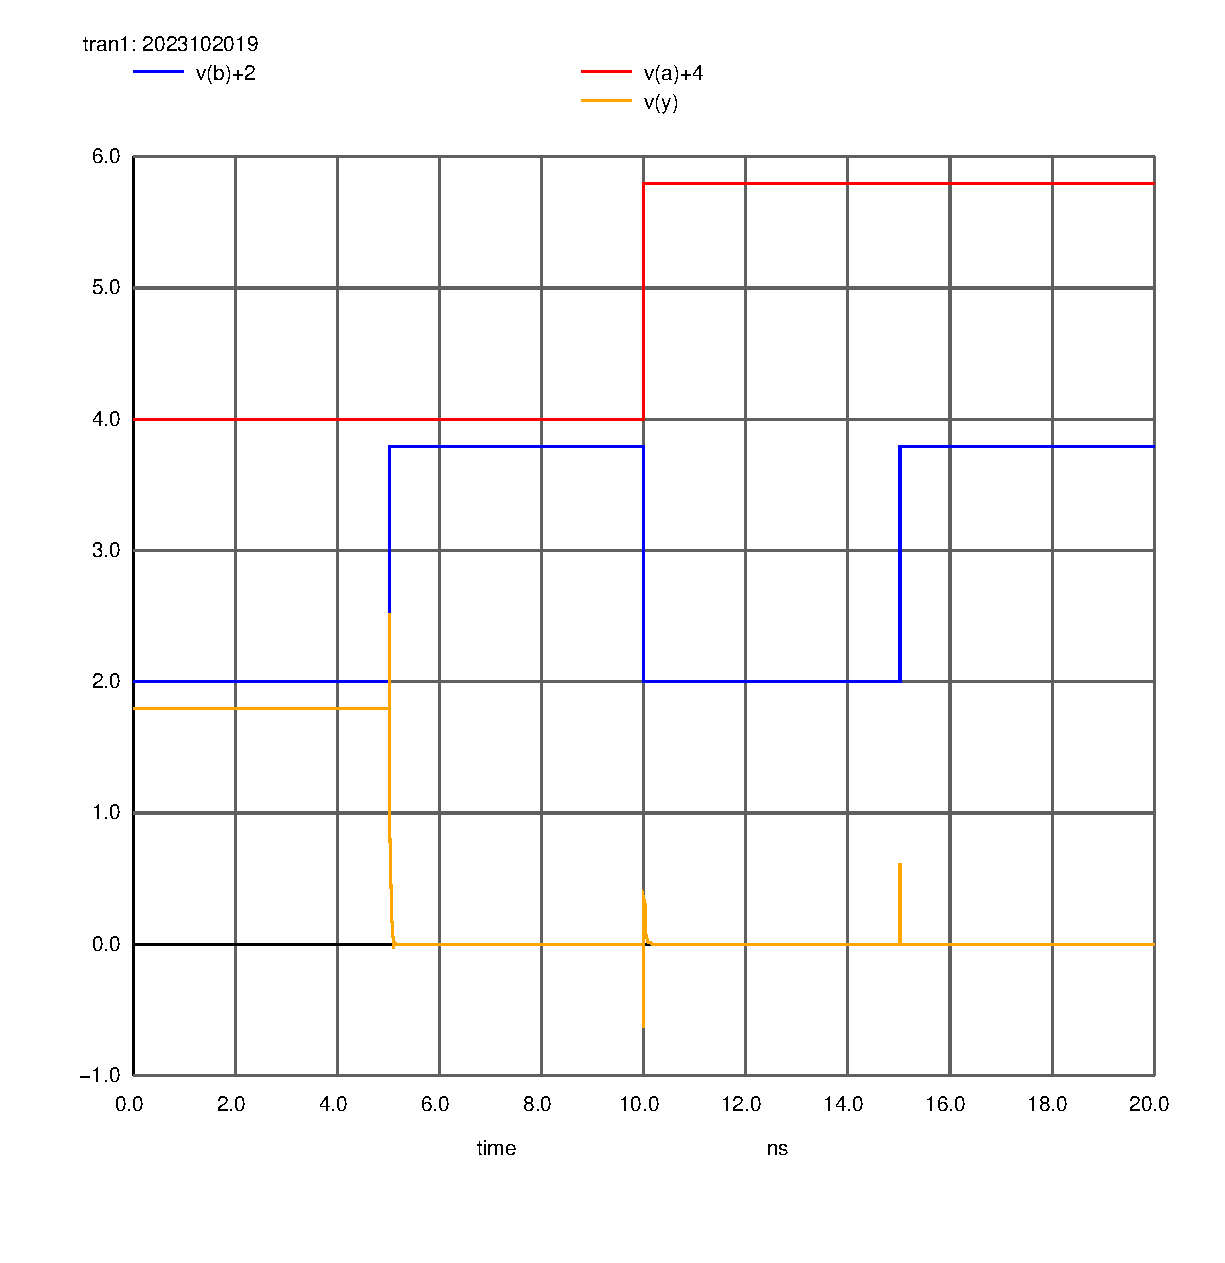
\includegraphics[width=\textwidth]{images/nor_cmos_tran.eps}
            \caption{2 Input NOR}
        \end{subfigure} &
        \begin{subfigure}{0.44\linewidth}
            \centering
            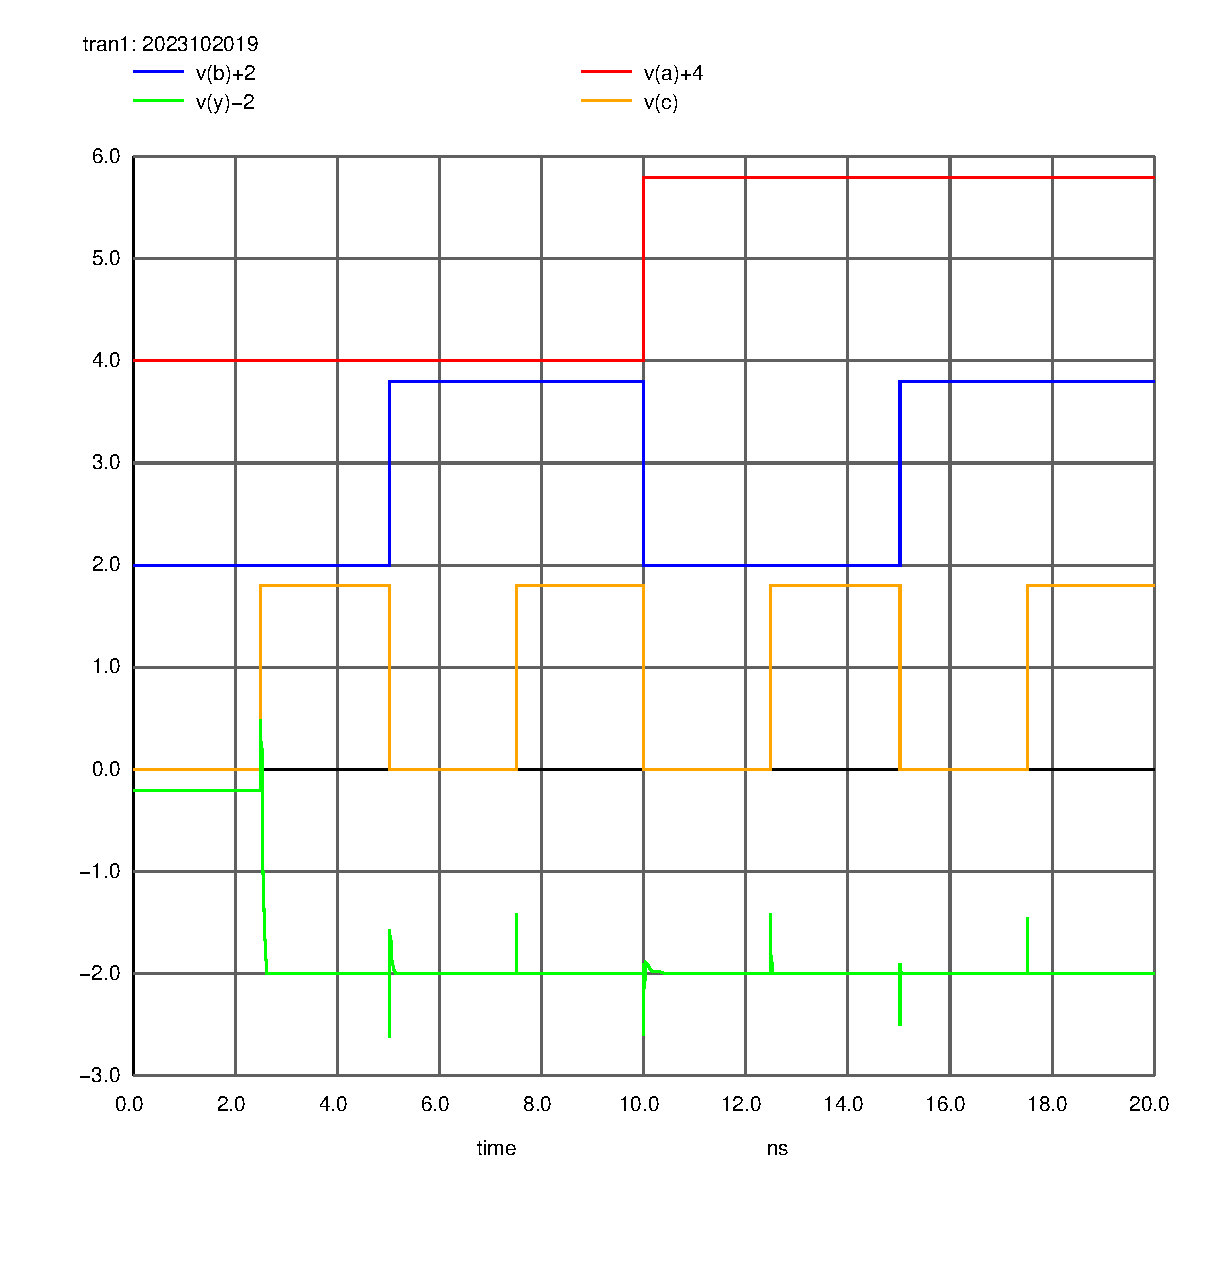
\includegraphics[width=\textwidth]{images/nor_3_cmos_tran.eps}
            \caption{3 Input NOR}
        \end{subfigure} \\
        \begin{subfigure}{0.44\linewidth}
            \centering
            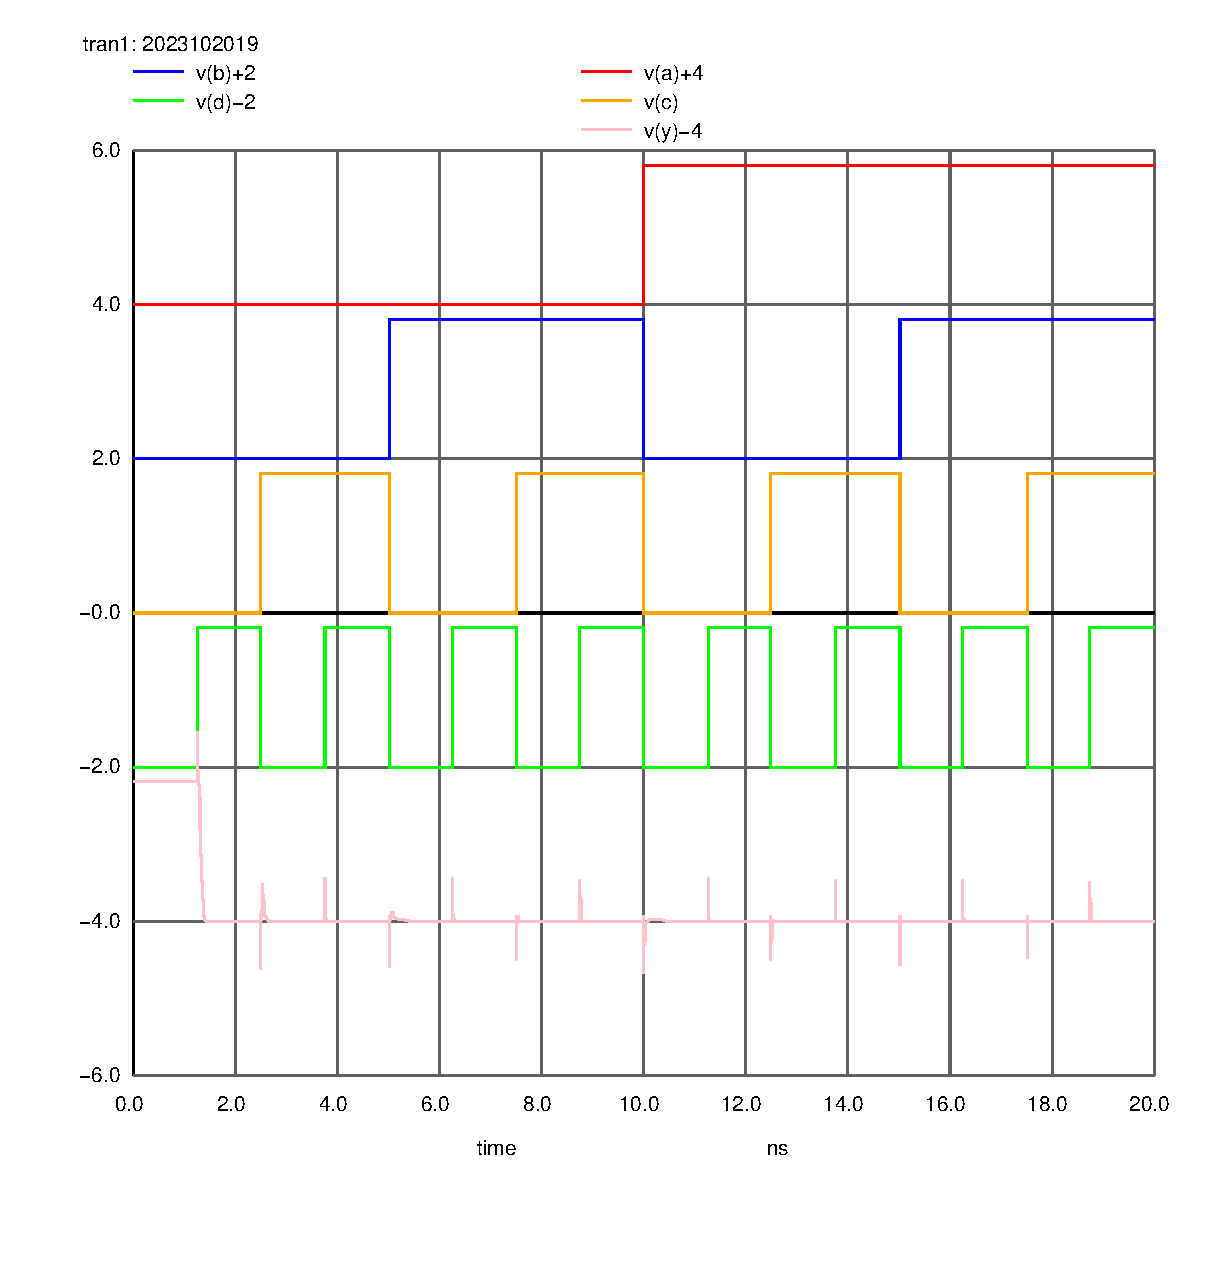
\includegraphics[width=\textwidth]{images/nor_4_cmos_tran.eps}
            \caption{4 Input NOR}
        \end{subfigure} &
        \begin{subfigure}{0.44\linewidth}
            \centering
            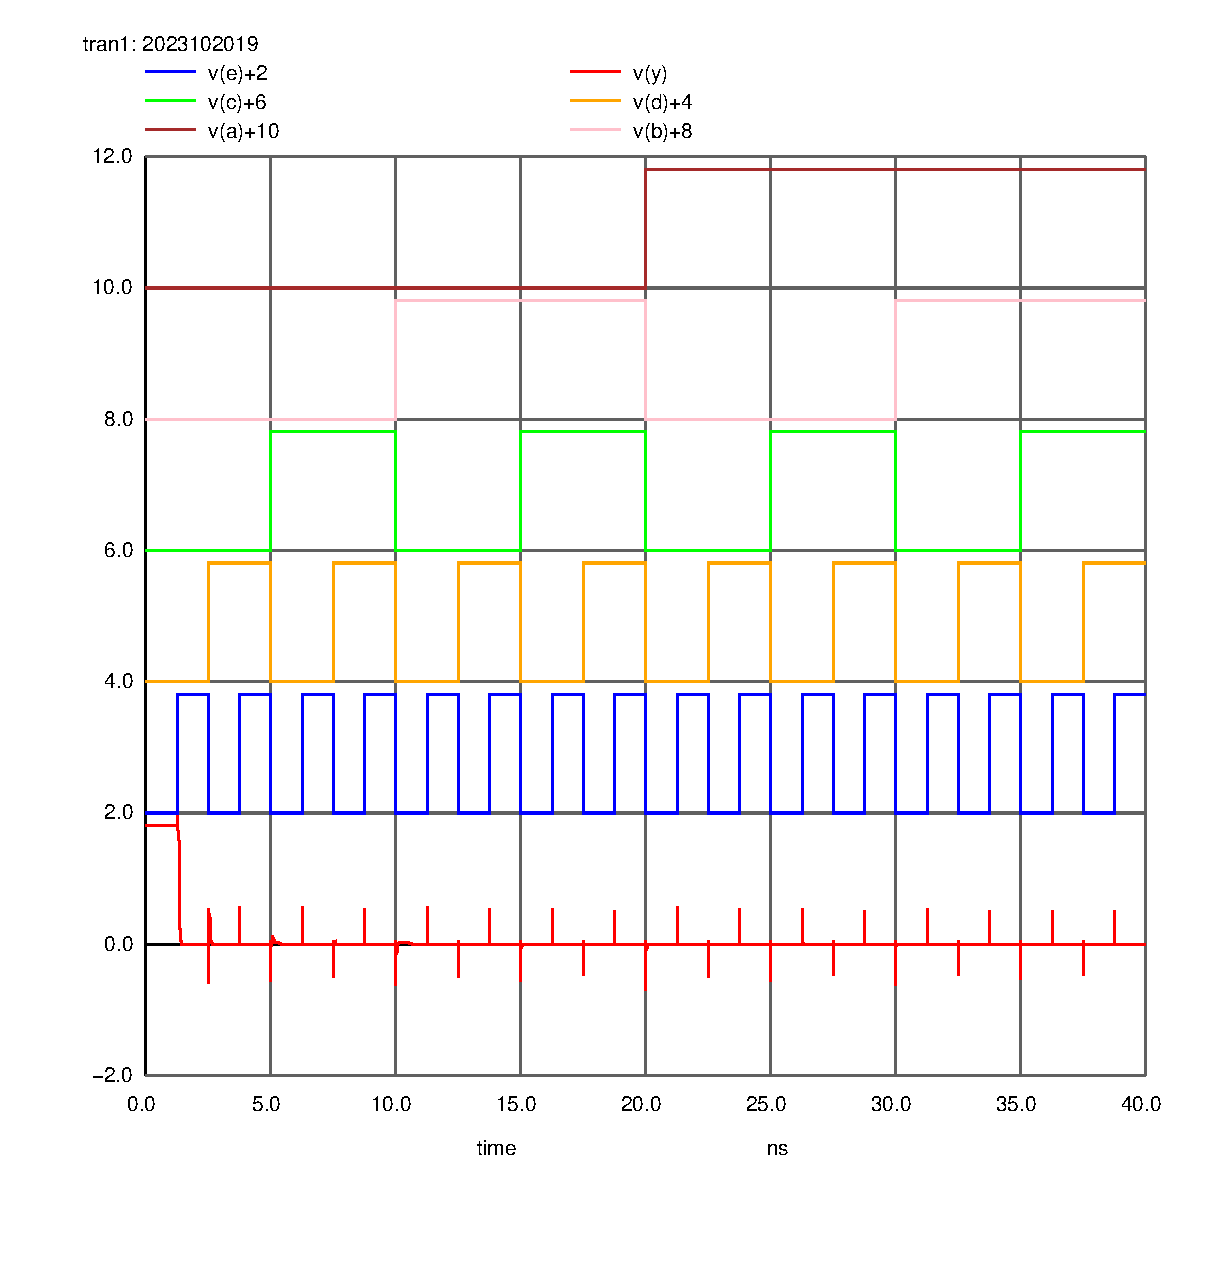
\includegraphics[width=\textwidth]{images/nor_5_cmos_tran.eps}
            \caption{5 Input NOR}
        \end{subfigure}
    \end{tabular}
    \caption{NGSPICE Plot of NOR Gates}
\end{figure}

\subsection{XOR Gate}

\subsubsection{CMOS Implementation}

The standard CMOS Implementation works, but we can do better with less gates.

\begin{figure}[H]
    \centering
    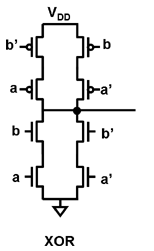
\includegraphics[width=0.2\textwidth]{images/xor_cmos_circuit_diagram.png}
    \caption{Circuit Diagram of CMOS XOR Gate}
\end{figure}

\begin{figure}[H]
    \centering
    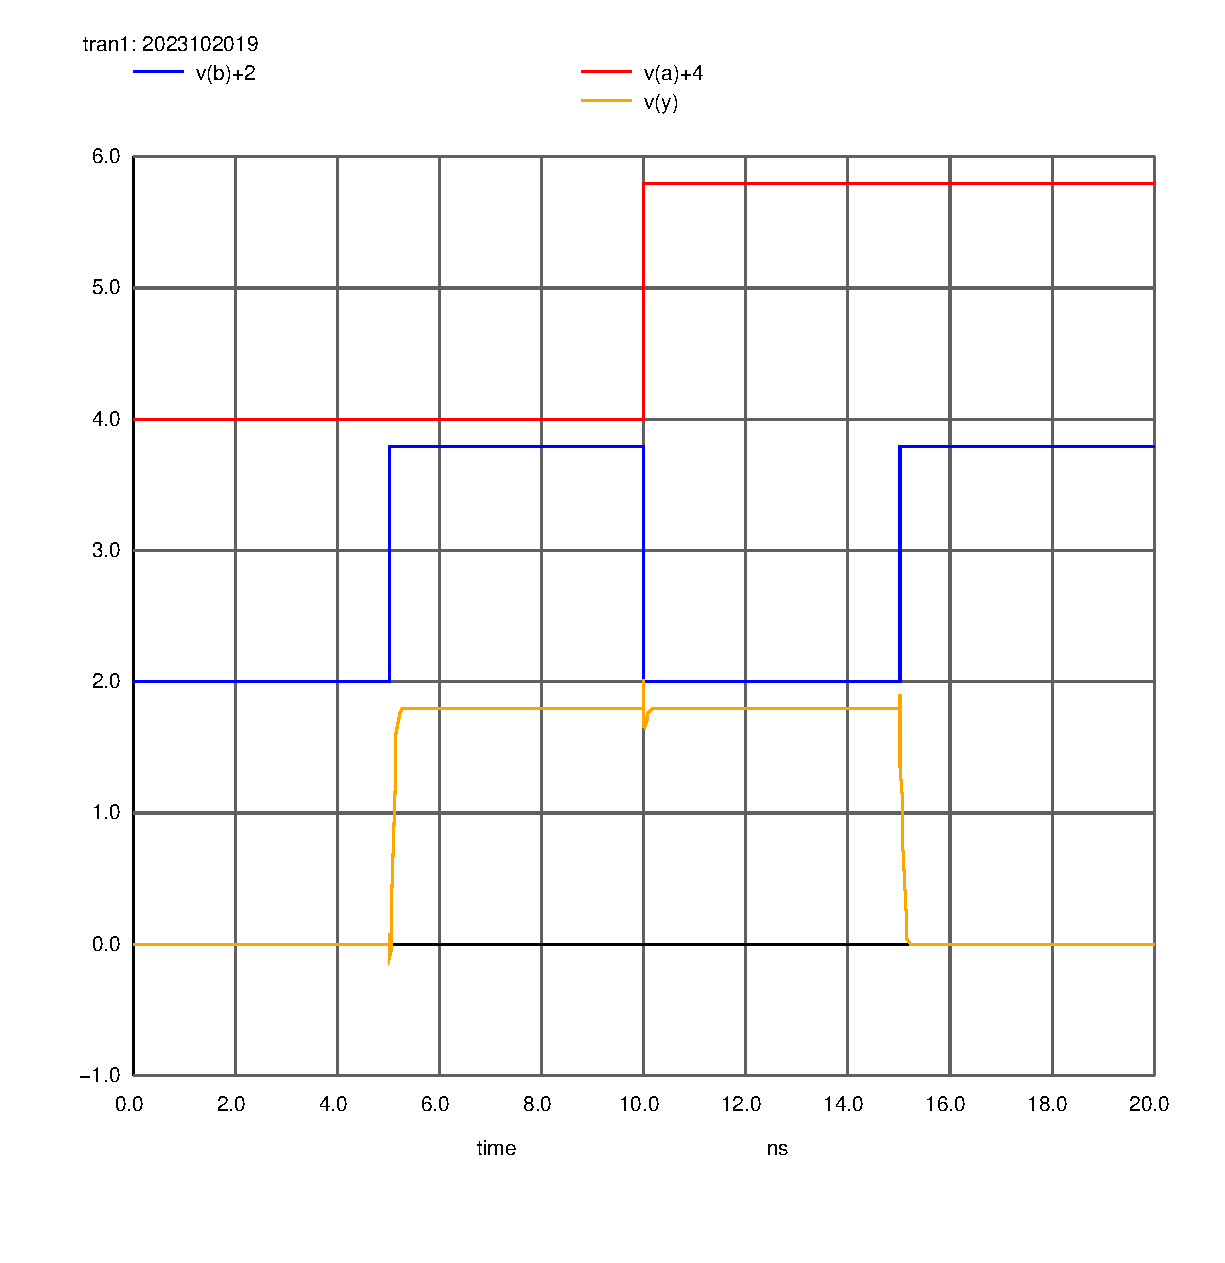
\includegraphics[width=0.48\textwidth]{images/xor_cmos_tran.eps}
    \caption{NGSPICE Plot of CMOS XOR Gate}
\end{figure}

\subsubsection{Complimentary Pass Transistor Implementation}

We use a CPTL XOR gate to reduce the number of transistors used.

\begin{figure}[H]
    \centering
    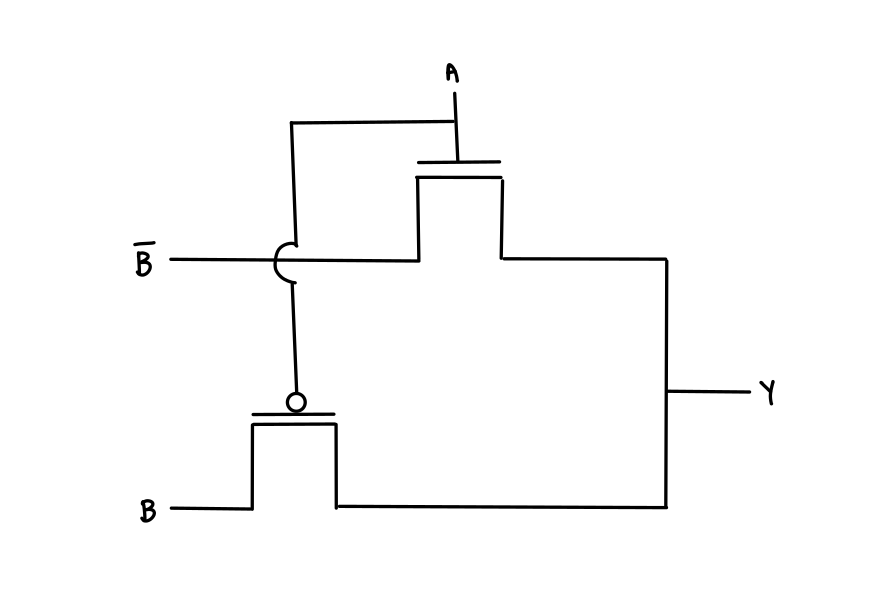
\includegraphics[width=0.48\textwidth]{images/xor_optimized_circuit_diagram.png}
    \caption{Circuit Diagram of CPTL XOR Gate}
\end{figure}

\begin{figure}[H]
    \centering
    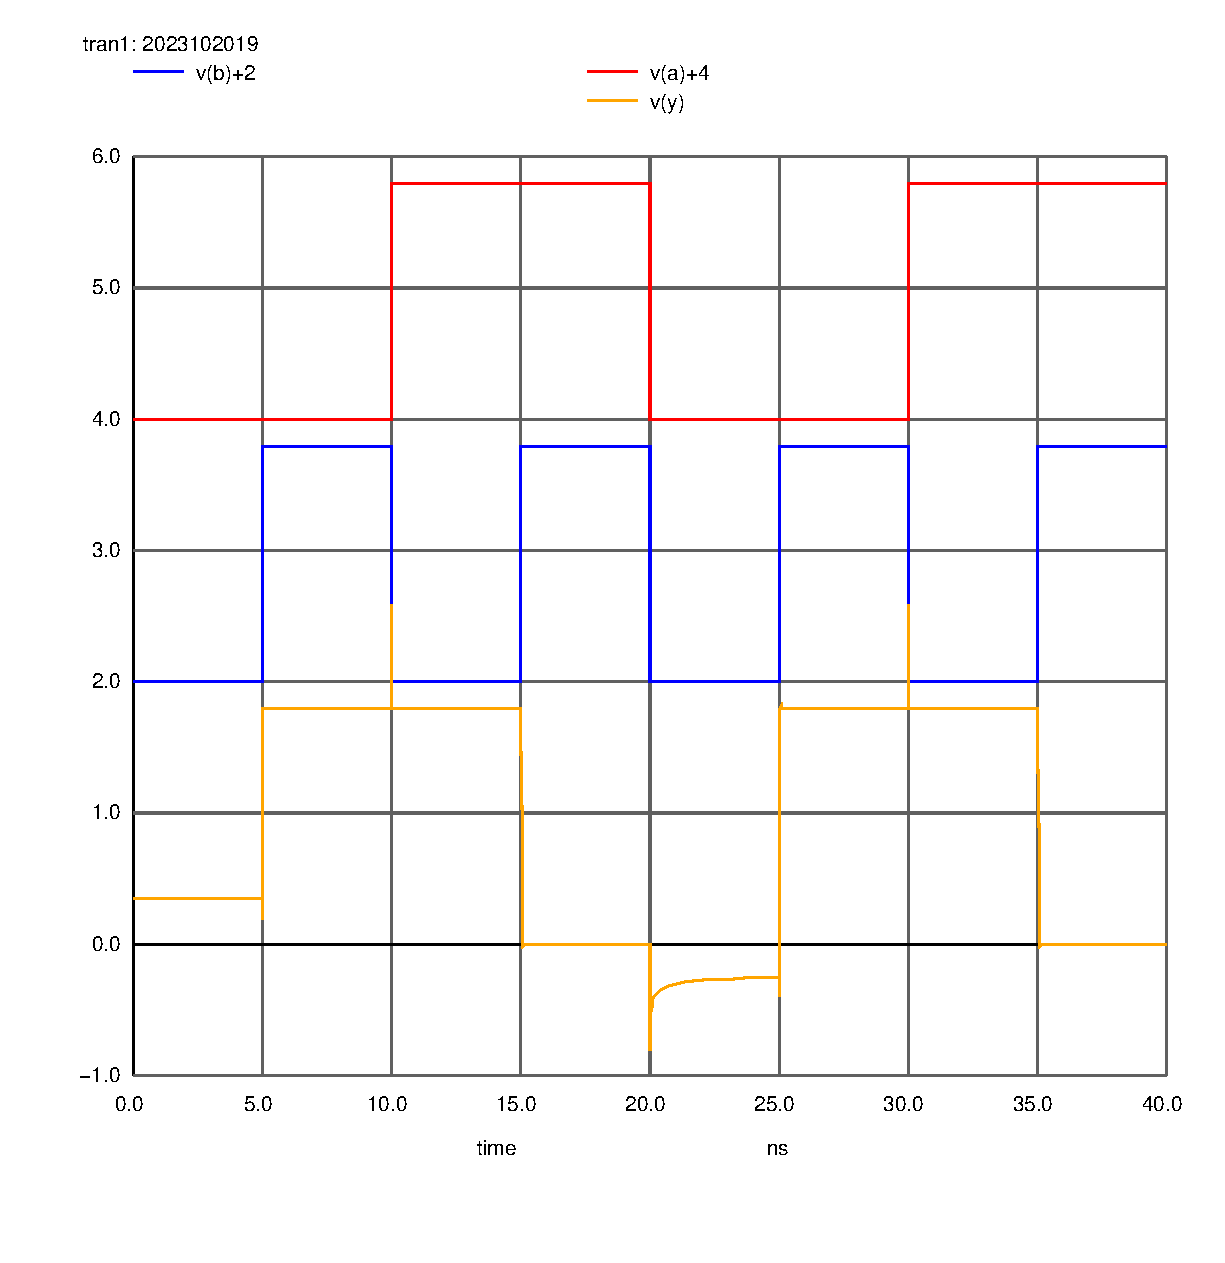
\includegraphics[width=0.48\textwidth]{images/xor_optimized_tran.eps}
    \caption{NGSPICE Plot of CPTL XOR Gate}
\end{figure}

Because of the nature of NMOS and PMOS and not being able to pass proper values, this does ruin the levels of the outputs, but from testing I have noticed that this does not affect the final result.

\subsection{Propagate/Generate Generator}

\subsubsection{CMOS Implementation}

Using the circuit diagram in \ref{fig:cla}, we can implement the Propagate/Generate Generator using the previously defined gates by importing them into our NGSPICE files. First, we test it using the CMOS Implementation of XOR.

\begin{figure}[H]
    \centering
    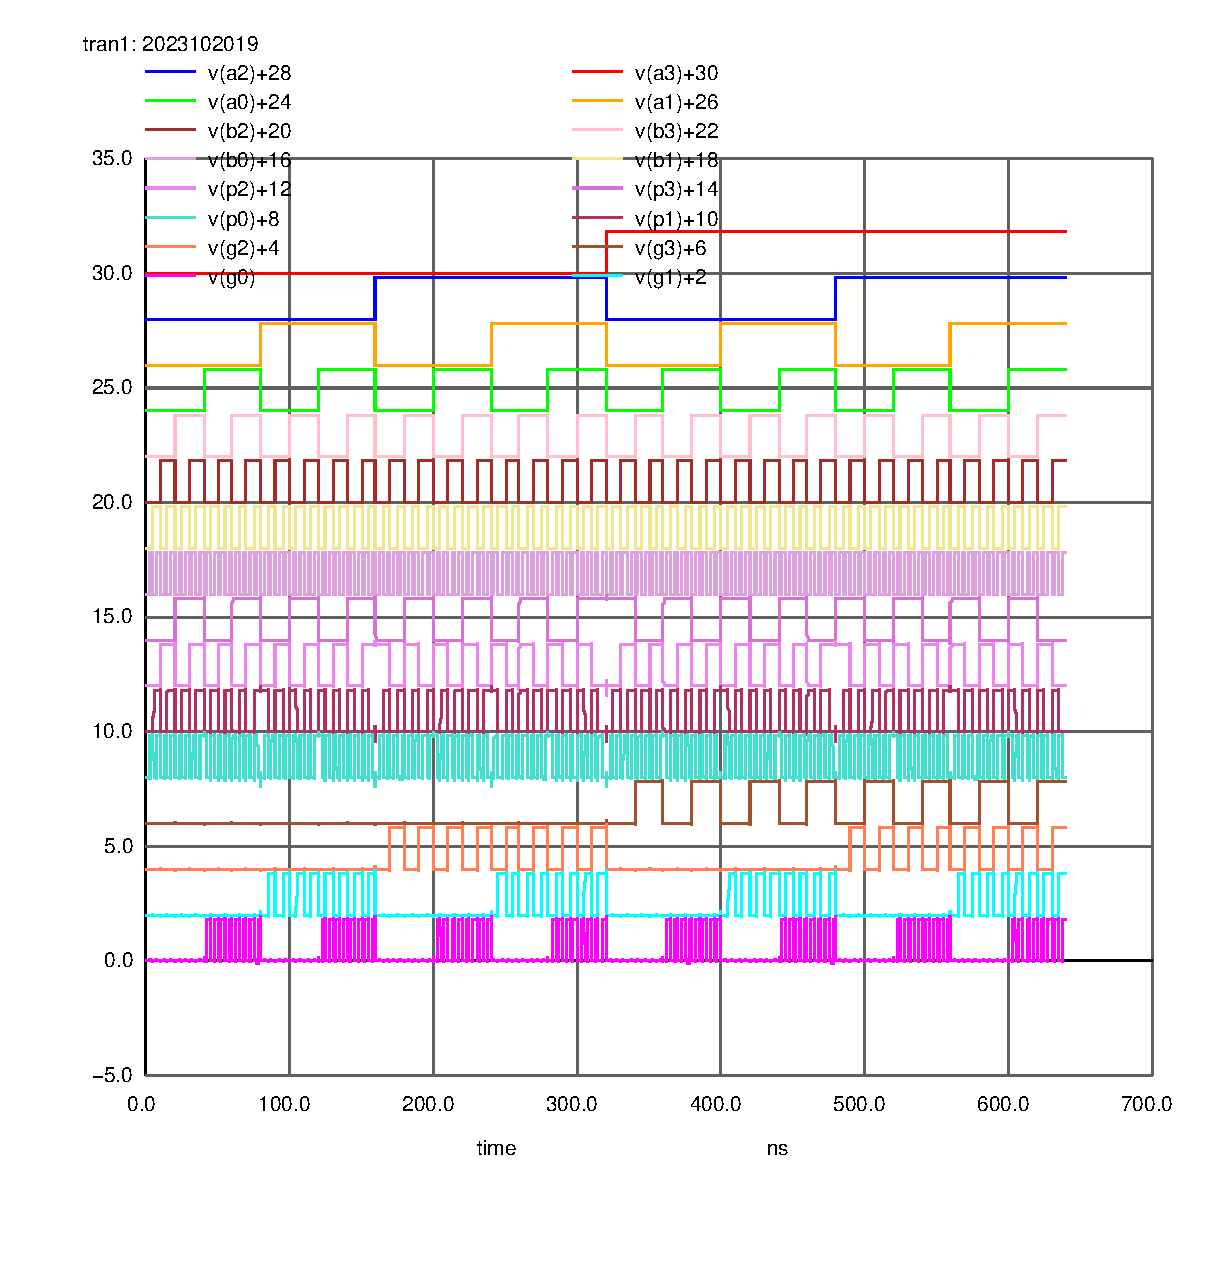
\includegraphics[width=0.48\textwidth]{images/pg_gen_cmos_tran.eps}
    \caption{NGSPICE Plot of CMOS Propagate/Generate Generator}
\end{figure}

\subsubsection{Complimentary Pass Transistor Implementation}

This is a test run using the CPTL XOR gate.

\begin{figure}[H]
    \centering
    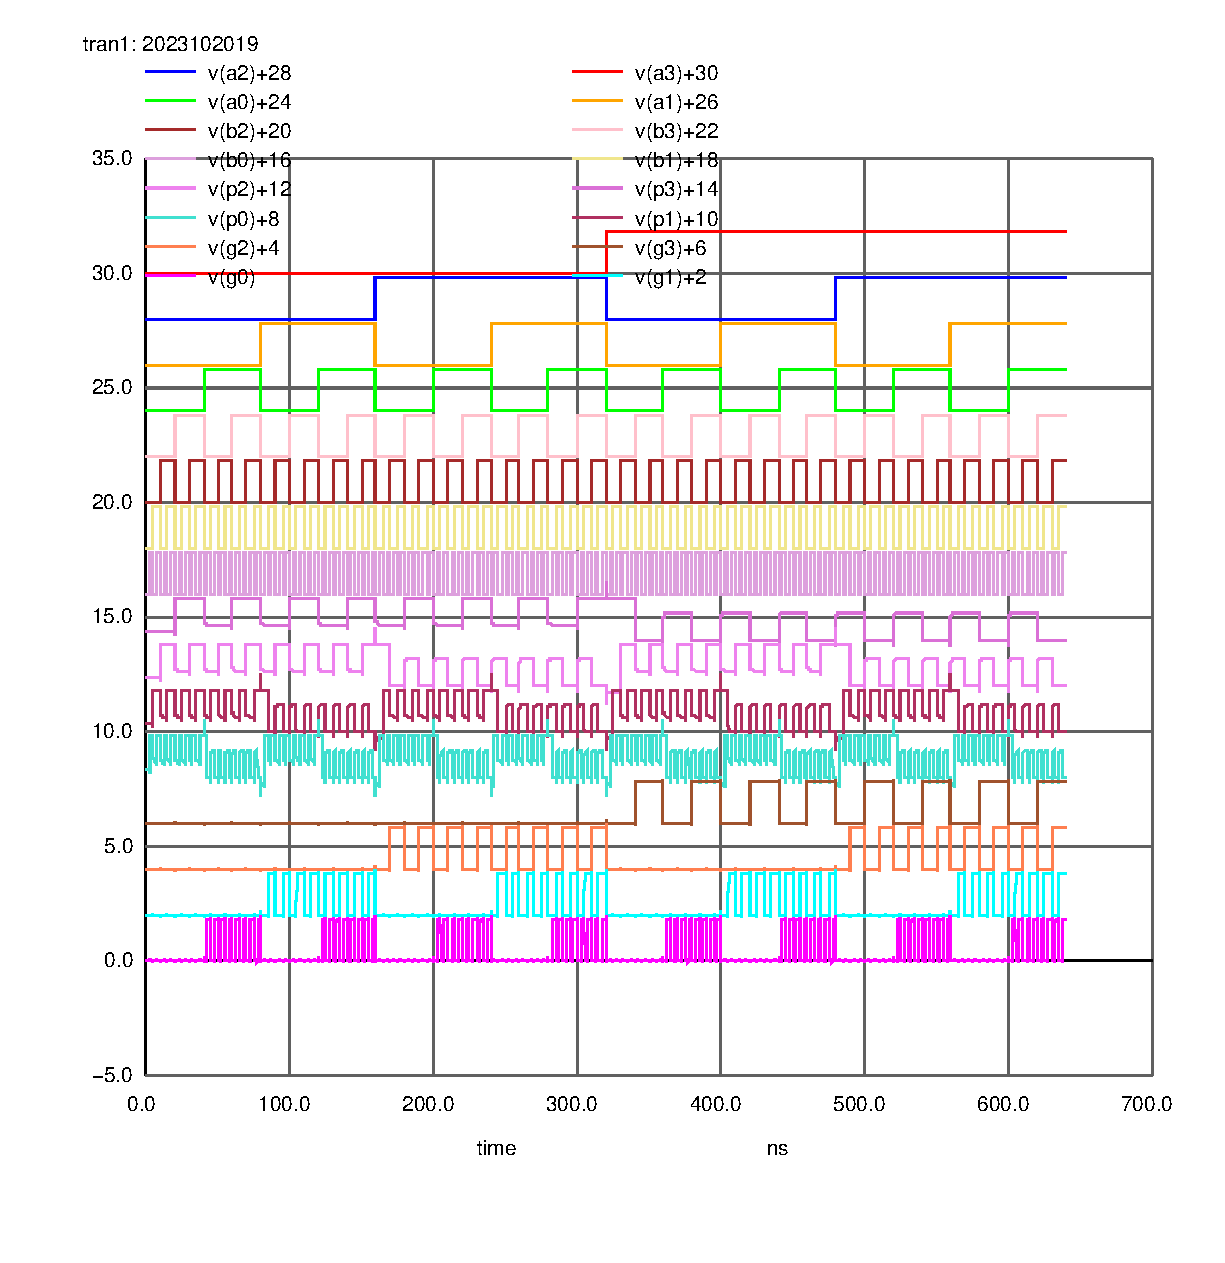
\includegraphics[width=0.48\textwidth]{images/pg_gen_optimized_tran.eps}
    \caption{NGSPICE Plot of CPTL Propagate/Generate Generator}
\end{figure}

We can already see massive issues in the levels of some of the outputs. This might seem concerning but it all gets fixed in the final circuit due to the nature of the D Flip Flop used.

\subsection{Carry Look Ahead Generator}

The Carry Look Ahead Generator is implemented only using CMOS gates.

\begin{figure}[H]
    \centering
    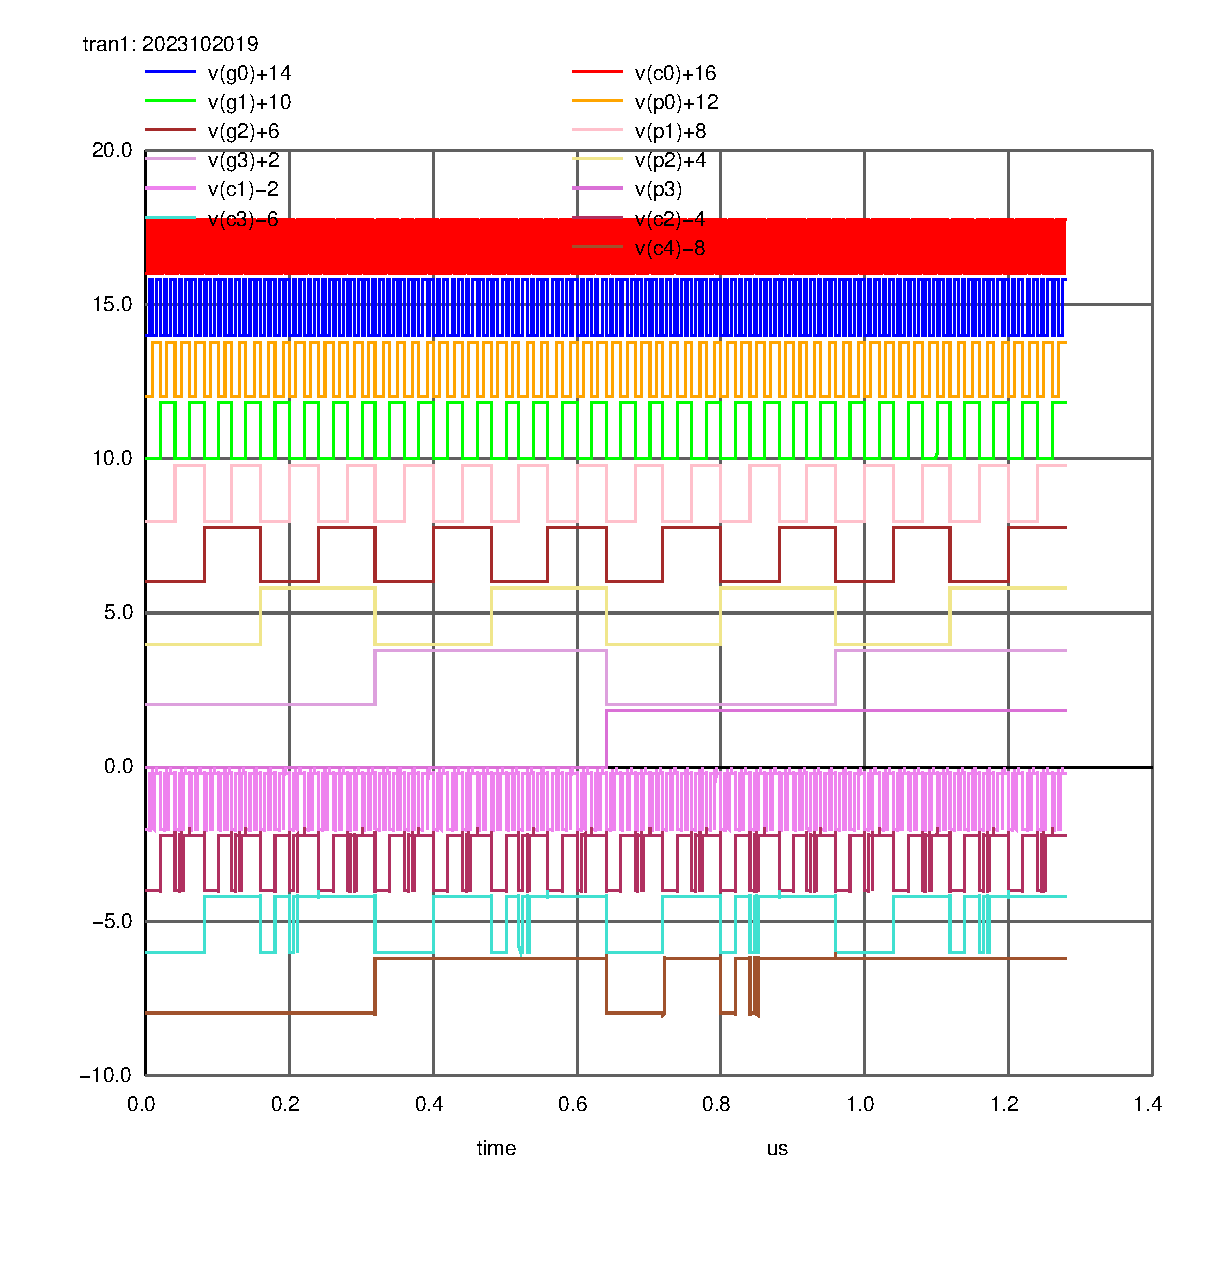
\includegraphics[width=0.48\textwidth]{images/cla_gen_cmos_tran.eps}
    \caption{NGSPICE Plot of CMOS Carry Look Ahead Generator}
\end{figure}

\subsection{Sum Generator}

\subsubsection{CMOS Implementation}

We similarly use the CMOS gates to implement the Sum Generator.

\begin{figure}[H]
    \centering
    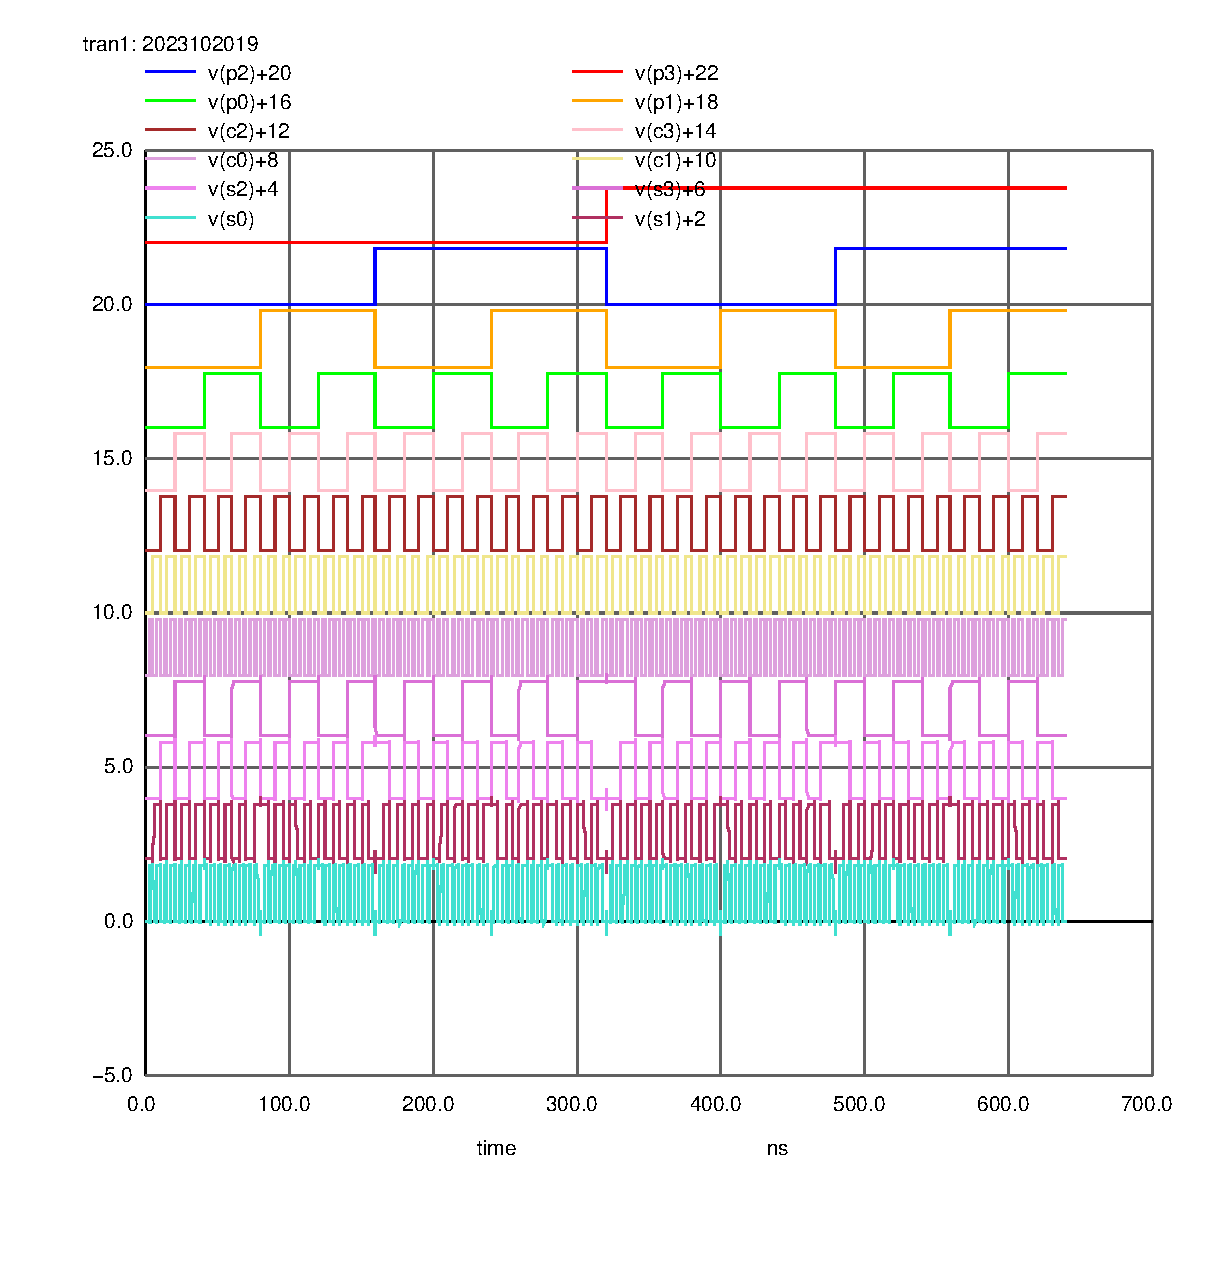
\includegraphics[width=0.48\textwidth]{images/sum_gen_cmos_tran.eps}
    \caption{NGSPICE Plot of CMOS Sum Generator}
\end{figure}

\subsubsection{Complimentary Pass Transistor Implementation}

We can see that the levels of the outputs are not correct in this circuit either, due to the nature of the CPTL XOR gate.

\begin{figure}[H]
    \centering
    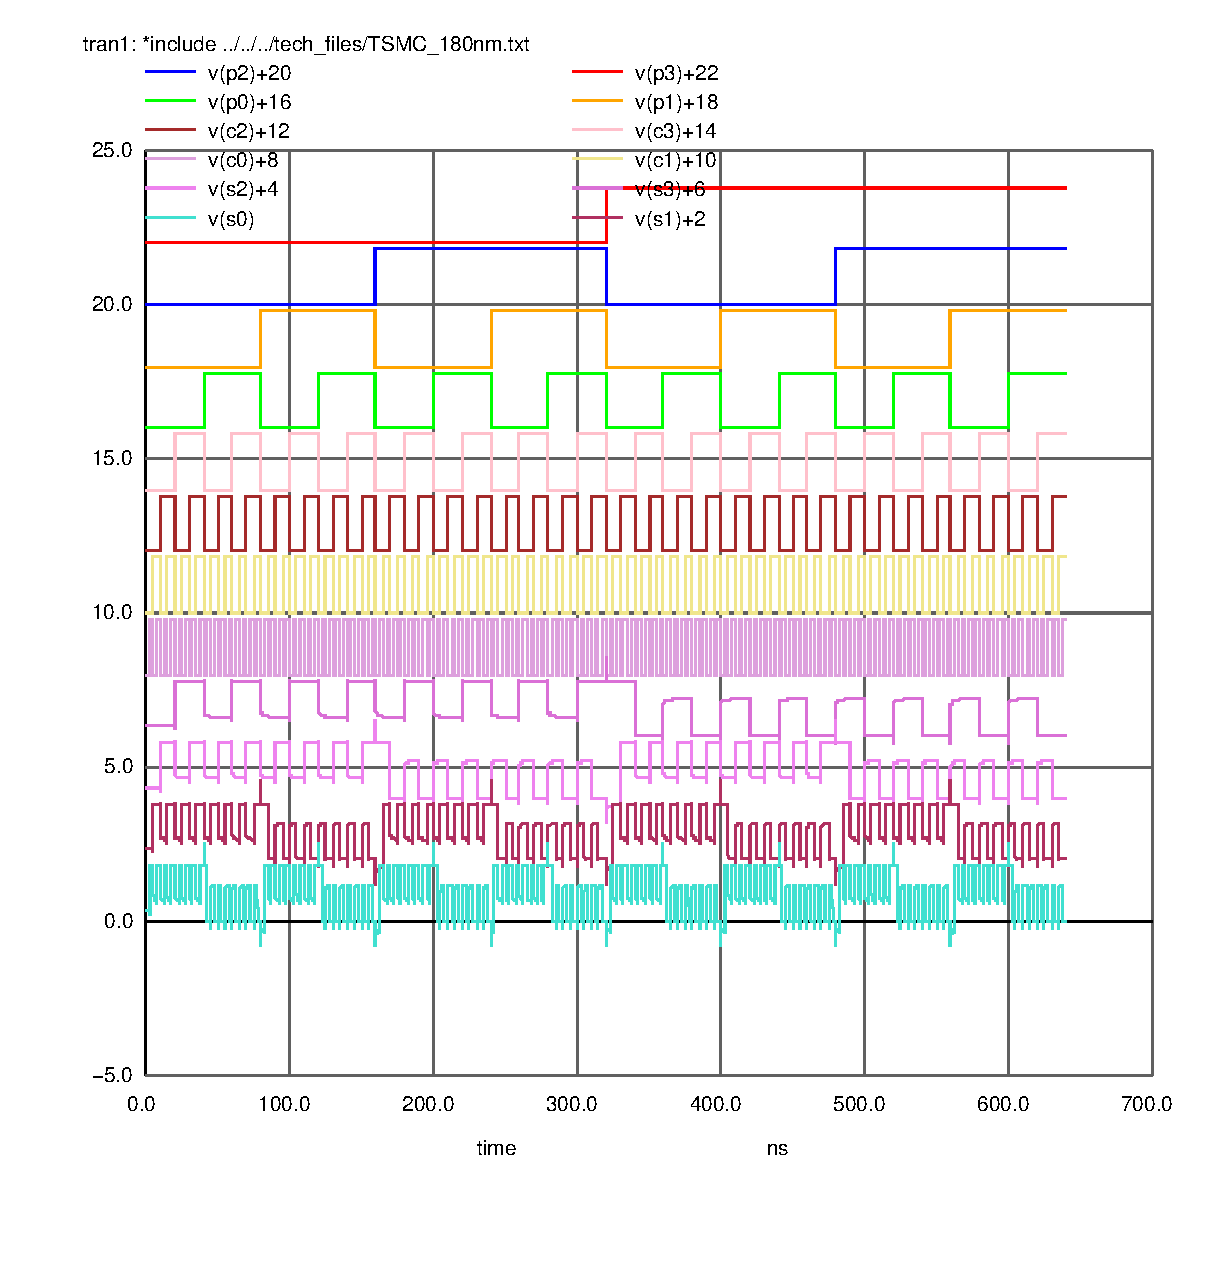
\includegraphics[width=0.48\textwidth]{images/sum_gen_optimized_tran.eps}
    \caption{NGSPICE Plot of CPTL Sum Generator}
\end{figure}

\subsection{D Flop Flop}

\subsubsection{CMOS Implementation}

We make the D Flip Flop using the CMOS gates, but as we noticed before, this is not the best way to implement it.

\begin{figure}[H]
    \centering
    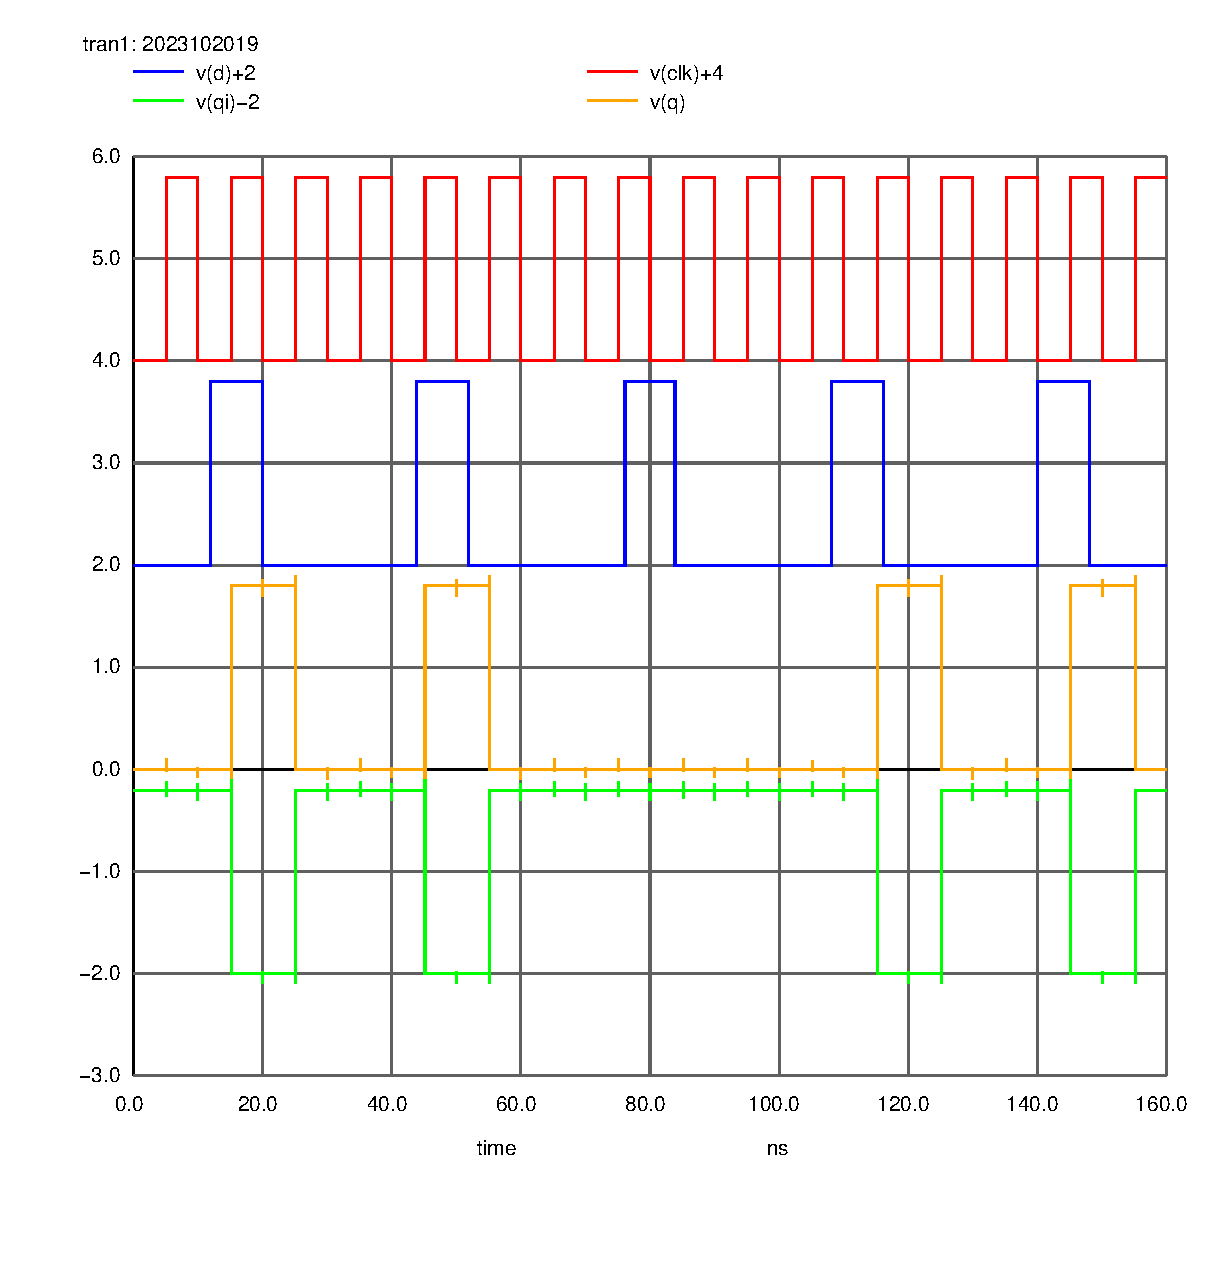
\includegraphics[width=0.48\textwidth]{images/d_ff_cmos_tran.eps}
    \caption{NGSPICE Plot of CMOS D Flip FLop}
\end{figure}

\subsubsection{Optimized Implementation}

Making the D Flip Flop using our optimized circuit works as well:

\begin{figure}[H]
    \centering
    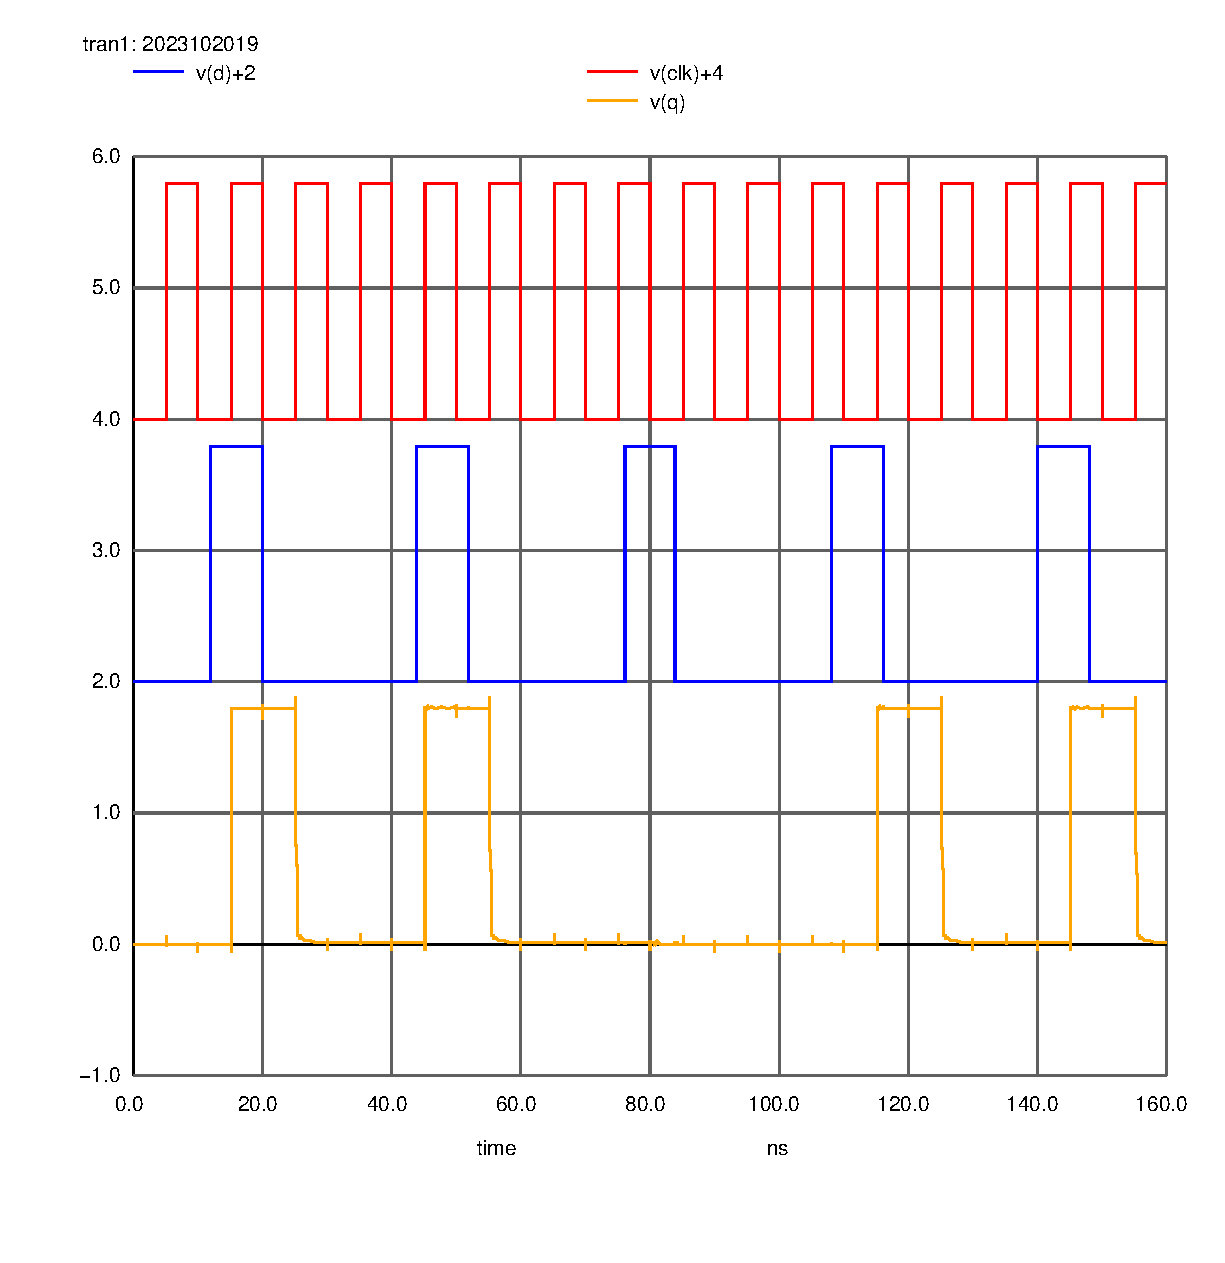
\includegraphics[width=0.48\textwidth]{images/d_ff_optimized_tran.eps}
    \caption{NGSPICE Plot of Optimized D Flip Flop}
\end{figure}

We can find the characteristics of the D Flip Flop as follows:

\begin{enumerate}
    \item $t_{\text{cq}}$ is the time taken for the output Q to change after the rising clock edge.
    \item $t_{\text{su}}$ is the setup time, the time before the rising clock edge that the input D must be stable. We calculate this based on the rise/fall time of the mosfet that passes the input D, and the propagation delay of the inverter that stores the value in the flip flop.
    \item $t_{\text{h}}$ is the hold time, the time after the rising clock edge that the input D must be stable. We calculate this based on the rise/fall time of the mosfet that passes the input D, and the propagation delay of the inverter that returns the output of the flip flop.
\end{enumerate}

We get these values using: 

\begin{align}
    t_{\text{cq}} &= t_q - t_{\text{clk}} \quad \text{(at } 0.5 \cdot \text{SUPPLY)} \\
    t_{\text{su}} &= t_{\text{rise}_{M1}} + t_{\text{prop}_{\text{inv1}}} \\
    t_{\text{h}} &= t_{\text{rise}_{M2}} + t_{\text{prop}_{\text{inv2}}}
\end{align}

\begin{verbatim}
    t_cq                =  5.24757e-11ns
    t_su                =  3.80793e-10ns
    t_h                 =  2.67745e-10ns
\end{verbatim}

\subsection{Full Circuit}

\begin{figure}[H]
    \centering
    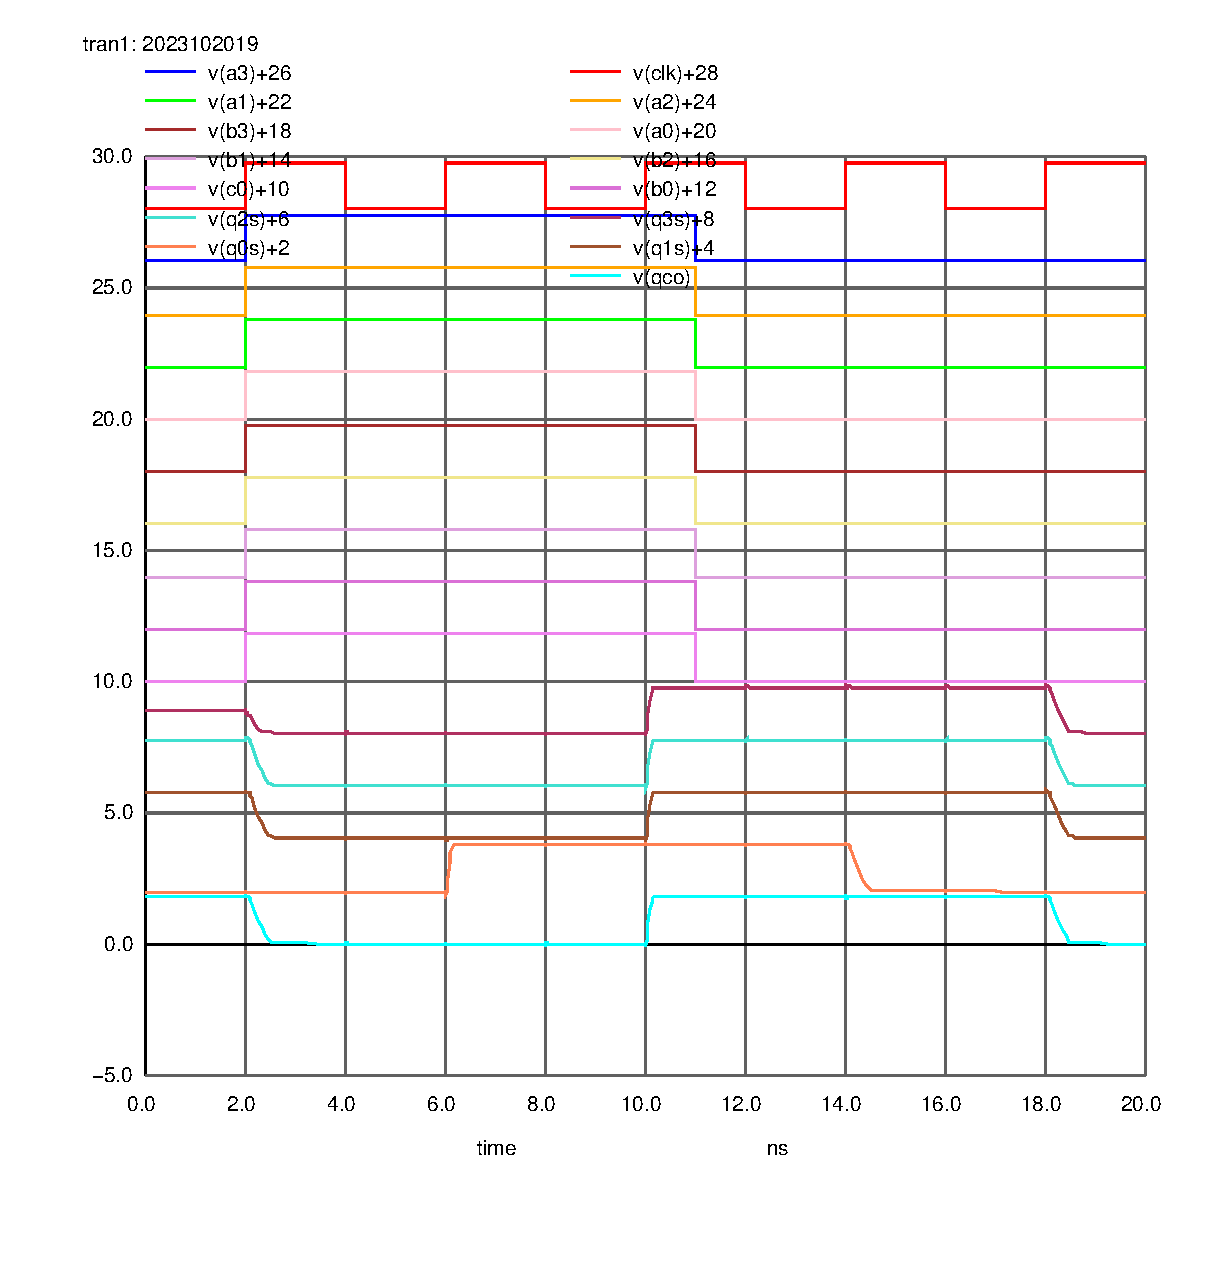
\includegraphics[width=0.48\textwidth]{images/full_optimized_tran.eps}
    \caption{NGSPICE Plot of Optimized Circuit}
\end{figure}

\section{MAGIC Layout}
For layout, we use the free tool MAGIC. All subcircuits are laid out separately and then combined to form the full circuit. Before layout, we draw stick diagrams to have a rough idea of where to place what.

\begin{figure*}[t]
    \centering
    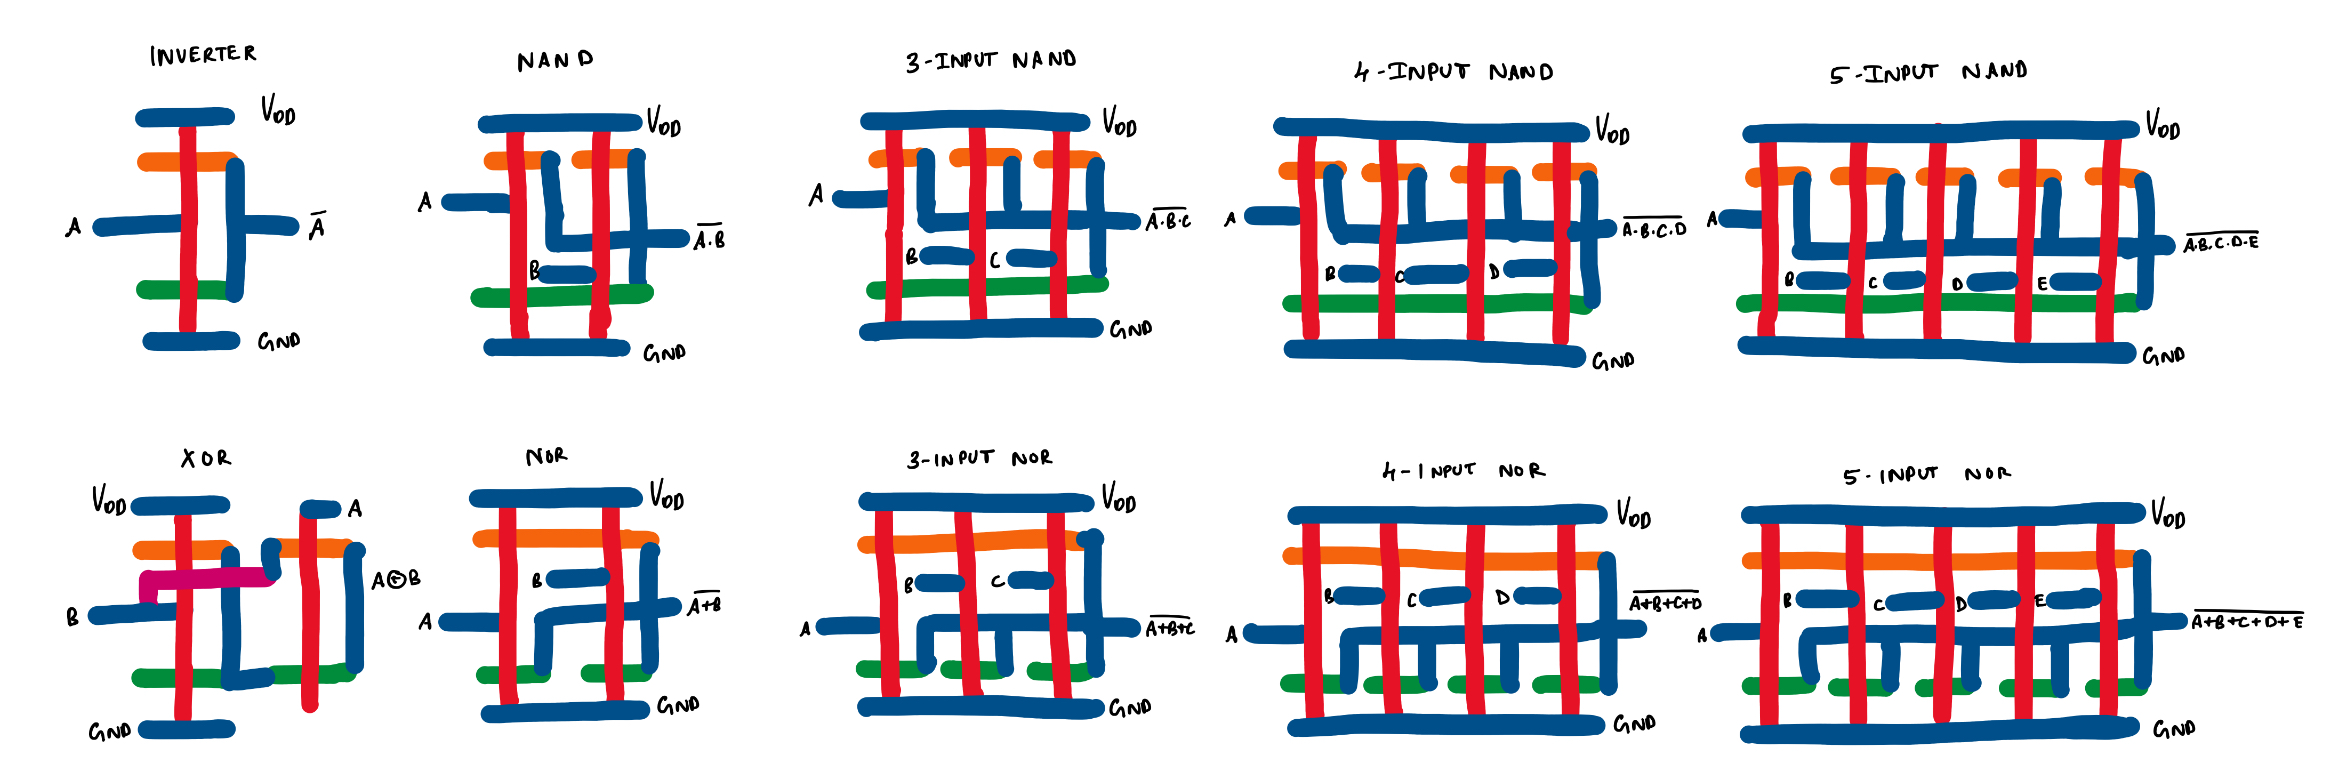
\includegraphics[width=0.8\textwidth]{images/stick_diagrams.png}
    \caption{Stick Diagrams}
\end{figure*}

\subsection{Inverter}

\begin{figure}[H]
    \centering
    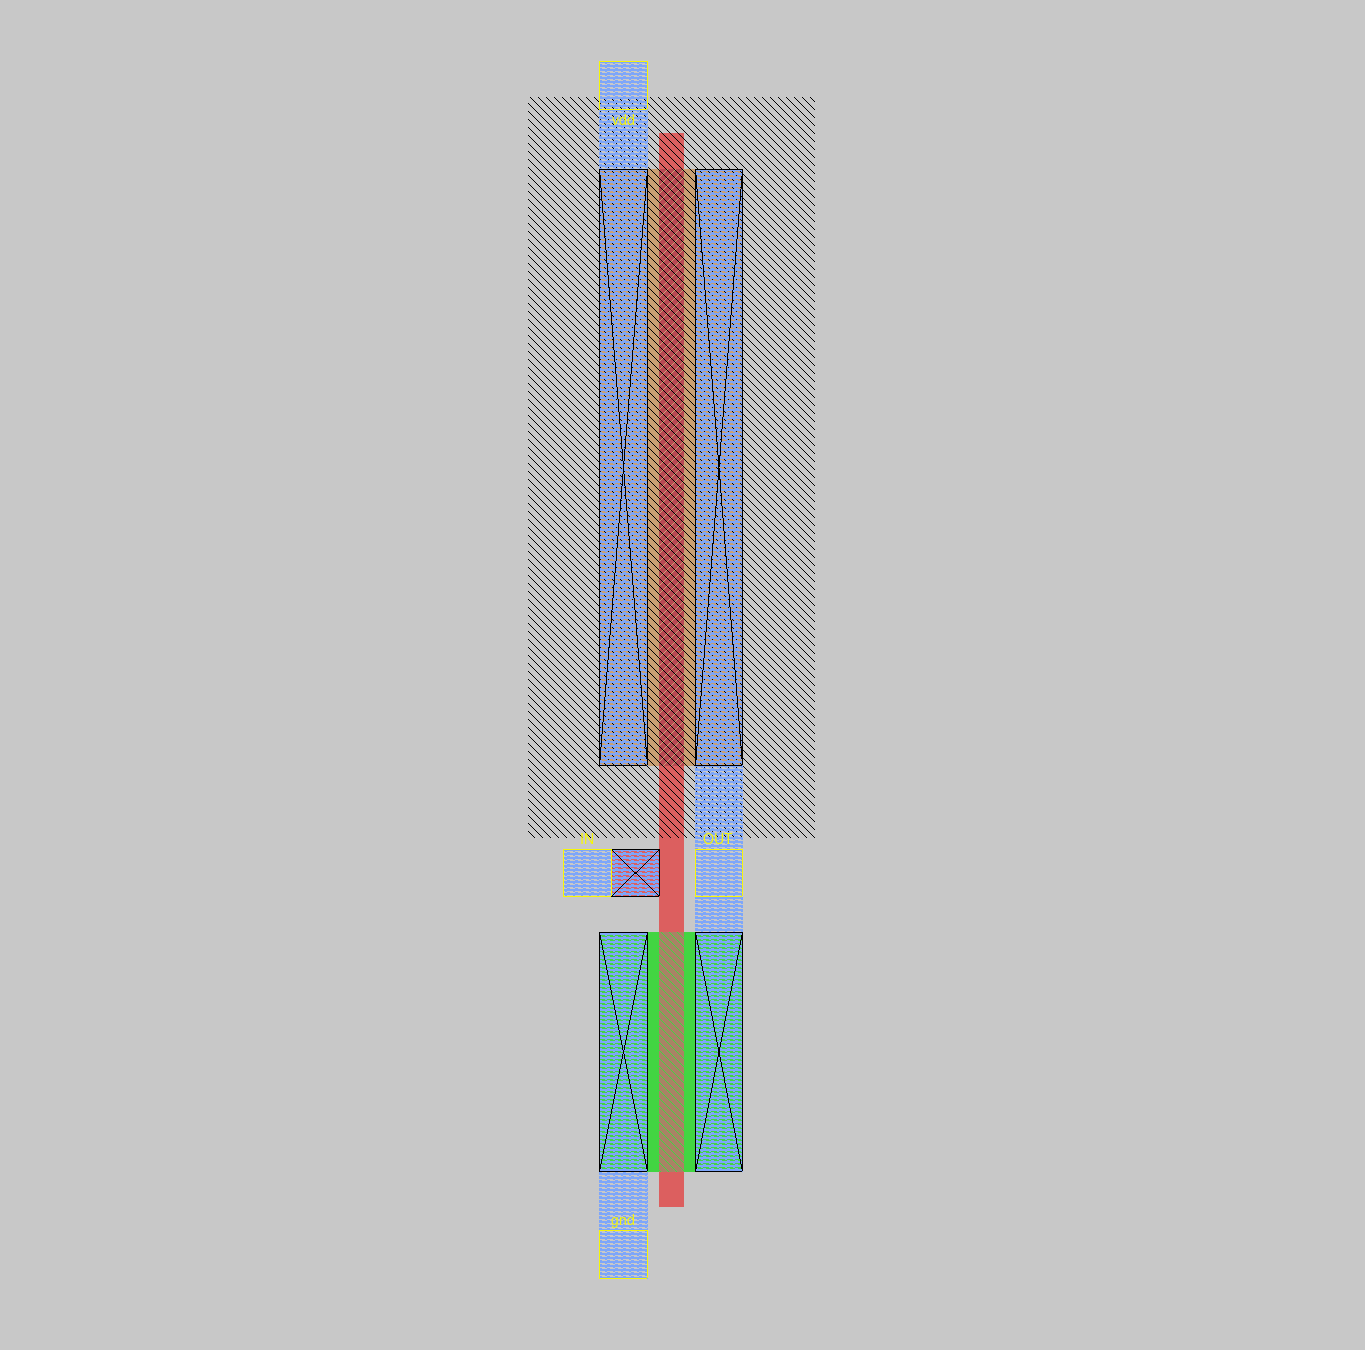
\includegraphics[width=0.48\textwidth]{images/inv_cmos_layout.png}
    \caption{MAGIC Layout of CMOS Inverter}
\end{figure}

\subsection{NAND Gate}

\begin{figure}[H]
    \centering
    \begin{tabular}{cc}
        \begin{subfigure}{0.44\linewidth}
            \centering
            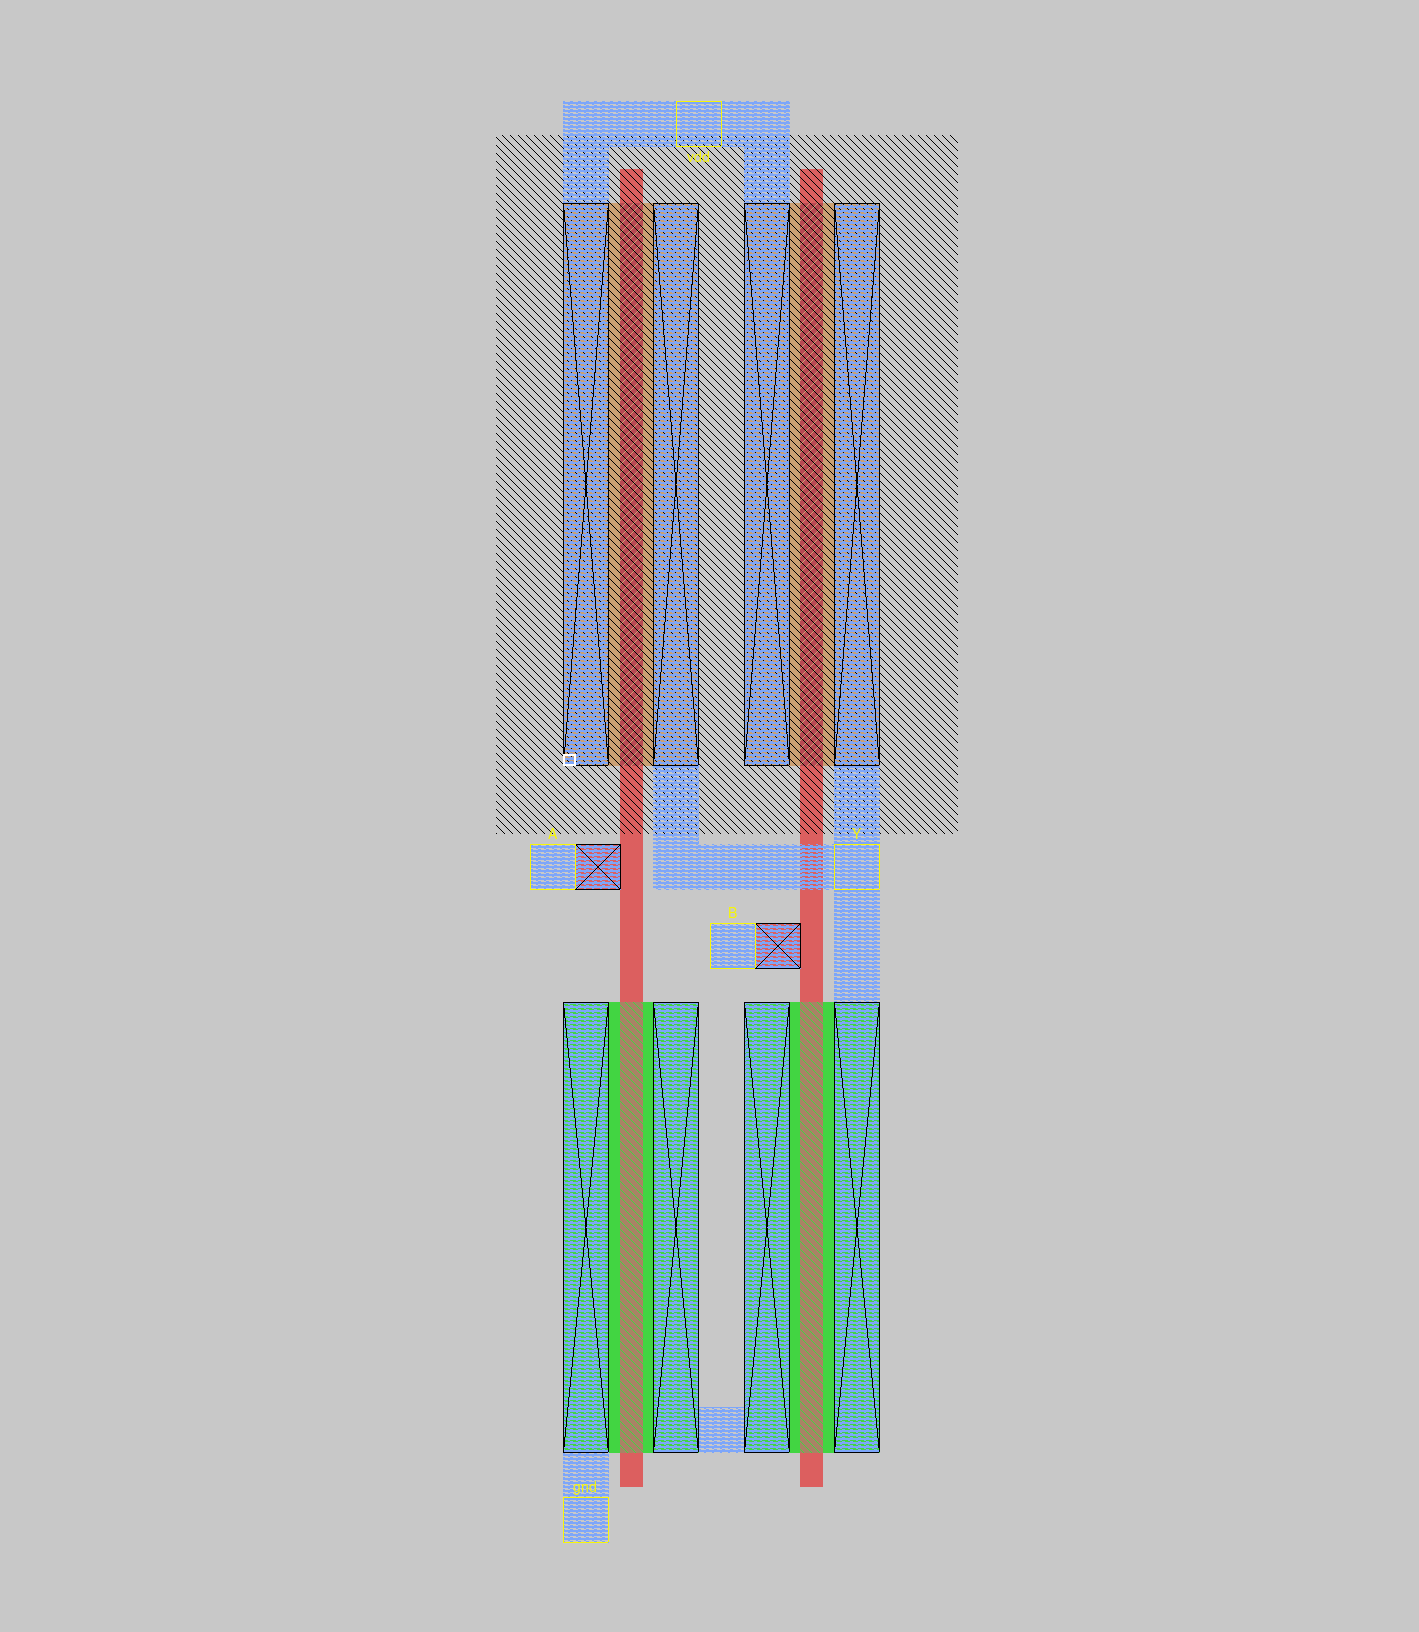
\includegraphics[width=\textwidth]{images/nand_cmos_layout.png}
            \caption{2 Input NAND}
        \end{subfigure} &
        \begin{subfigure}{0.44\linewidth}
            \centering
            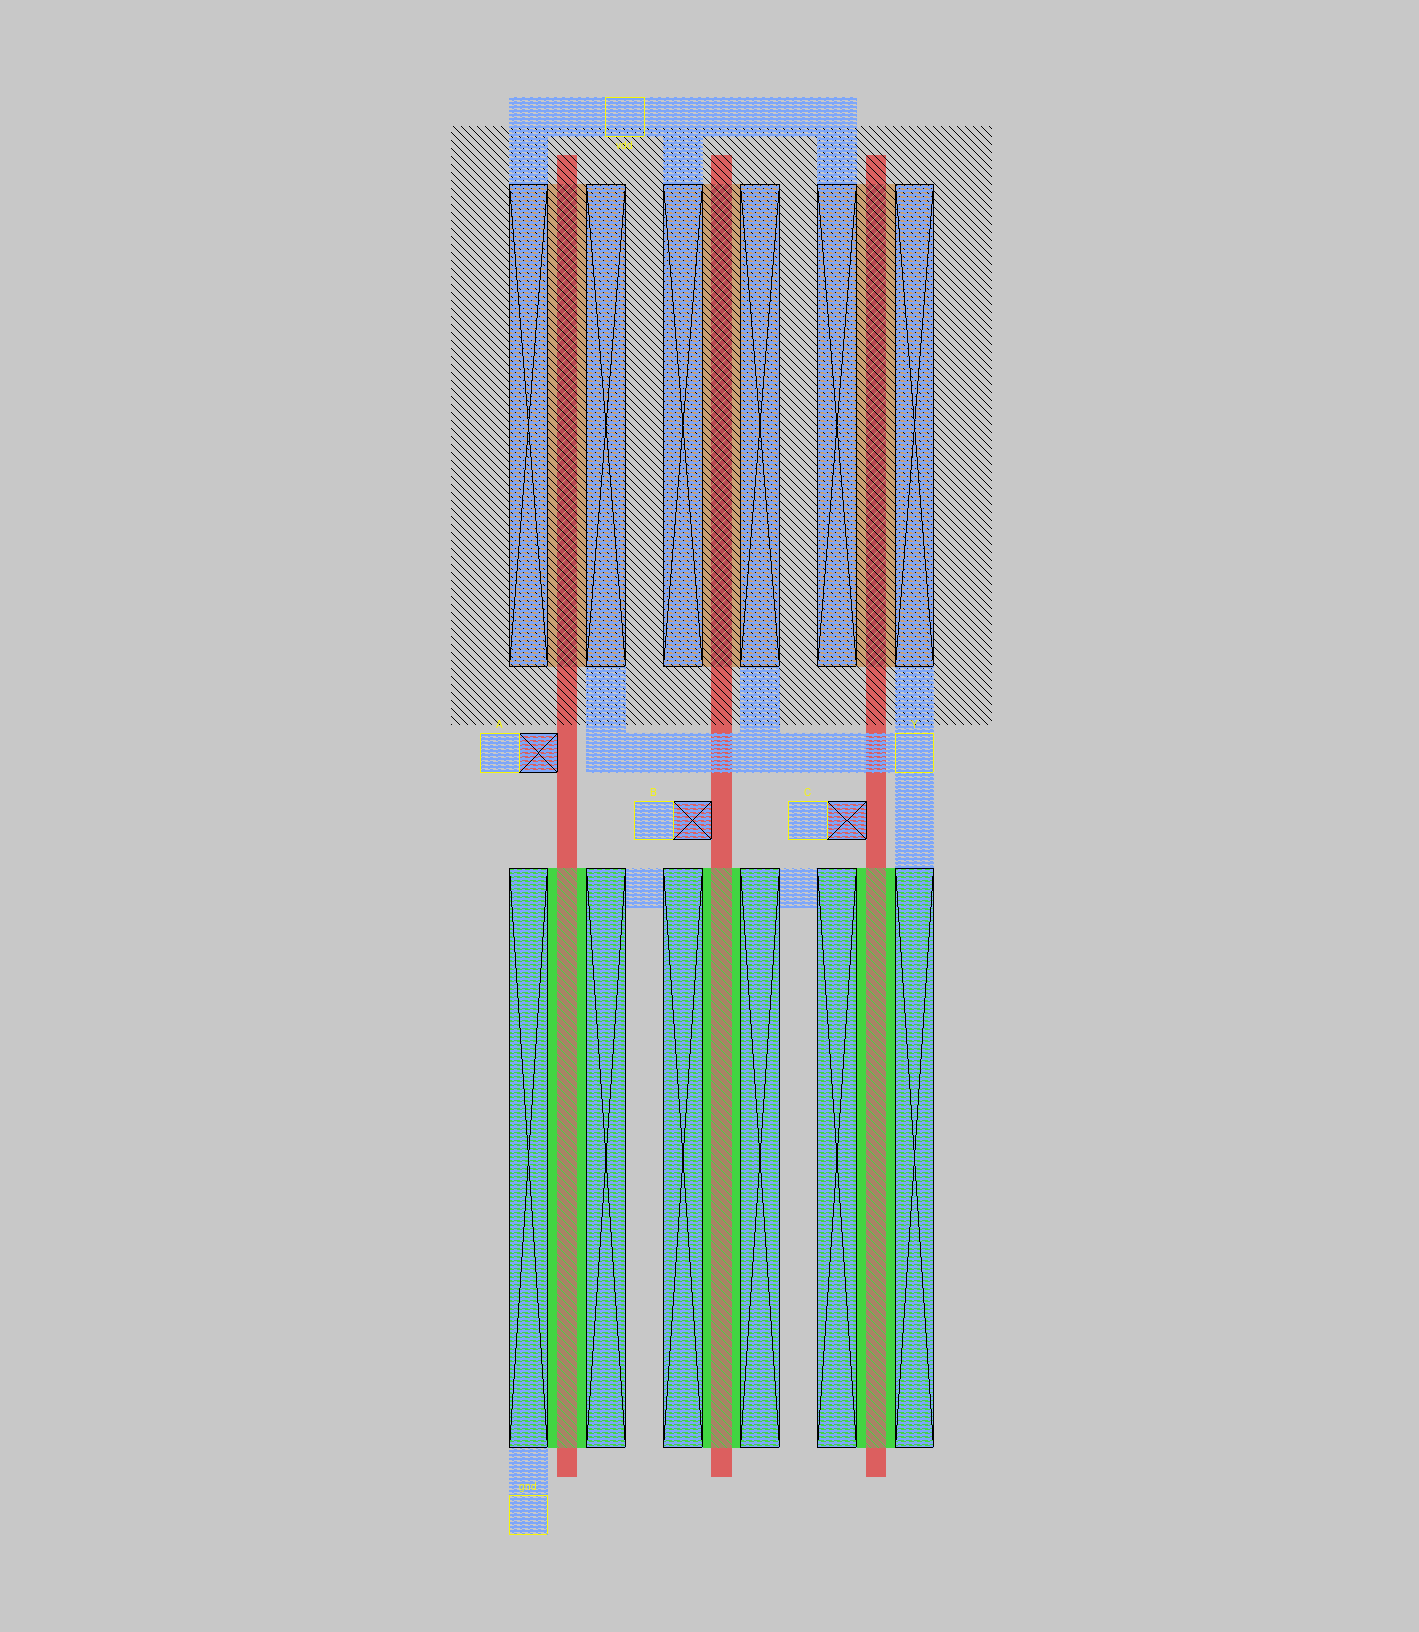
\includegraphics[width=\textwidth]{images/nand_3_cmos_layout.png}
            \caption{3 Input NAND}
        \end{subfigure} \\
        \begin{subfigure}{0.44\linewidth}
            \centering
            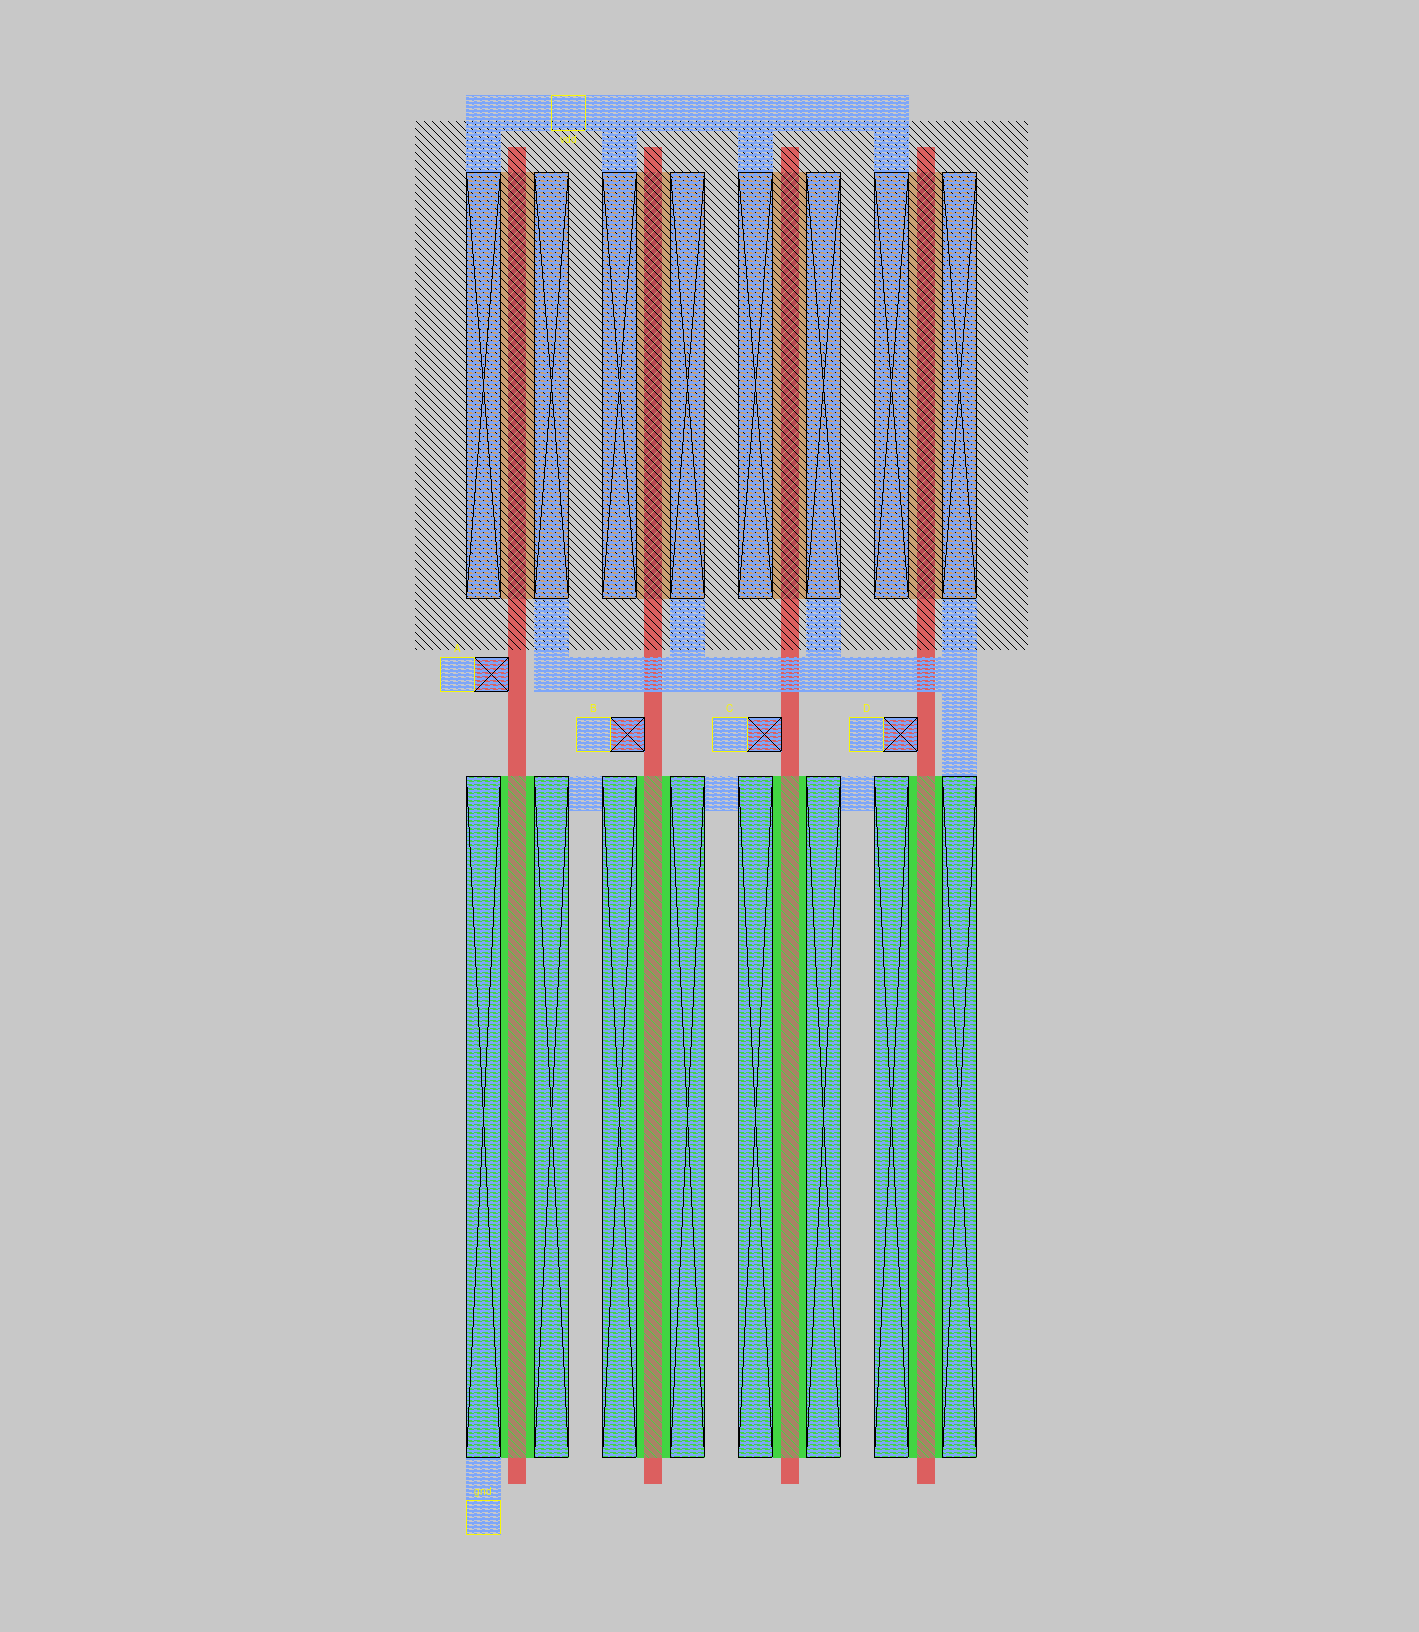
\includegraphics[width=\textwidth]{images/nand_4_cmos_layout.png}
            \caption{4 Input NAND}
        \end{subfigure} &
        \begin{subfigure}{0.44\linewidth}
            \centering
            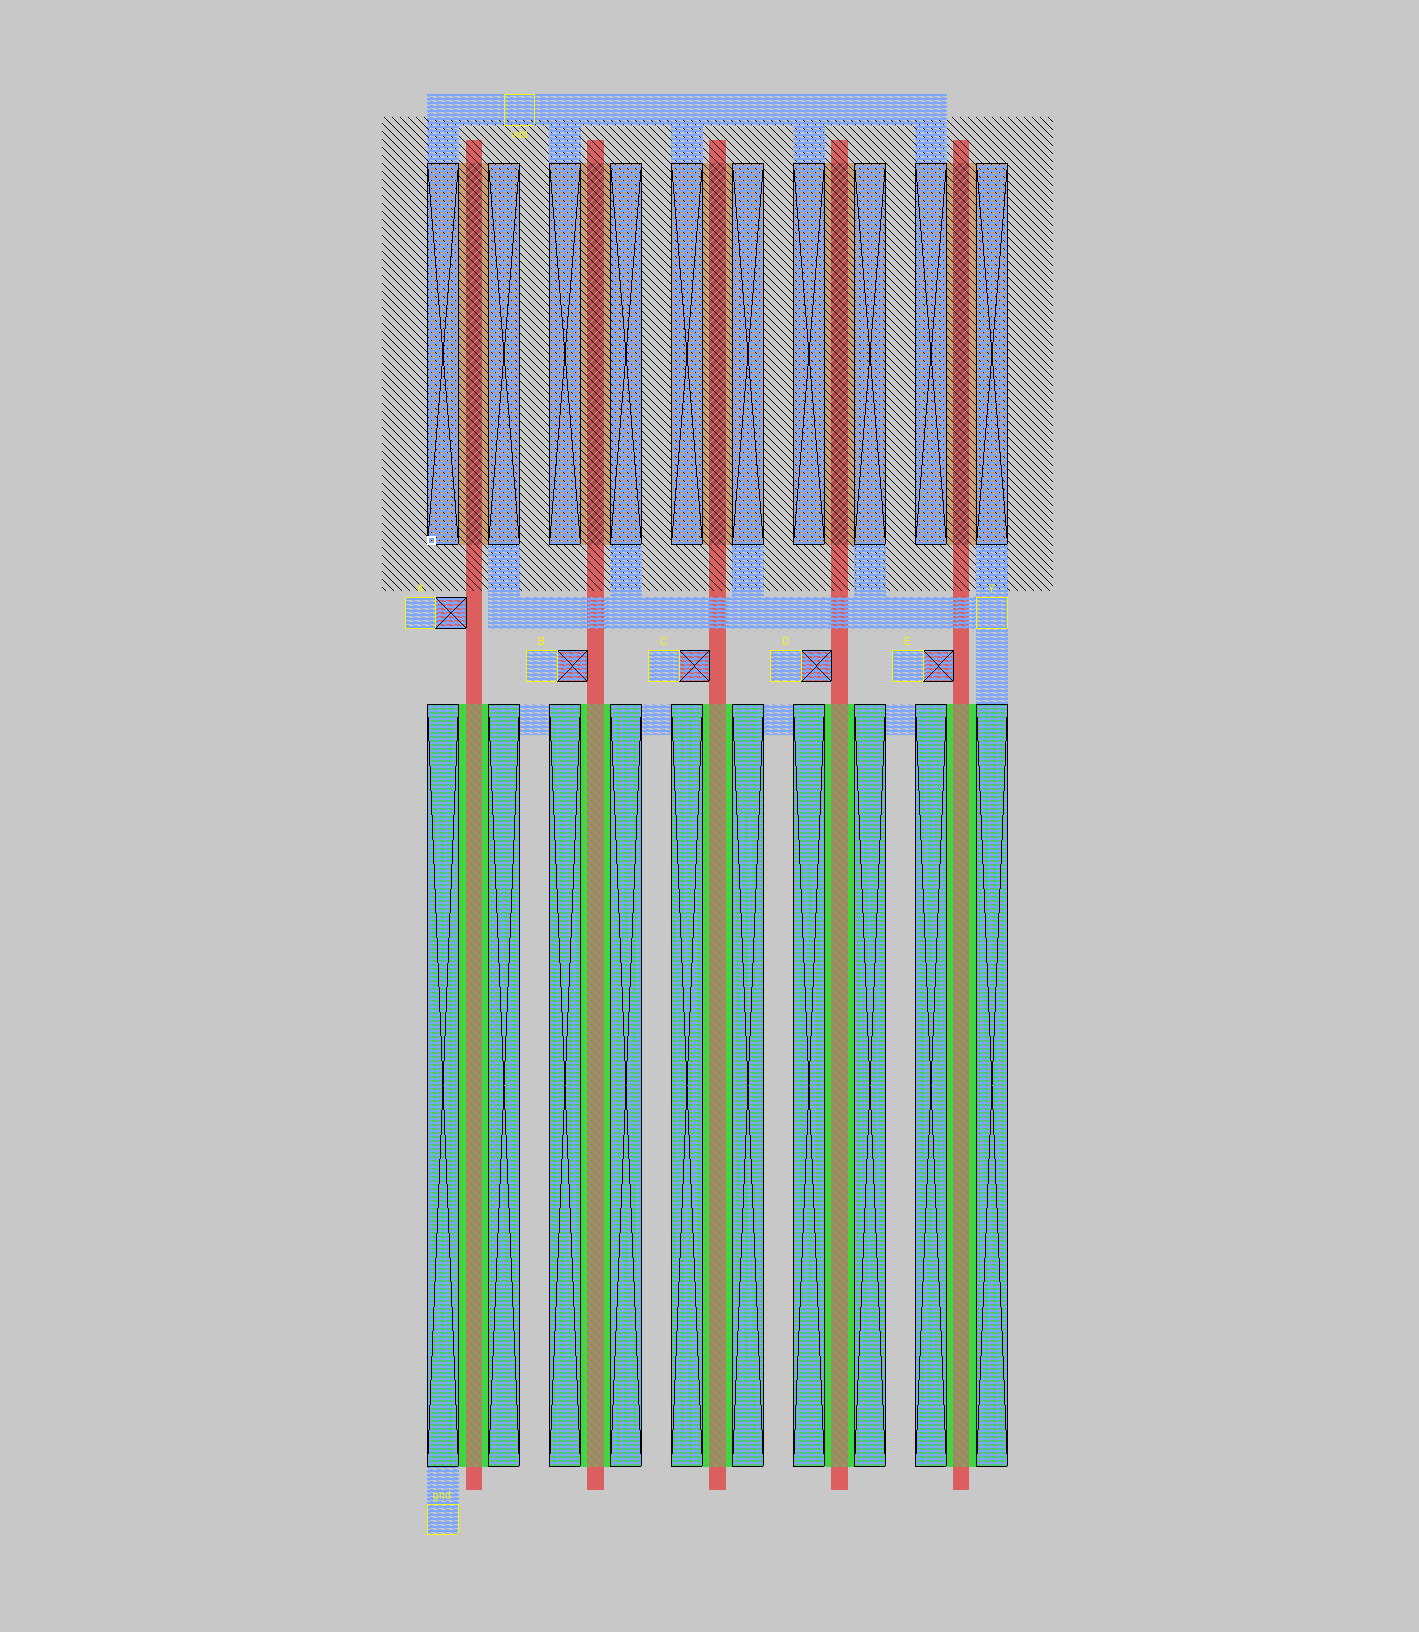
\includegraphics[width=\textwidth]{images/nand_5_cmos_layout.png}
            \caption{5 Input NAND}
        \end{subfigure}
    \end{tabular}
    \caption{MAGIC Layout of NAND Gates}
\end{figure}

\subsection{NOR Gate}

\begin{figure}[H]
    \centering
    \begin{tabular}{cc}
        \begin{subfigure}{0.44\linewidth}
            \centering
            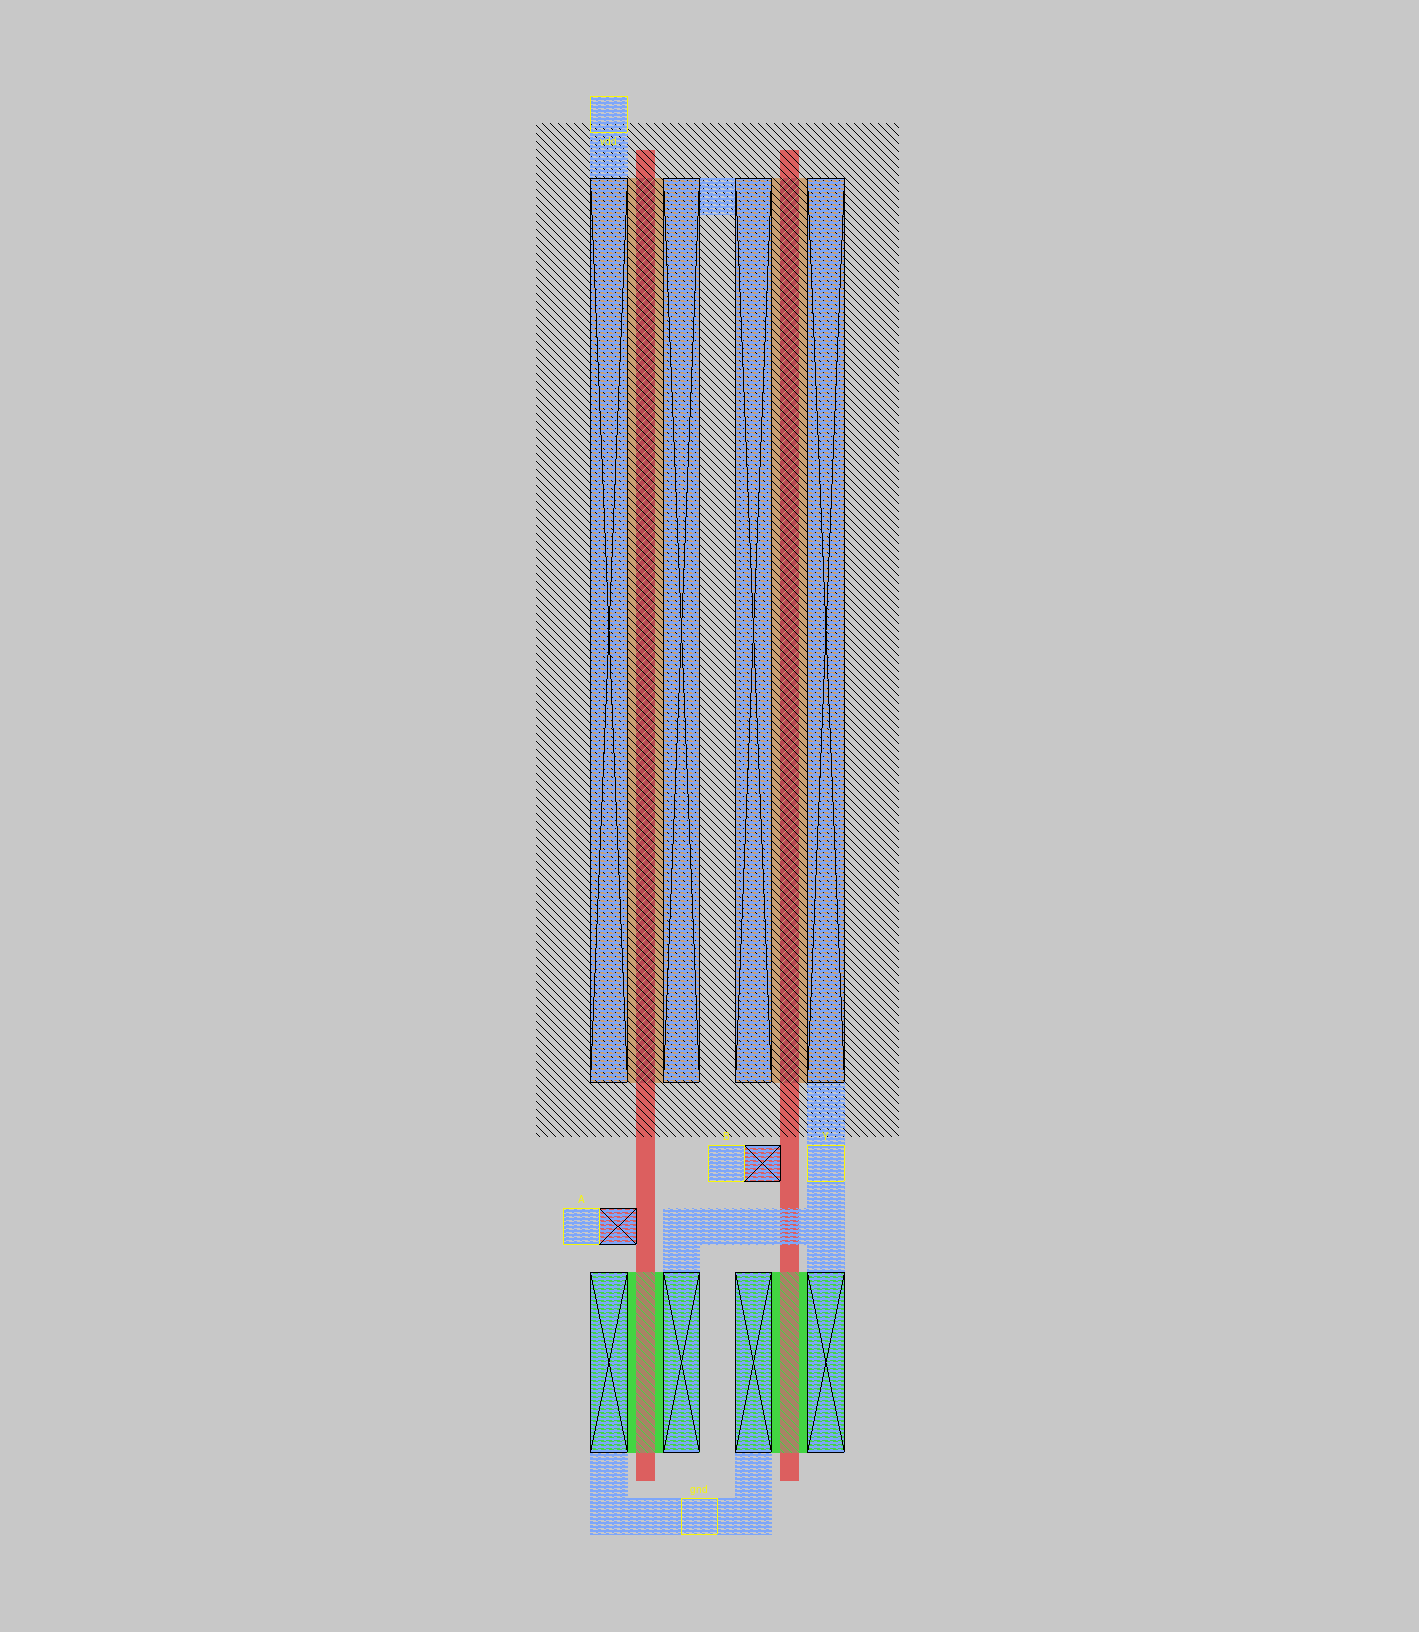
\includegraphics[width=\textwidth]{images/nor_cmos_layout.png}
            \caption{2 Input NOR}
        \end{subfigure} &
        \begin{subfigure}{0.44\linewidth}
            \centering
            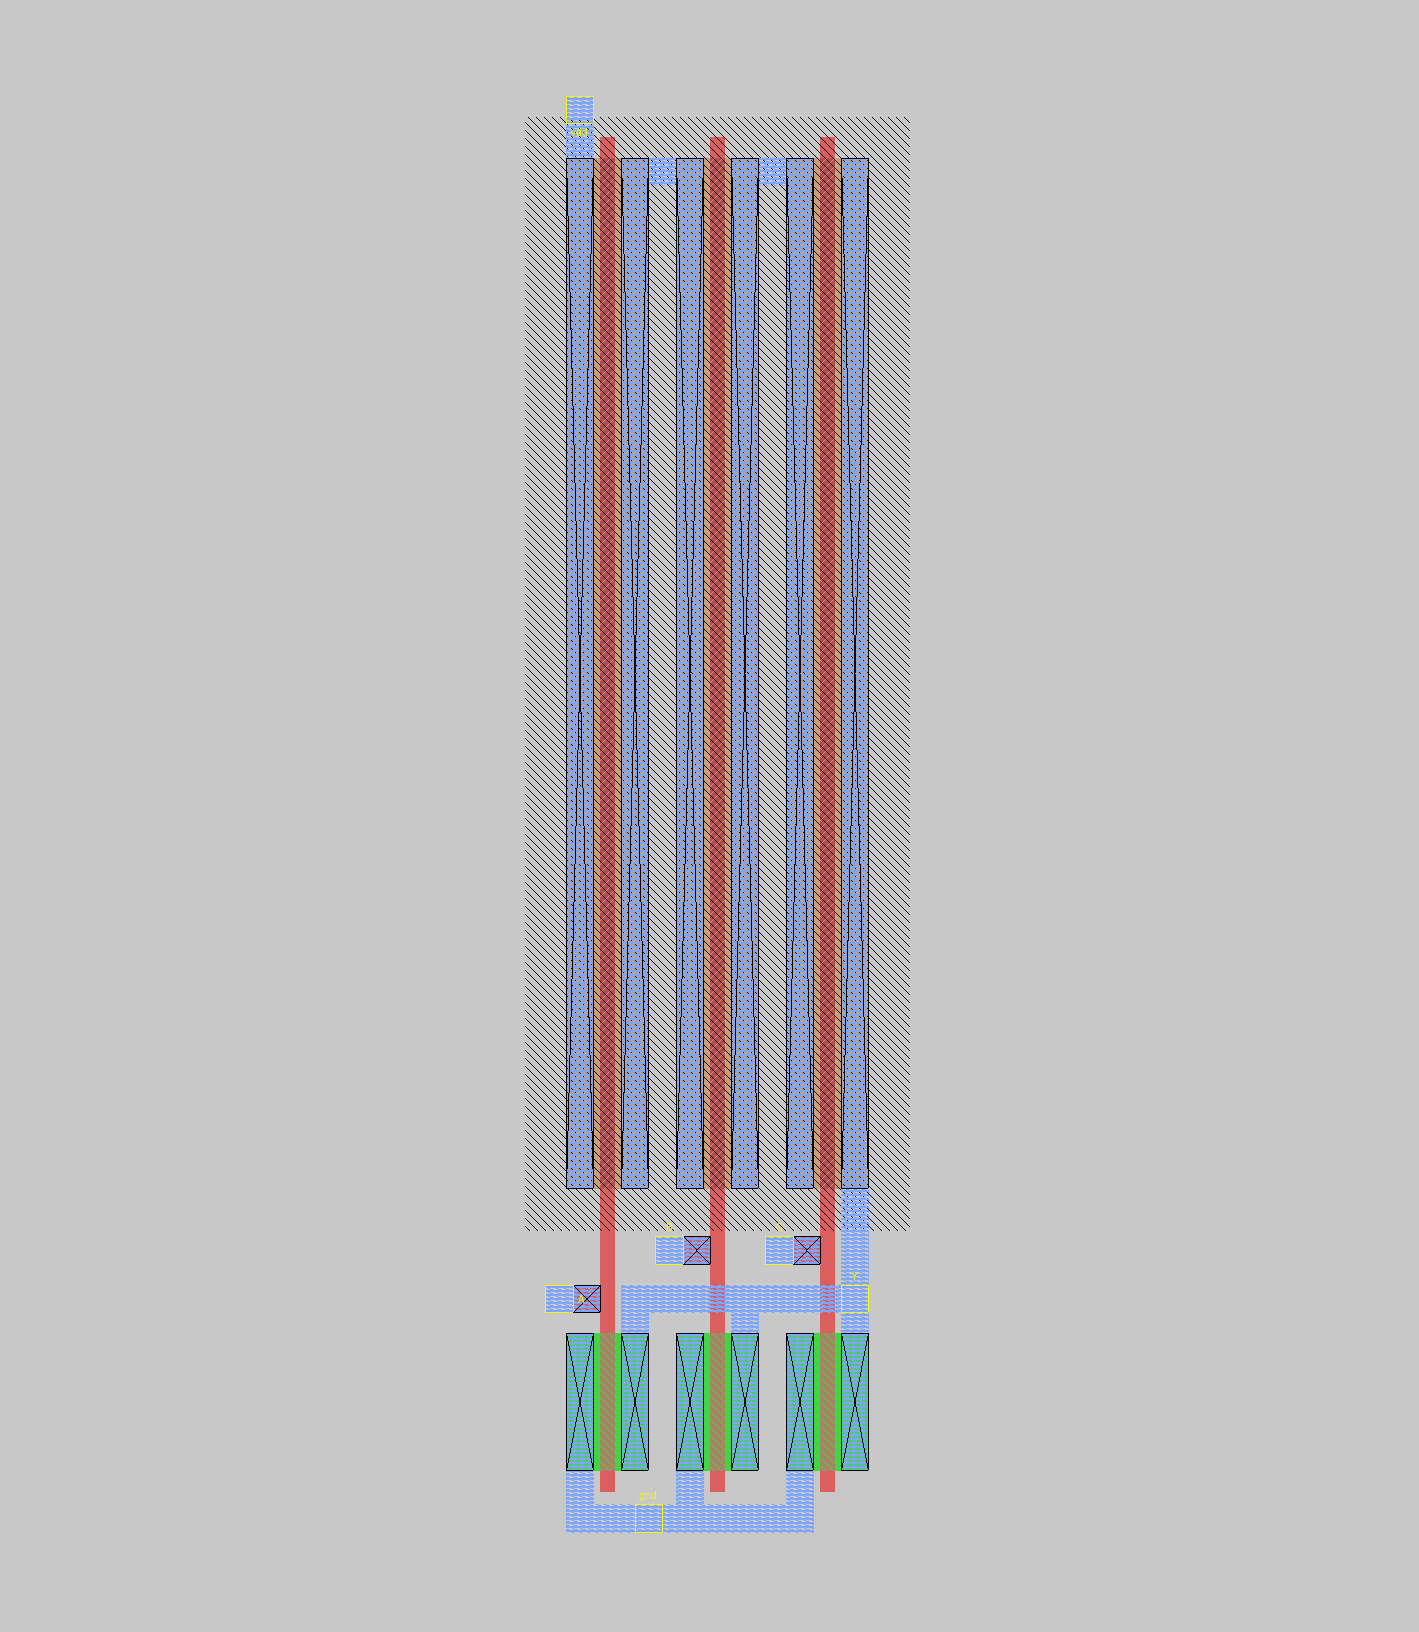
\includegraphics[width=\textwidth]{images/nor_3_cmos_layout.png}
            \caption{3 Input NOR}
        \end{subfigure} \\
        \begin{subfigure}{0.44\linewidth}
            \centering
            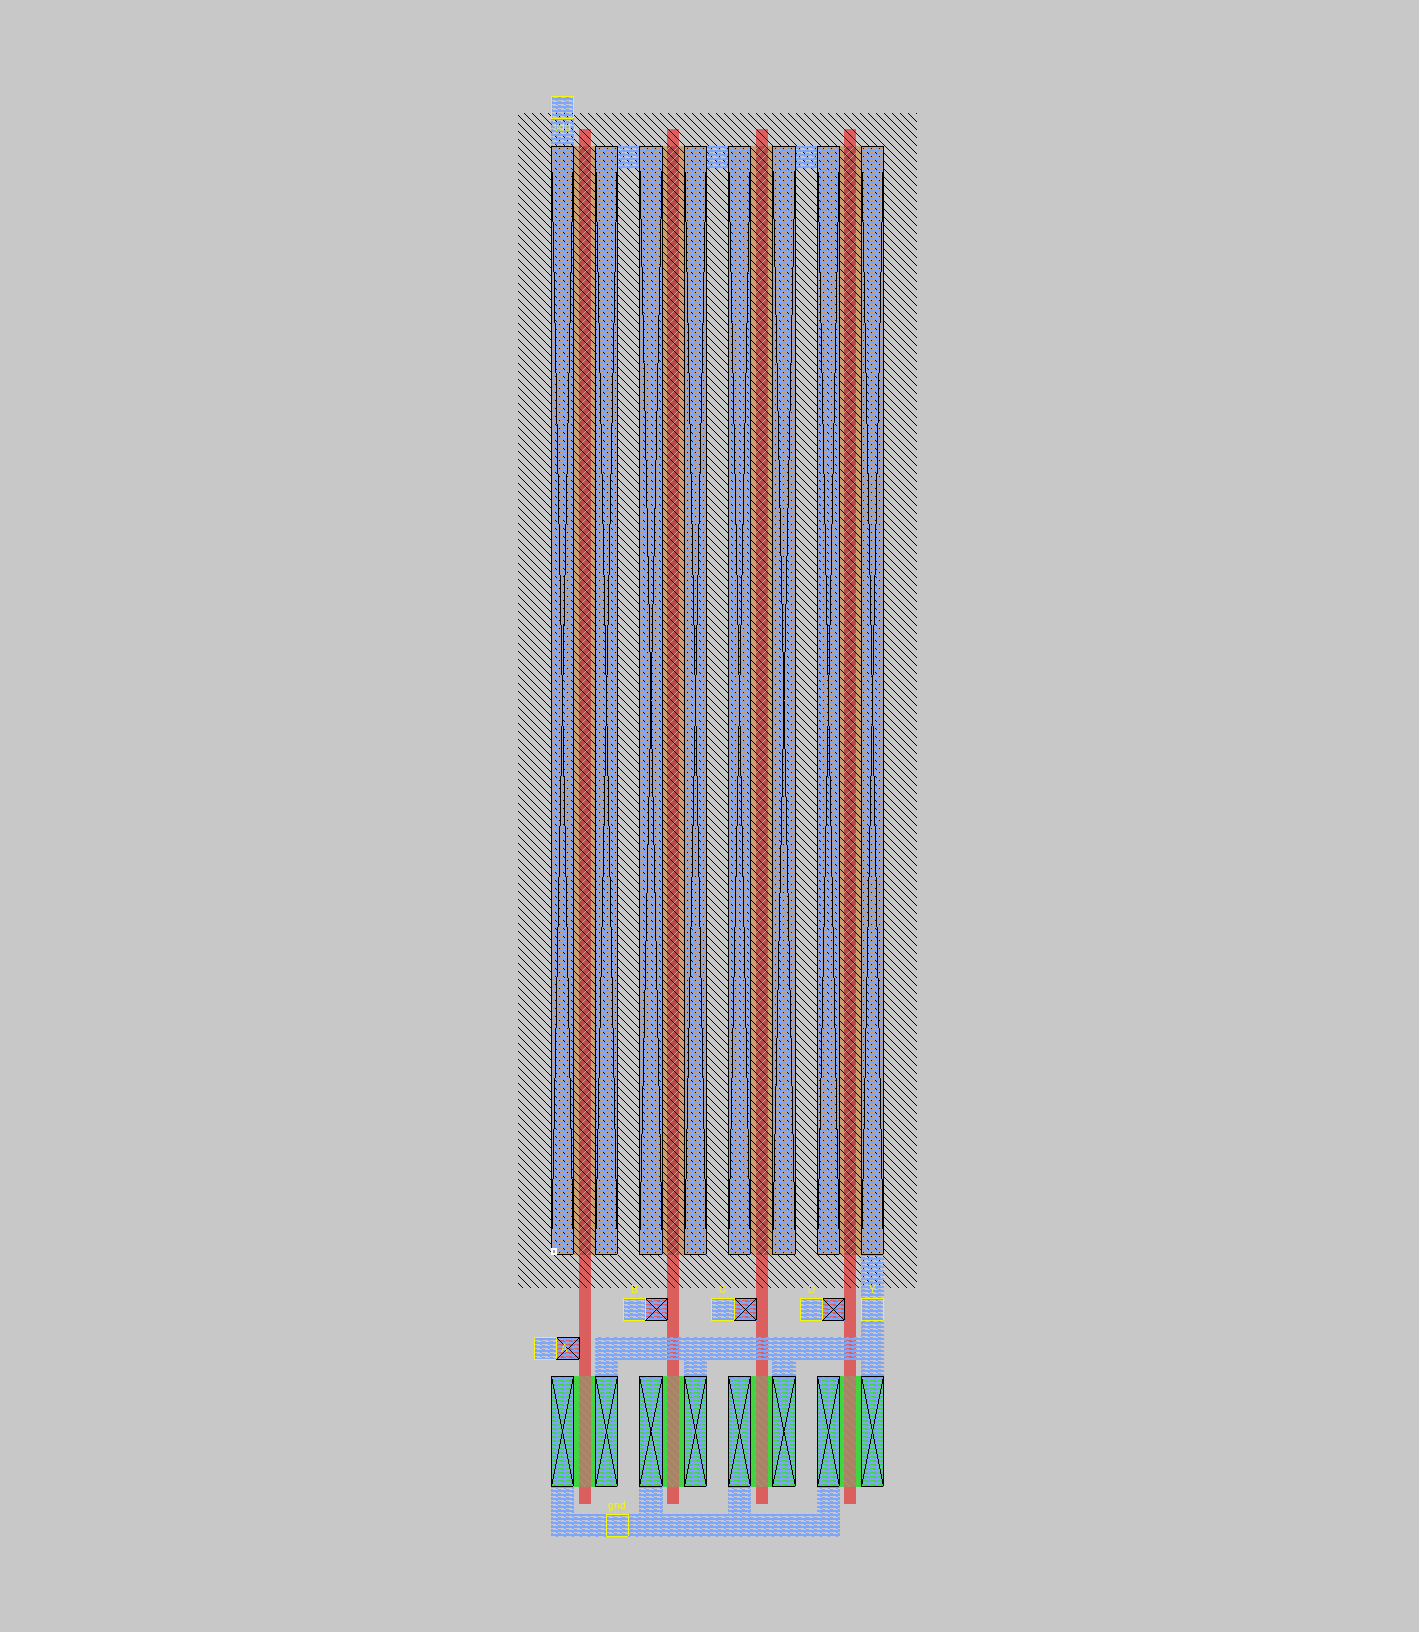
\includegraphics[width=\textwidth]{images/nor_4_cmos_layout.png}
            \caption{4 Input NOR}
        \end{subfigure} &
        \begin{subfigure}{0.44\linewidth}
            \centering
            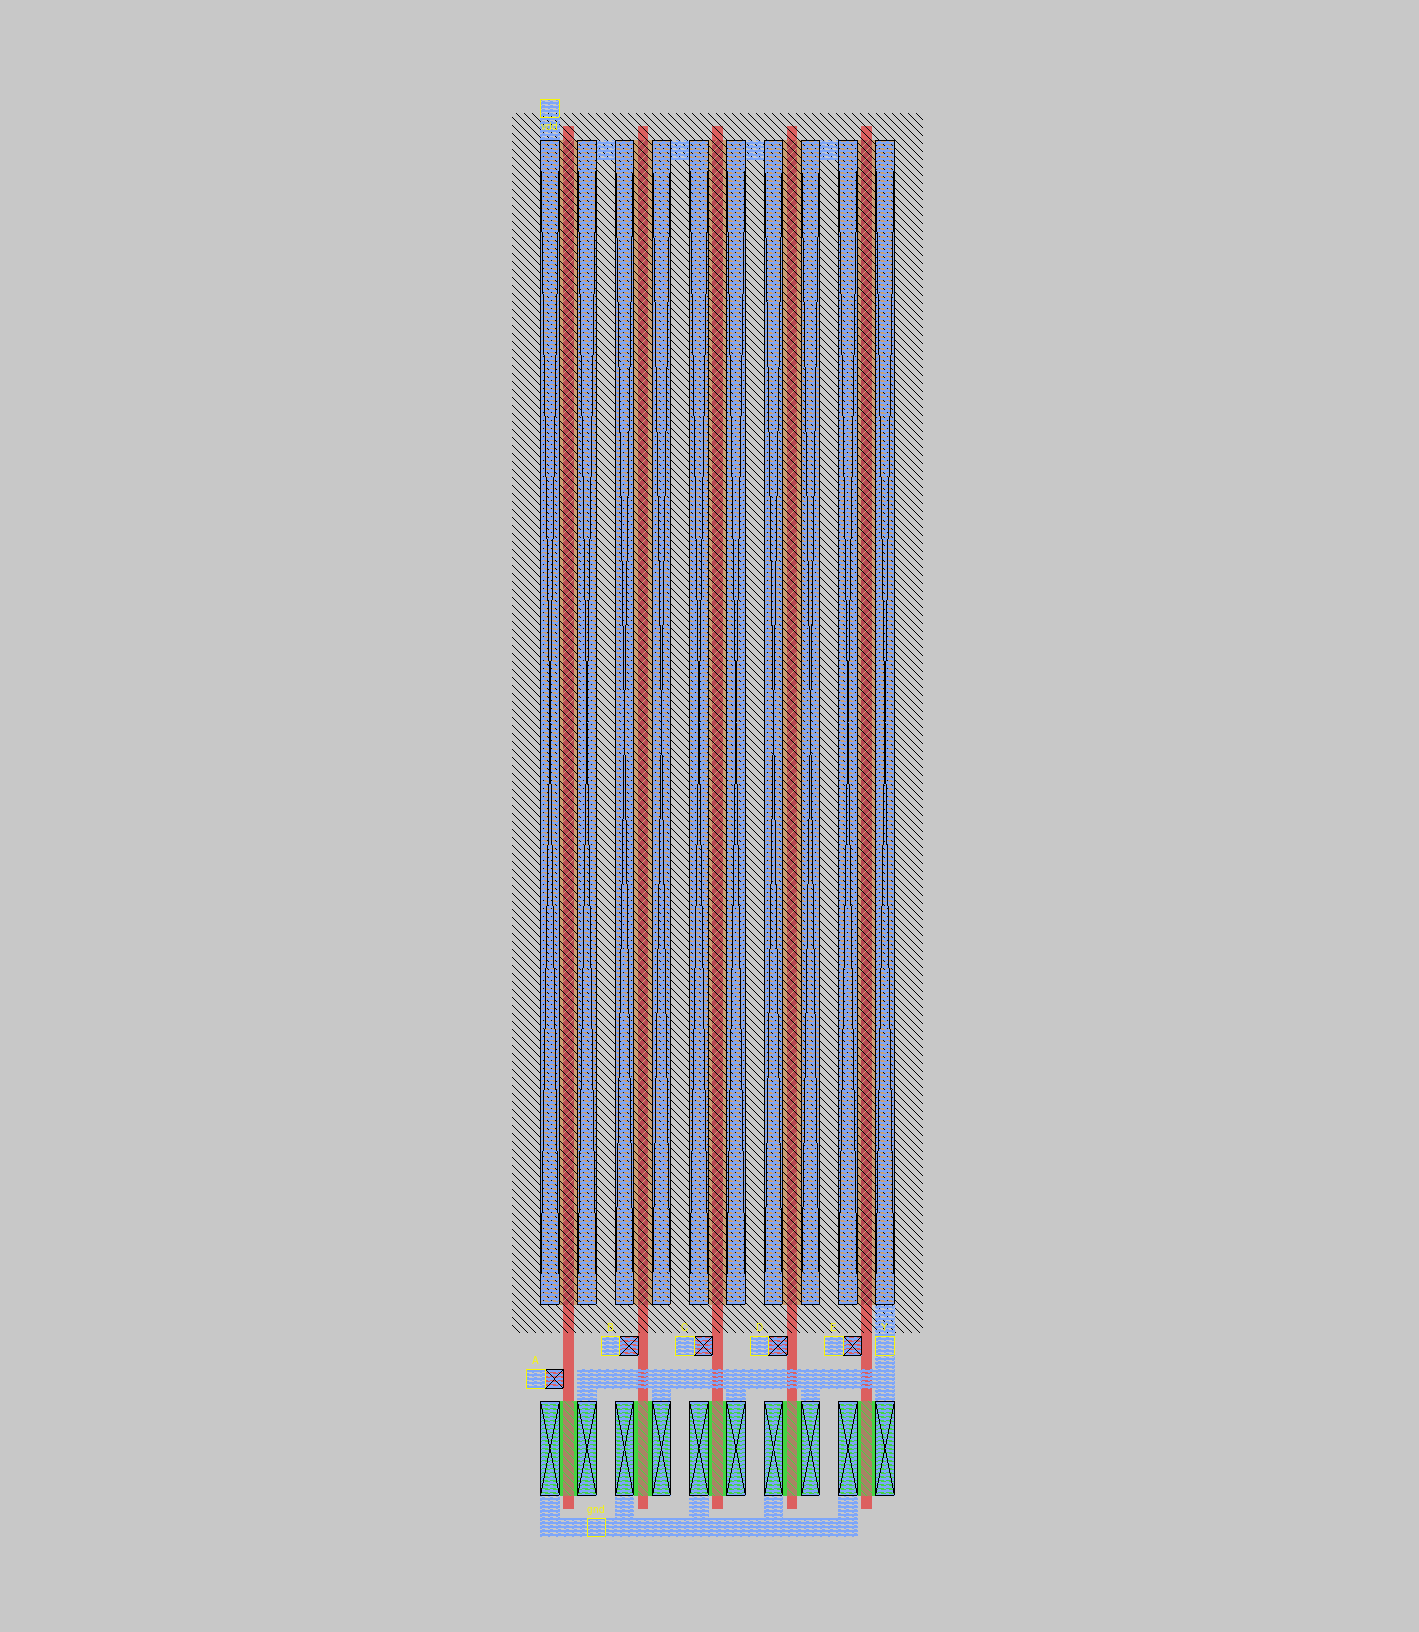
\includegraphics[width=\textwidth]{images/nor_5_cmos_layout.png}
            \caption{5 Input NOR}
        \end{subfigure}
    \end{tabular}
    \caption{MAGIC Layout of NOR Gates}
\end{figure}

\subsection{XOR Gate}

\begin{figure}[H]
    \centering
    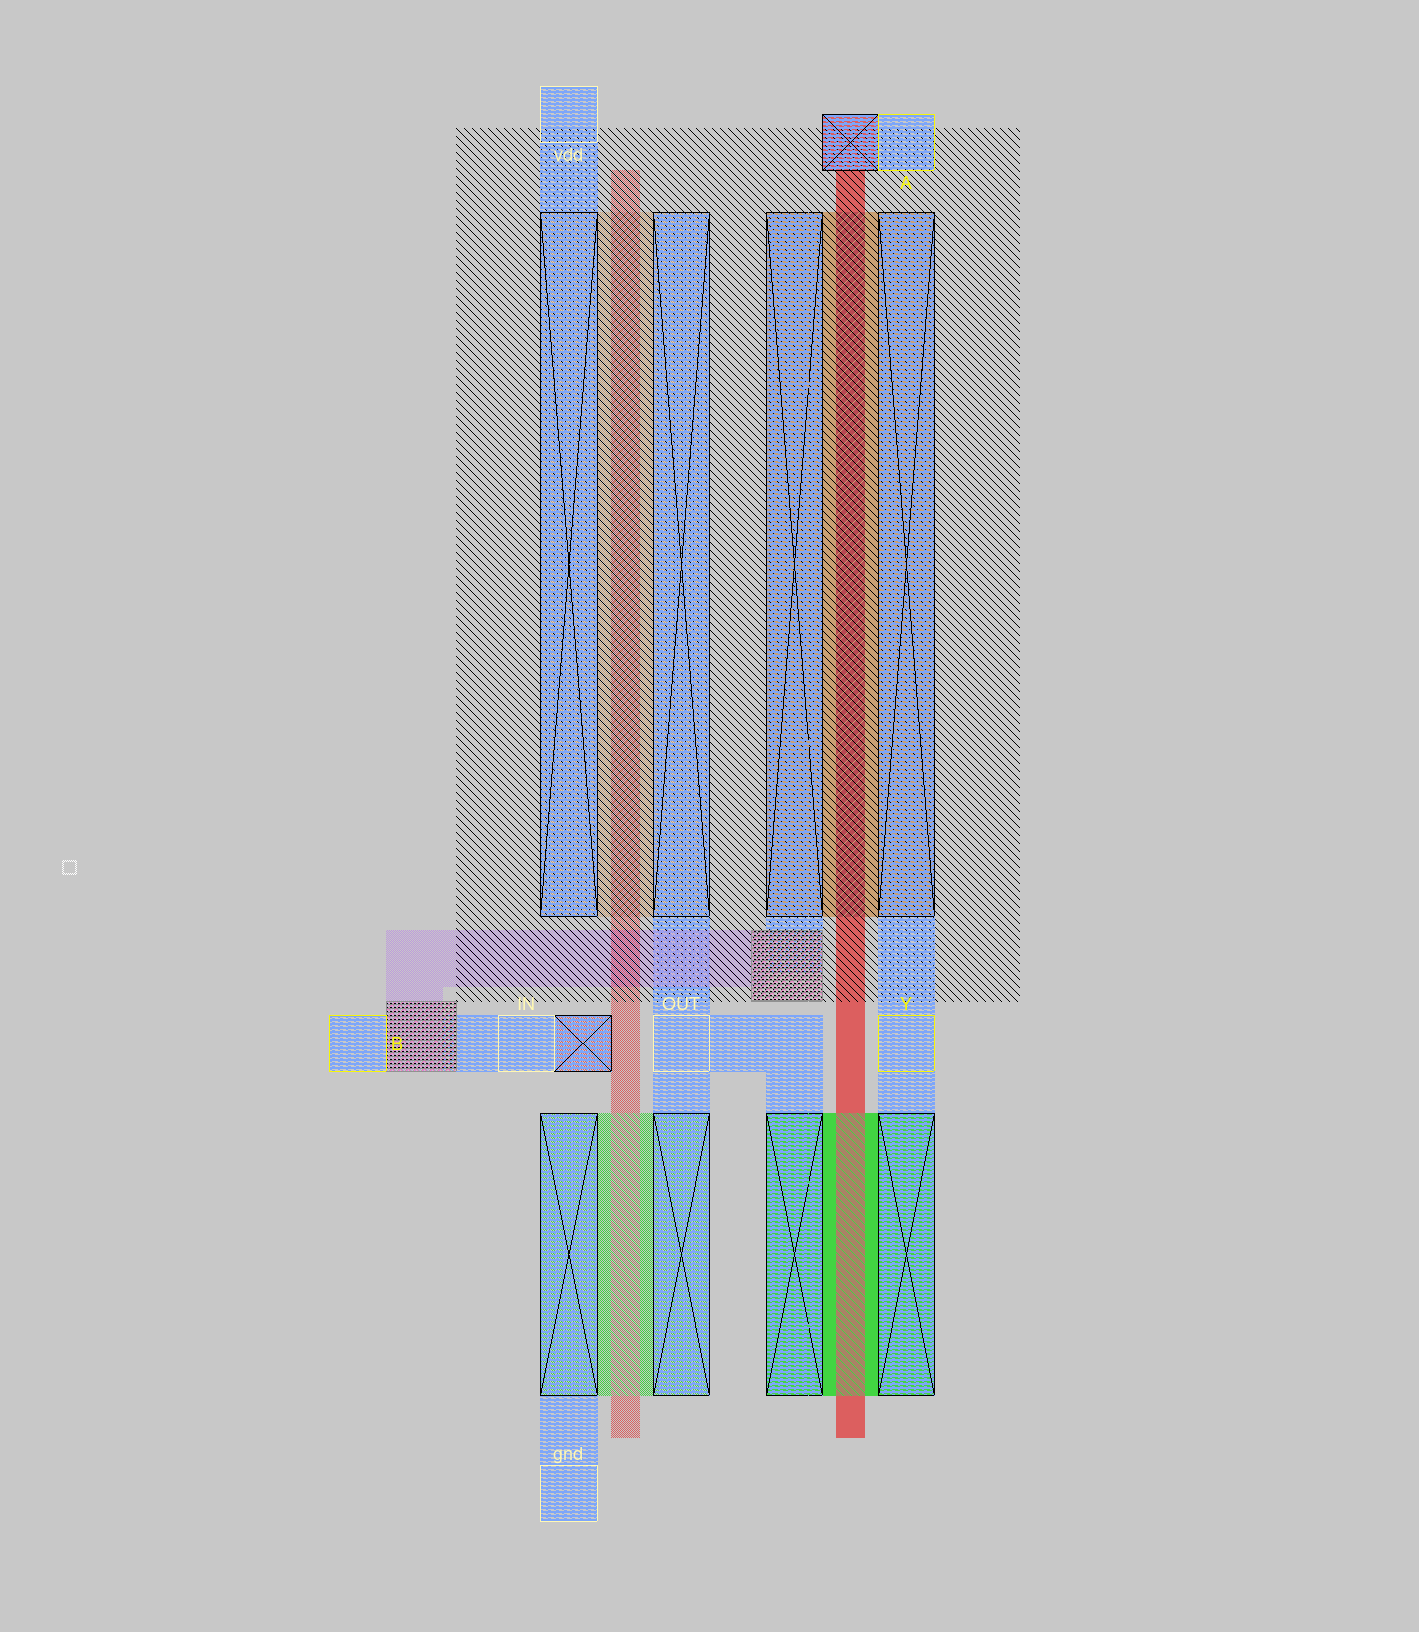
\includegraphics[width=0.48\textwidth]{images/xor_optimized_layout.png}
    \caption{MAGIC Layout of XOR Gate}
\end{figure}

\subsection{Propagate/Generate Generator}

\begin{figure}[H]
    \centering
    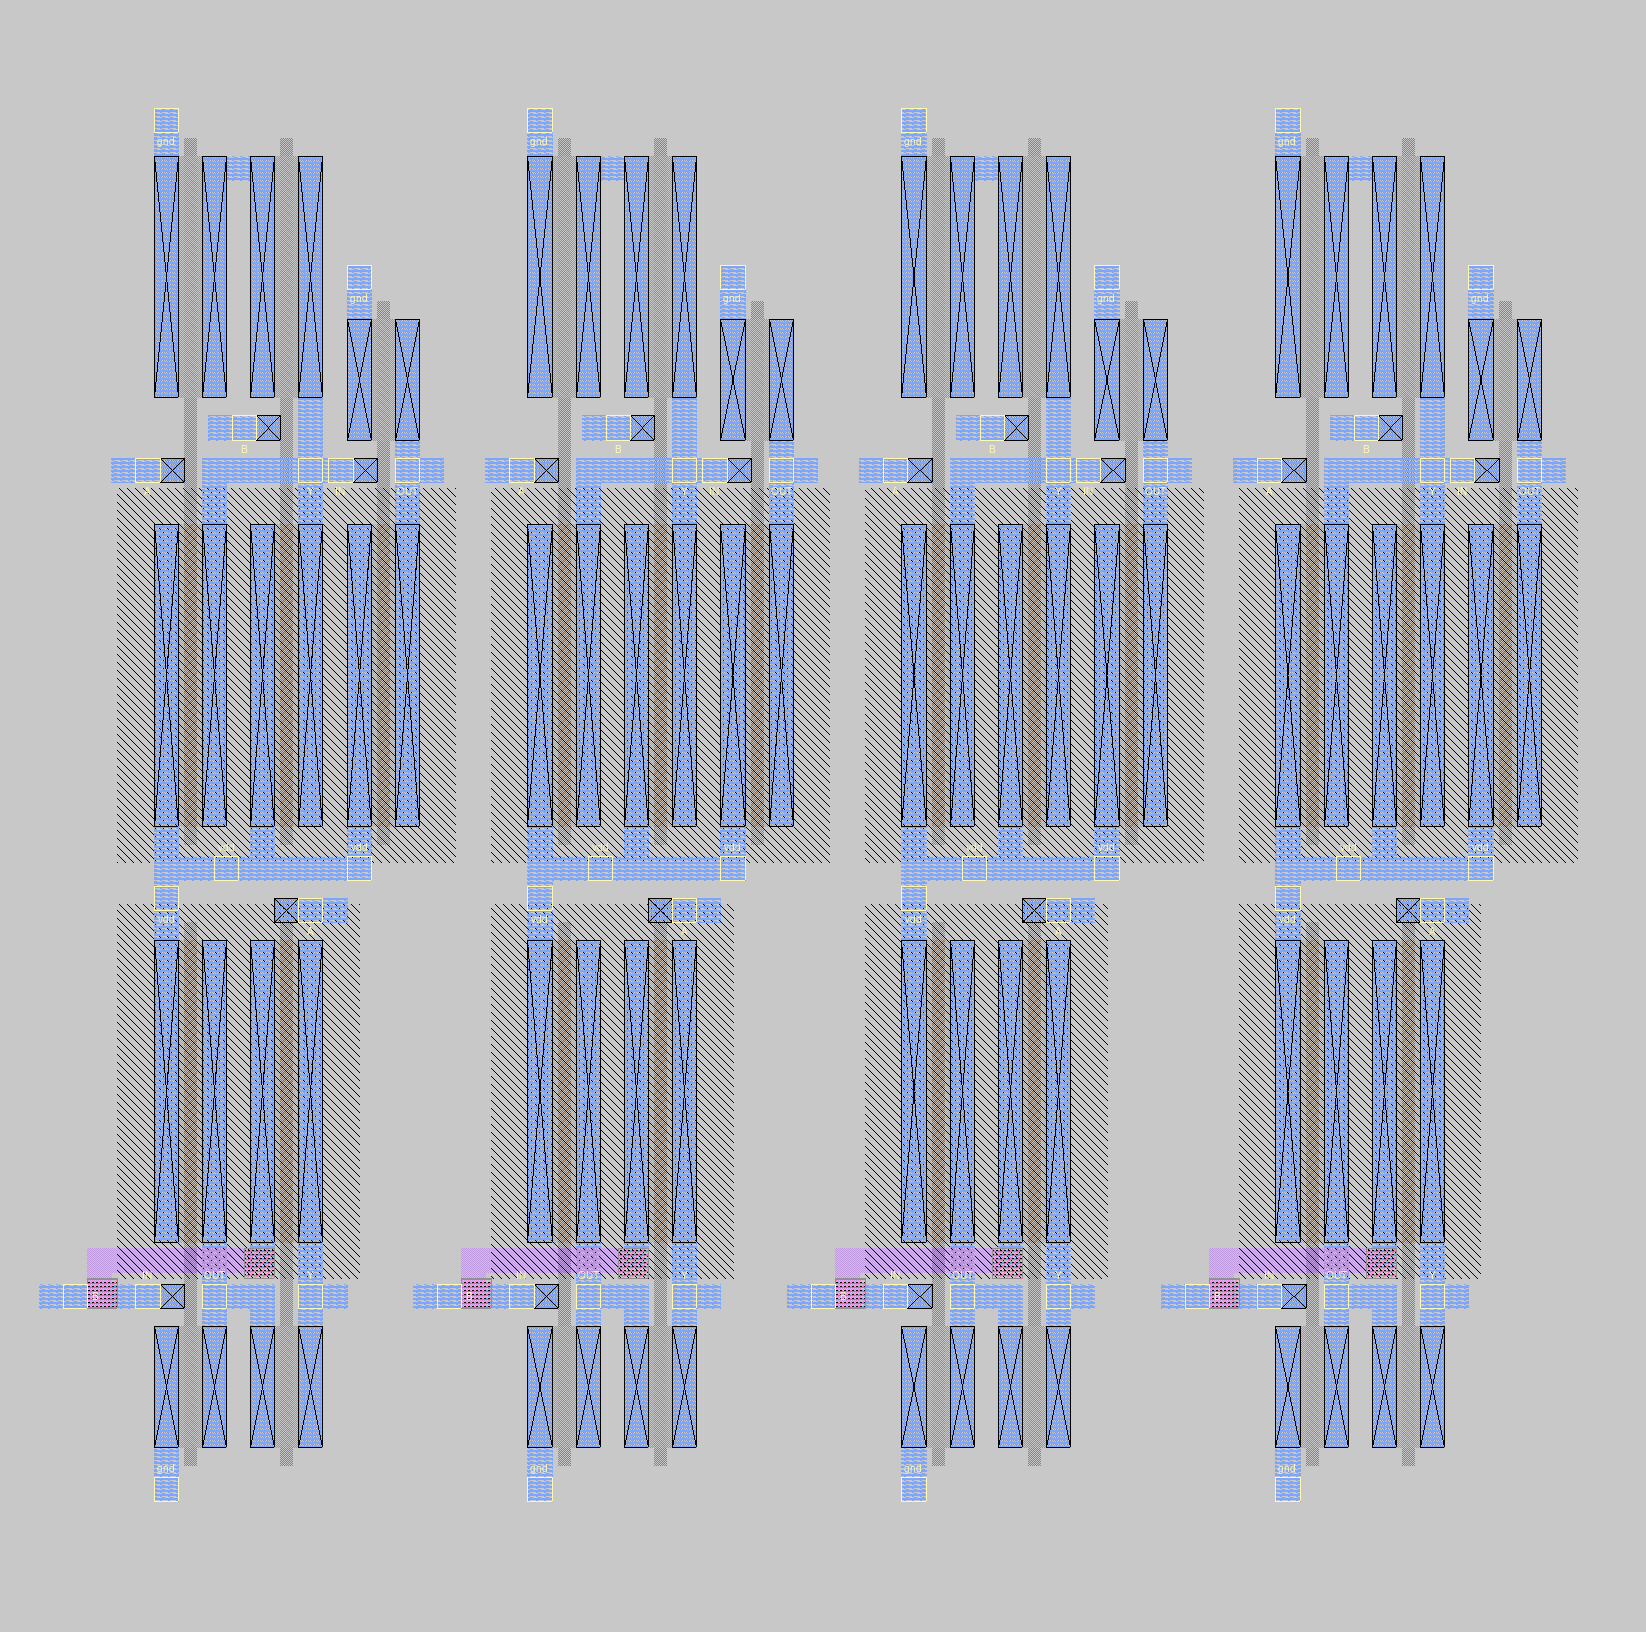
\includegraphics[width=0.48\textwidth]{images/pg_gen_optimized_layout.png}
    \caption{MAGIC Layout of Propagate/Generate Generator}
\end{figure}

\subsection{Carry Look Ahead Generator}

\begin{figure}[H]
    \centering
    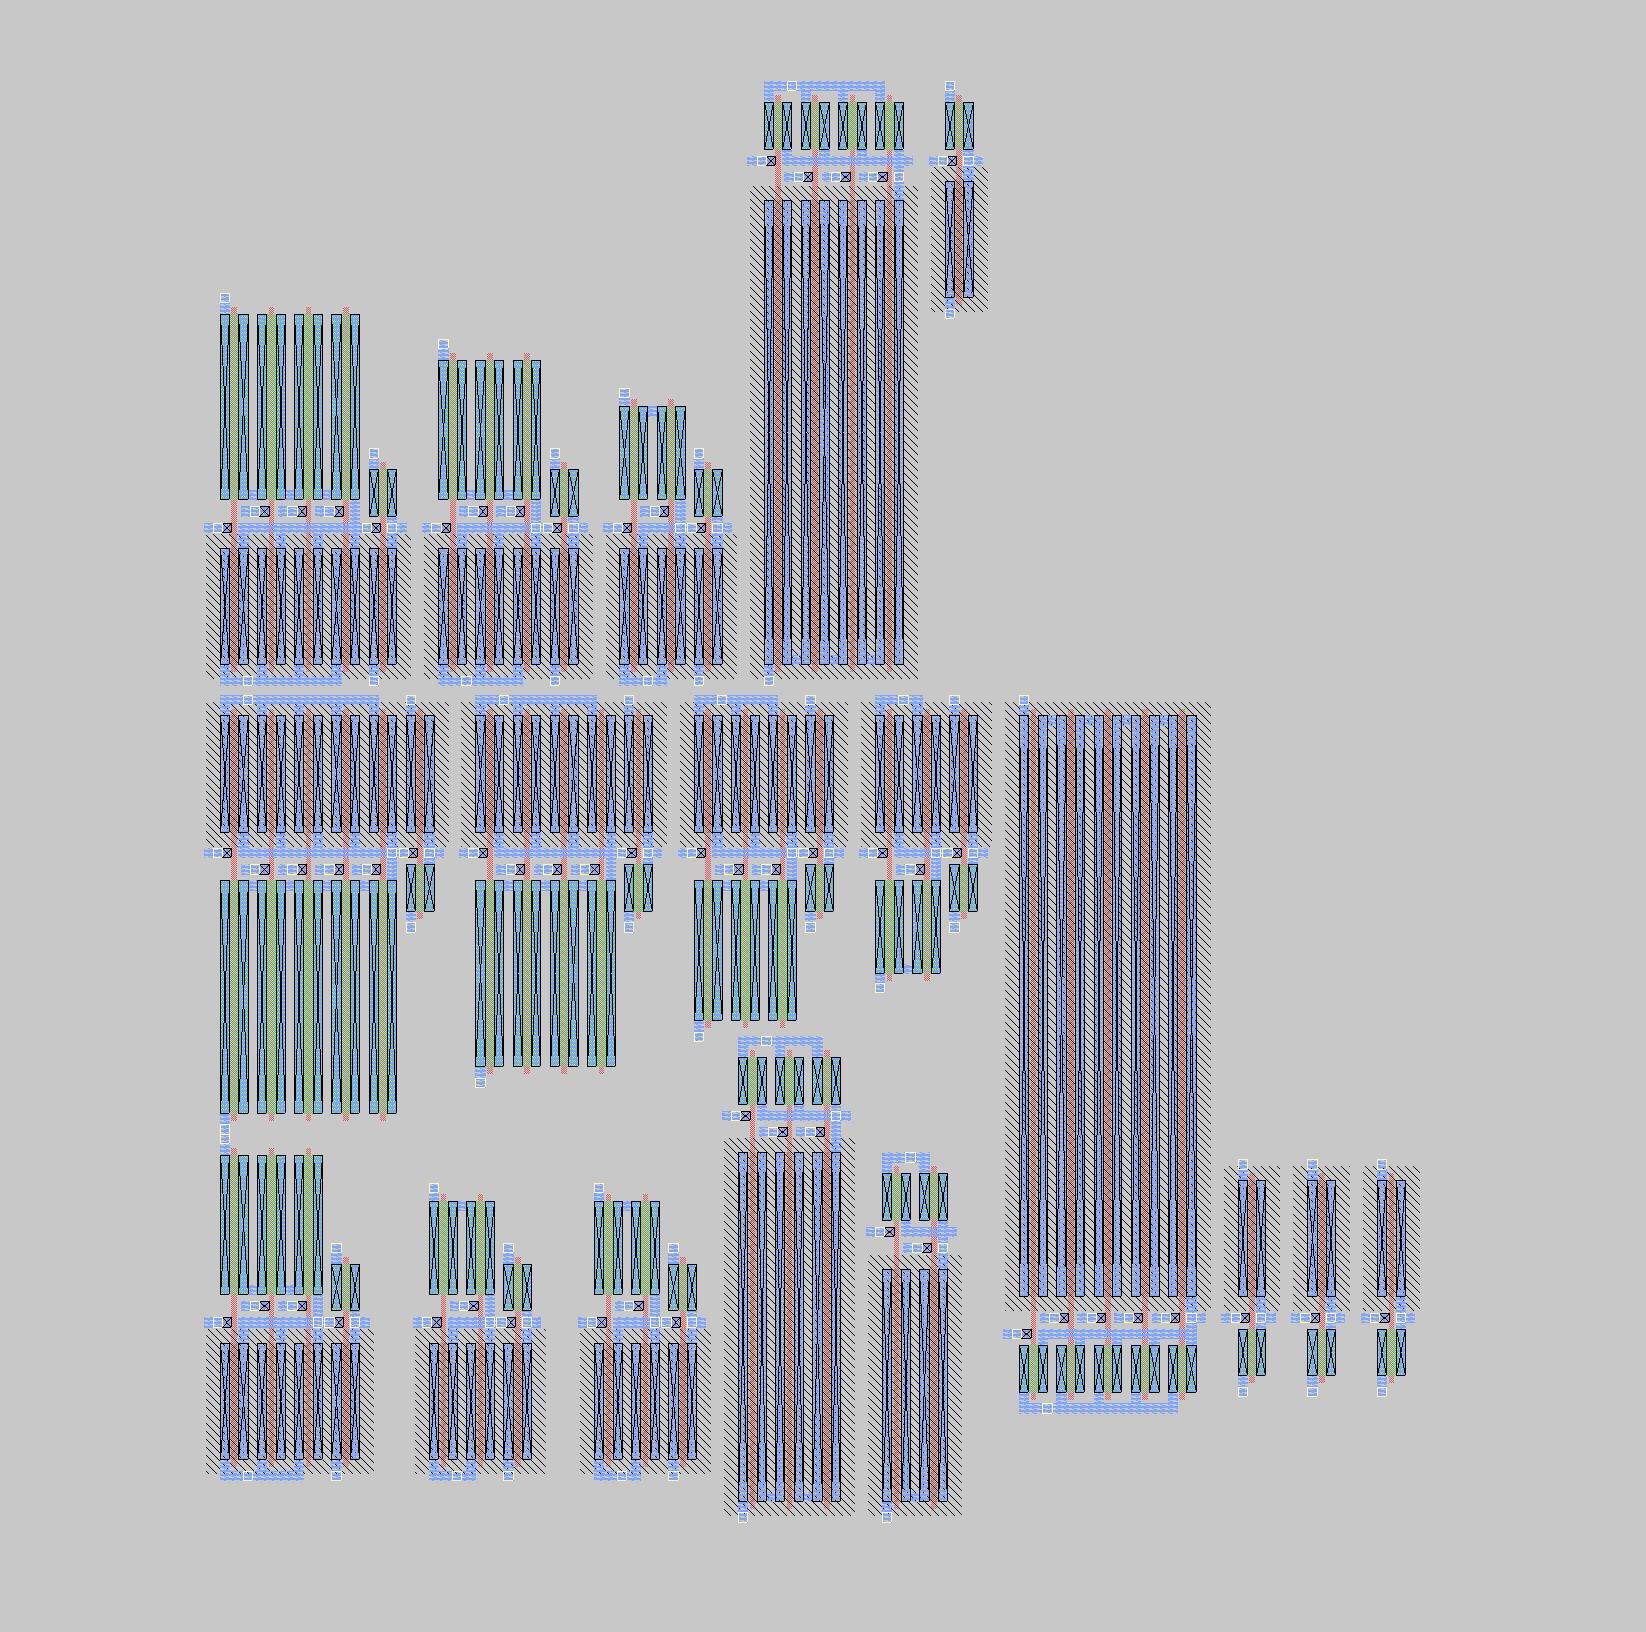
\includegraphics[width=0.48\textwidth]{images/cla_gen_cmos_layout.png}
    \caption{MAGIC Layout of Carry Look Ahead Generator}
\end{figure}

\subsection{Sum Generator}

\begin{figure}[H]
    \centering
    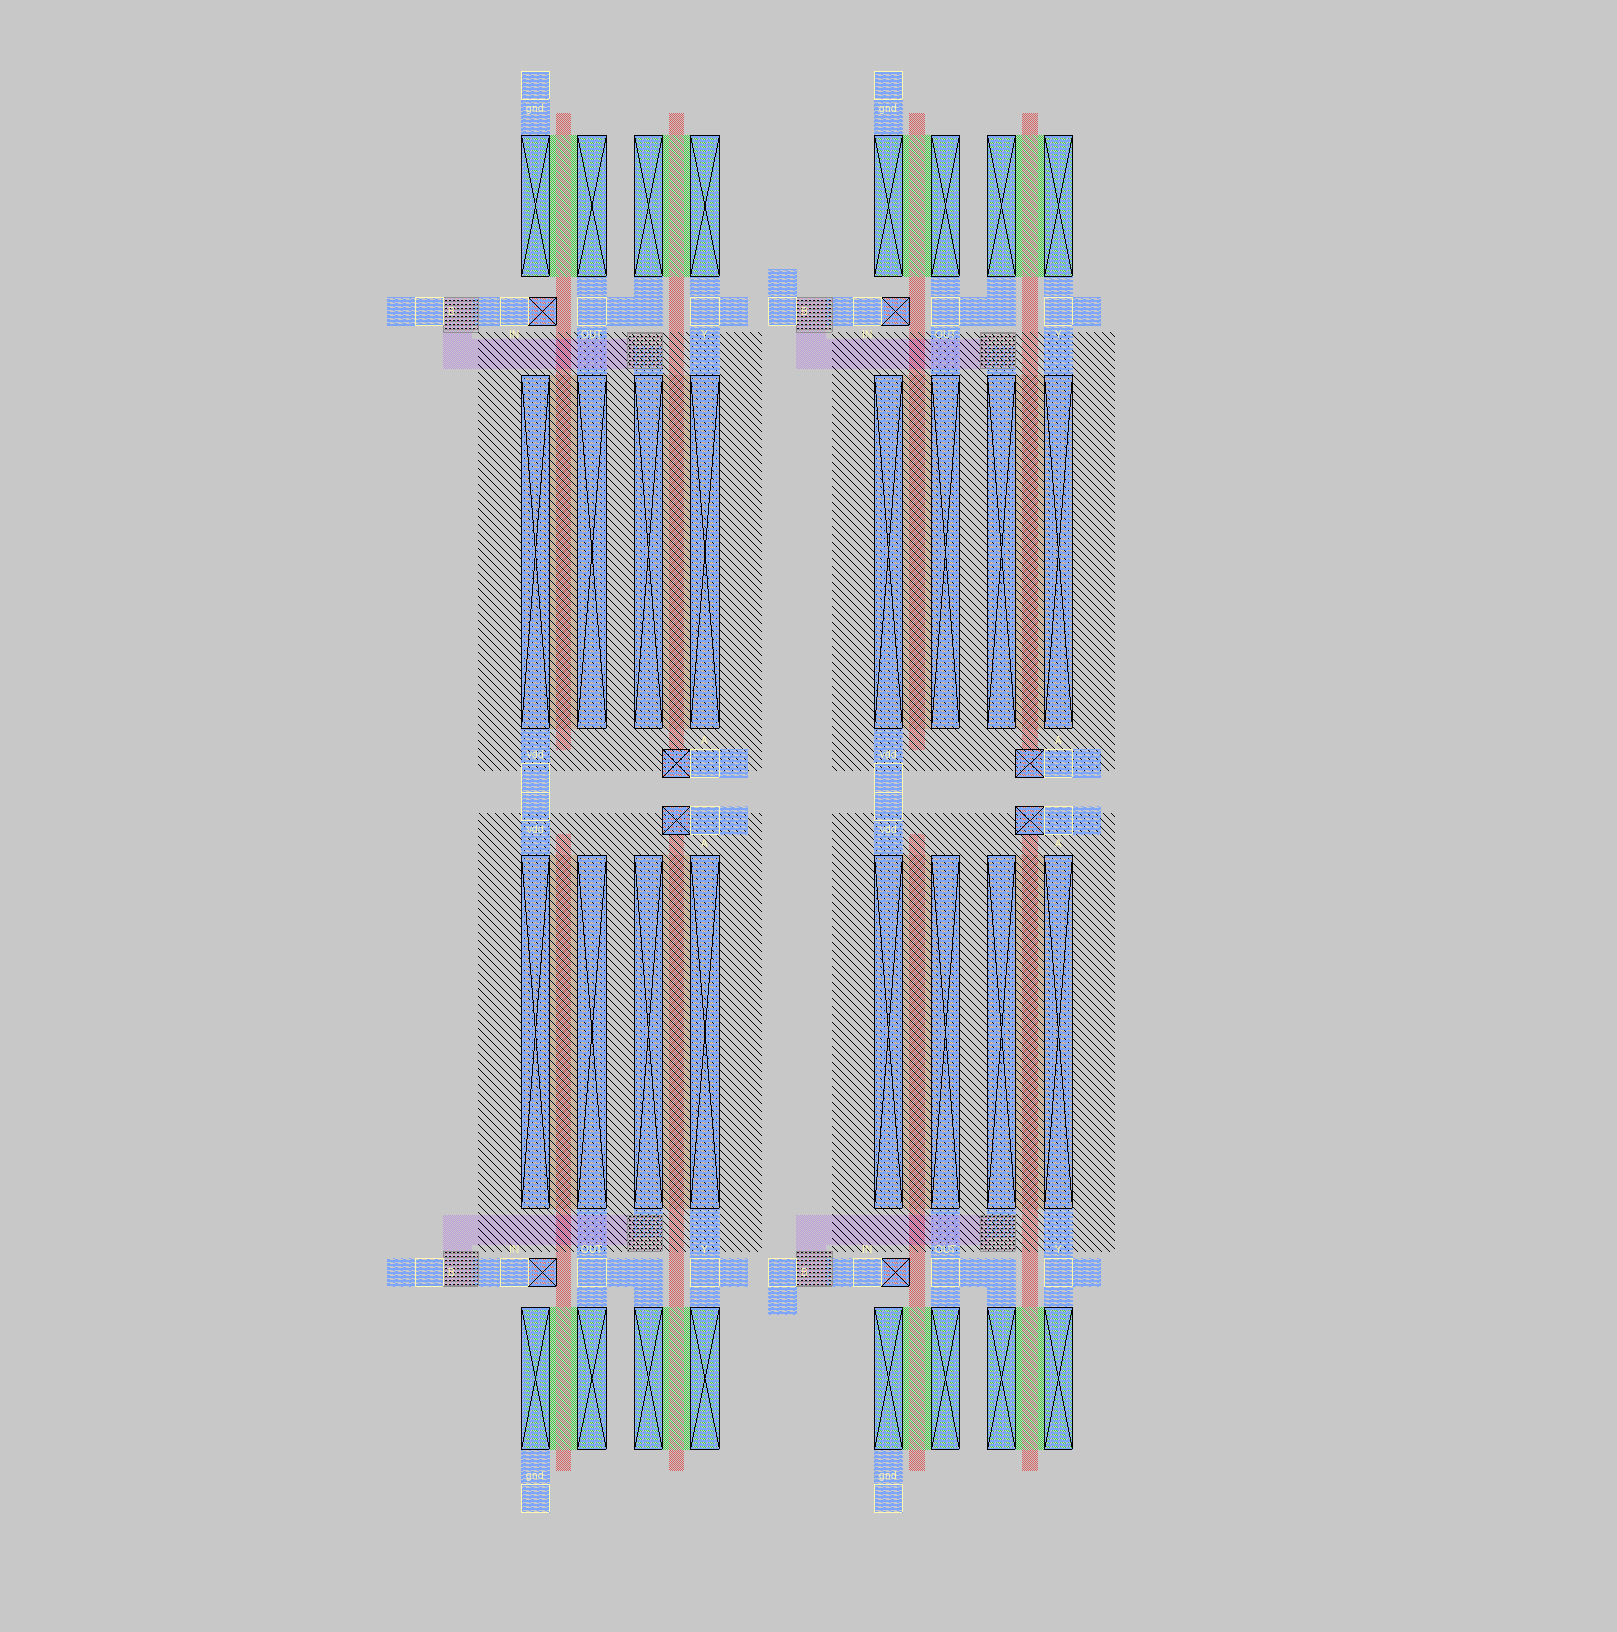
\includegraphics[width=0.48\textwidth]{images/sum_gen_optimized_layout.png}
    \caption{MAGIC Layout of Sum Generator}
\end{figure}

\subsection{D Flop Flop}

\subsubsection{CMOS Implementation}

\begin{figure}[H]
    \centering
    \includegraphics[width=0.48\textwidth]{images/d_ff_cmos_layout.png}
    \caption{MAGIC Layout of CMOS D Flip Flop}
\end{figure}

\subsubsection{Optimized Implementation}

\begin{figure}[H]
    \centering
    \includegraphics[width=0.48\textwidth]{images/d_ff_optimized_layout.png}
    \caption{MAGIC Layout of Optimized D Flip Flop}
\end{figure}


\subsection{Full Circuit}

\begin{figure*}[t]
    \centering
    \includegraphics[width=1\textwidth]{images/full_optimized_layout.png}
    \caption{MAGIC Layout of Full Circuit}
\end{figure*}

\section{Post Layout Simulation}

\subsection{Inverter}

\begin{figure}[H]
    \centering
    \includegraphics[width=0.48\textwidth]{images/inv_cmos_post_tran.eps}
    \caption{Post Layout NGSPICE Plot of Inverter}
\end{figure}

\subsection{NAND Gate}

\begin{figure}[H]
    \centering
    \begin{tabular}{cc}
        \begin{subfigure}{0.44\linewidth}
            \centering
            \includegraphics[width=\textwidth]{images/nand_cmos_post_tran.eps}
            \caption{2 Input NAND}
        \end{subfigure} &
        \begin{subfigure}{0.44\linewidth}
            \centering
            \includegraphics[width=\textwidth]{images/nand_3_cmos_post_tran.eps}
            \caption{3 Input NAND}
        \end{subfigure} \\
        \begin{subfigure}{0.44\linewidth}
            \centering
            \includegraphics[width=\textwidth]{images/nand_4_cmos_post_tran.eps}
            \caption{4 Input NAND}
        \end{subfigure} &
        \begin{subfigure}{0.44\linewidth}
            \centering
            \includegraphics[width=\textwidth]{images/nand_5_cmos_post_tran.eps}
            \caption{5 Input NAND}
        \end{subfigure}
    \end{tabular}
    \caption{Post Layout NGSPICE Plot of NAND Gates}
\end{figure}

\subsection{NOR Gate}

\begin{figure}[H]
    \centering
    \begin{tabular}{cc}
        \begin{subfigure}{0.44\linewidth}
            \centering
            \includegraphics[width=\textwidth]{images/nor_cmos_post_tran.eps}
            \caption{2 Input NOR}
        \end{subfigure} &
        \begin{subfigure}{0.44\linewidth}
            \centering
            \includegraphics[width=\textwidth]{images/nor_3_cmos_post_tran.eps}
            \caption{3 Input NOR}
        \end{subfigure} \\
        \begin{subfigure}{0.44\linewidth}
            \centering
            \includegraphics[width=\textwidth]{images/nor_4_cmos_post_tran.eps}
            \caption{4 Input NOR}
        \end{subfigure} &
        \begin{subfigure}{0.44\linewidth}
            \centering
            \includegraphics[width=\textwidth]{images/nor_5_cmos_post_tran.eps}
            \caption{5 Input NOR}
        \end{subfigure}
    \end{tabular}
    \caption{Post Layout NGSPICE Plot of NOR Gates}
\end{figure}

\subsection{XOR Gate}

\begin{figure}[H]
    \centering
    \includegraphics[width=0.48\textwidth]{images/xor_optimized_post_tran.eps}
    \caption{Post Layout NGSPICE Plot of XOR Gate}
\end{figure}

\subsection{D Flop Flop}

\begin{figure}[H]
    \centering
    \includegraphics[width=0.48\textwidth]{images/d_ff_optimized_post_tran.eps}
    \caption{Post Layout NGSPICE Plot of D Flip Flop}
\end{figure}

\begin{verbatim}
    t_cq                =  3.04861e-10ns
    t_su                =  4.72107e-10ns
    t_h                 =  2.88159e-10ns
\end{verbatim}

Post layout the D flip flop has a slower $t_{\text{cq}}$ but the setup and hold times are still at low ranges.

\subsection{Full Circuit (with Load Inverters)}

\begin{figure}[H]
    \centering
    \includegraphics[width=0.48\textwidth]{images/full_optimized_load_post_tran.eps}
    \caption{Post Layout NGSPICE Plot of Full Circuit}
\end{figure}

\section{FPGA Simulation}

\subsection{On Board LEDs}

\begin{figure}[H]
    \centering
    \begin{subfigure}{0.48\textwidth}
        \includegraphics[width=\linewidth]{images/fpga_1.png}
        \caption{1111 + 1111 + 0 = 11110}
    \end{subfigure}
    \hfill
    \begin{subfigure}{0.48\textwidth}
        \includegraphics[width=\linewidth]{images/fpga_2.png}
        \caption{1111 + 1111 + 1 = 11111}
    \end{subfigure}
    \hfill
    \begin{subfigure}{0.48\textwidth}
        \includegraphics[width=\linewidth]{images/fpga_3.png}
        \caption{1011 + 1001 + 1 = 10101}
    \end{subfigure}
    
    \caption{FPGA Simulation}
    \label{fig:main}
\end{figure}

\subsection{Waveform Visualization}

\begin{figure}[H]
    \centering
    \includegraphics[width=0.48\textwidth]{images/fpga_waveform.png}
    \caption{Viewing Waveform of FPGA Simulation}
\end{figure}

\section*{Acknowledgment}


\begin{thebibliography}{00}
    \bibitem{b1} Wikipedia, "Carry-lookahead adder." Available at: \url{https://en.wikipedia.org/wiki/Carry-lookahead_adder}.
    \bibitem{b2} Github, Repository with all project files Available at: \url{https://github.com/wig-nesh/vlsi-course-project}.
\end{thebibliography}
    
\end{document}


